\documentclass[letterpaper]{article} % DO NOT CHANGE THIS
\usepackage[submission]{aaai24}  % DO NOT CHANGE THIS
\usepackage{times}  % DO NOT CHANGE THIS
\usepackage{helvet}  % DO NOT CHANGE THIS
\usepackage{courier}  % DO NOT CHANGE THIS
\usepackage[hyphens]{url}  % DO NOT CHANGE THIS
\usepackage{graphicx} % DO NOT CHANGE THIS
\urlstyle{rm} % DO NOT CHANGE THIS
\def\UrlFont{\rm}  % DO NOT CHANGE THIS
\usepackage{natbib}  % DO NOT CHANGE THIS AND DO NOT ADD ANY OPTIONS TO IT
\usepackage{caption} % DO NOT CHANGE THIS AND DO NOT ADD ANY OPTIONS TO IT
\frenchspacing  % DO NOT CHANGE THIS
\setlength{\pdfpagewidth}{8.5in} % DO NOT CHANGE THIS
\setlength{\pdfpageheight}{11in} % DO NOT CHANGE THIS
\usepackage{graphicx}
\usepackage{latexsym}



% These are are recommended to typeset listings but not required. See the subsubsection on listing. Remove this block if you don't have listings in your paper.
\usepackage{newfloat}
\usepackage{listings}
\DeclareCaptionStyle{ruled}{labelfont=normalfont,labelsep=colon,strut=off} % DO NOT CHANGE THIS
\lstset{%
	basicstyle={\footnotesize\ttfamily},% footnotesize acceptable for monospace
	numbers=left,numberstyle=\footnotesize,xleftmargin=2em,% show line numbers, remove this entire line if you don't want the numbers.
	aboveskip=0pt,belowskip=0pt,%
	showstringspaces=false,tabsize=2,breaklines=true}


%
% Keep the \pdfinfo as shown here. There's no need
% for you to add the /Title and /Author tags.
\pdfinfo{
/TemplateVersion (2024.1)
}

%%%%%%%%%%%%%%
%%% ADDED FOR PAPER

\usepackage{algorithm}
\usepackage{algorithmic}


\usepackage{amsfonts,amsmath,amssymb} 
\usepackage{xcolor}
\usepackage{microtype}


\usepackage{graphicx}
\usepackage{subfigure}
\usepackage{multirow}
\usepackage{tabularx}

\setcounter{secnumdepth}{2} %May be changed to 1 or 2 if section numbers are desired.



\usepackage{booktabs} 

\graphicspath{ {./Images/} }
\newcommand{\tuple}[1]{\ensuremath{\left \langle #1 \right \rangle }}
\newcommand{\inconflict}{\textit{InConflict}}

% \newcommand{\plan}[1]{{\textcolor{blue}{[Plan: #1]}}}
% \newcommand{\guy}[1]{{\textcolor{red}{[Guy: #1]}}}
% \newcommand{\inon}[1]{{\textcolor{orange}{[Inon: #1]}}}
% \newcommand{\roni}[1]{{\textcolor{purple}{[Roni: #1]}}}
\newcommand{\plan}[1]{{\textcolor{blue}{[Plan: #1]}}}
\newcommand{\guy}[1]{\textcolor{blue}{[Guy: #1]}}
\newcommand{\inon}[1]{ }
\newcommand{\roni}[1]{ }
%\newcommand{\itay}[1]{\textcolor{green}{[#1]}}
\newcommand{\itay}[1]{}
\newcommand{\shortcite}[1]{{\cite{#1}}}
\newtheorem{definition}{Definition}

\title{Centralized Stochastic Multi-Agent Pathfinding under Partial Observability}

\begin{document}

\maketitle

\title{Centralized Stochastic Multi-Agent Pathfinding under Partial Observability}
% SUBMISSION 1013
% \author[A]{\fnms{First}~\snm{Author}\orcid{....-....-....-....}\thanks{Corresponding Author. Email: somename@university.edu.}}
% \author[B]{\fnms{Second}~\snm{Author}\orcid{....-....-....-....}}
% \author[B]{\fnms{Third}~\snm{Author}\orcid{....-....-....-....}} % use of \orcid{} is optional


% \address[A]{Short Affiliation of First Author}
% \address[B]{Short Affiliation of Second Author and Third Author}

\begin{abstract}
% ECAI Instructions: The abstract should contain no more than 200 words.
Multi-Agent Path Finding (MAPF) is the problem of finding paths for multiple agents where each agent aims to reach a given goal location without conflicting with the other agents. 
% In important MAPF applications such as an autonomous warehouse, the agents correspond to physical robots that are controlled in a centralized manner. 
% Physical robots often behave in a stochastic manner, do not have perfect localization, and may perform energy-consuming sensing actions to improve their localization. 
% While MAPF applications are often Physical robots often behave in a stochastic manner, do not have perfect localization, and may perform energy-consuming sensing actions to improve their localization. 
In MAPF applications with physical robots, we can expect the agents to have stochastic behavior and imperfect localization. 
Planning for such centrally-controlled agents can be viewed as a special case of Partially Observable Markov Decision Process (POMDP), but off-the-shelf POMDP solvers cannot scale to plan for even a very small number of agents, due to the exponentially large size of the state and action spaces.  
Instead, we propose the Online Prioritized Planning (OPP) approach, where each agent computes and follows its individually-optimal policy until a potential conflict is detected. 
OPP resolves detected potential conflicts by replanning online for a subset of the agents so as to avoid positions that are potentially occupied by other agents. 
We describe how OPP can be implemented and propose two extensions that encourage the agents to leverage localization actions when needed. 
We evaluate OPP and its extensions empirically to highlight the pros and cons of our approach and show it can scale better than an offline baseline.
\end{abstract}


%The page limit for ECAI scientific papers is {\bf 7} pages, plus one ({\bf 1}) additional page for references only. 


\section{Introduction}

% MAPF and SMAPF-PO
In classical multi agent path finding (MAPF) agents navigate in an environment represented as a graph.  Each agent must move from its current position to a given goal position without conflicting with other agents \cite{stern2019mapf}.
Real-world MAPF applications include automated logistic centers~\cite{wurman2008coordinating,salzman2020research}, airport towing~\cite{morris2016planning}, autonomous vehicles, robotics~\cite{veloso2015cobots}, and digital entertainment~\cite{ma2017feasibility}. However, MAPF research has mainly focused on deterministic and fully observable domains, i.e., where the effects of each action are known and deterministic and agents can fully observe their environment. 
%However, MAPF research has mainly focused on deterministic and fully observable domains, i.e., where the effects of each action are known and deterministic~\cite{SHARON201540,m-star,stern2019mapf} and the agents can fully observe their environment~\cite{wagner2017path,melchior2007particle,gonzalez2005planning}. 
Both assumptions, deterministic effects and full observability, are often violated in real-world problems, especially when the agents are physical robots. 
%For example, the wheels of a robot attempting to move forward may slip, causing it to move sideways, and the sensors responsible for localizing the robots may be noisy and limited, causing the robot's controller to be uncertain over its current location. 
This work addresses MAPF problems where both types of uncertainty exist, which we refer to as \emph{Stochastic MAPF with Partial Observability} (SMAPF-PO). 
% \textbf{Classical MAPF solvers, which scale to thousands of agents, cannot solve SMAPF-PO problems without compromising agents' safety.}  
Classical MAPF solvers cannot solve SMAPF-PO problems without compromising agents' safety. 

%\textbf{The first contribution of this work} is to formally define this type of MAPF problems, which we refer to as \emph{Stochastic MAPF with Partial Observability} (SMAPF-PO). 


% Often, one can define a probability distribution over the possible outcomes of an action, defining a Stochastic Multi-Agent Path Finding (SMAPF) problem that can be modeled as a Markov decision process (MDP) \cite{levy2022anOnline}. However, many real-world problems require partial observability. For example, the sensors of a robot cannot perceive the entire environment, or they cannot extract the needed data about the current state. 
% \plan{Define the problem as centralized POMDP, but it doesn't scale}\inon{DONE}


% Offline reduction
% We focus on solving SMAPF-PO problems in a centralized control setup. That is, a central planning agent receives at each step the observations of all agents, and dictates for each agent which action to take. 
% Centralized control is natural for SMAPF-PO problems that occur in an automated warehouse setting, where the robots are controlled by a  centralized warehouse management system. 
% \textbf{The second contribution of this work} is to show how, under the centralized control setup, a SMAPF-PO problem can be reduced to a single-agent Partially Observable Markov Decision Process (POMDP) over states and actions that represent the agents' joint positions and actions. 
% % OPP
% As expected, solving this exponentially large single-agent POMDP is only practical for very small problems. 
% To this end, we propose the \emph{Online Prioritized Planning (OPP)} approach for solving SMAPF-PO problem, which 
% is \textbf{the third contribution of this work}. 
% %OPP is based on \emph{Prioritized Planning} (PP)~\cite{silver2005cooperative}, which is arguably the most common approach to solve practical classical MAPF problems~\cite{}. 
% OPP is inspired by \emph{Prioritized Planning} (PP)~\cite{silver2005cooperative}, arguably the most common approach to solve practical classical MAPF problems, yet implementing PP for SMAPF-PO is not trivial. 
% OPP starts by computing offline a single-agent policy for each agent independently, ignoring all other agents. 
% The agents execute these policies until according to the current belief over the agents' current location indicate that a conflict may occur in the nearby future if the agents continue to execute their current policies. 
% At this stage OPP attempts to resolve potential conflicts by replacing the individually-optimal policy of some agents with policies that avoid the conflict. This planning is done online, to avoid the need to plan a-priori for every contingency. Finally, OPP employs a dedicated mechanism to encourage agents to optimize their policy over time. 
% We discuss several design choices and challenges when implementing OPP, and propose two extensions designed to encourage the agents to intelligence perform localization action when needed.  


% Centralized control, i.e., where  a central controller receives at each step the observations of all agents and dictates for each agent which action to take, is natural for SMAPF-PO problems that occur in an automated warehouse setting, where the robots are controlled by a  centralized warehouse management system. 
We consider SMAPF-PO problems in which the agents are controlled in a centralized manner, e.g., a warehouse management system. 
Such SMAPF-PO problem can be reduced to a single-agent Partially Observable Markov Decision Process (POMDP) over states and actions that represent the agents' joint positions and actions. Solving this exponentially large POMDP is only practical for extremely small problems, even with modern online POMDP solvers. Even Dec-POMDP solvers, which are designed for solving multi-agent problems~\cite{amato2019modeling} can scale to solve problems with approximately 180K states, while SMAPF-PO with only 4 agents on a 20x10 grid reaches 1G states, 625 actions, and 2K observations. 
Thus, off-the-shelf POMDP and Dec-POMDP solvers only handle tiny SMAPF-PO problems. 


%, which  is \textbf{the third contribution of this work}. 
%OPP is based on \emph{Prioritized Planning} (PP)~\cite{silver2005cooperative}, which is arguably the most common approach to solve practical classical MAPF problems~\cite{}. 
%OPP is inspired by \emph{Prioritized Planning} (PP)~\cite{silver2005cooperative}, arguably themost common approach to solve practical classical MAPF problems, yet implementing PP for SMAPF-PO is not trivial. 

% Inspired by the \emph{Prioritized Planning} (PP)~\cite{silver2005cooperative} approach to solve classical MAPF problems, 
% Inspired by \emph{Prioritized Planning} (PP)~\cite{silver2005cooperative} for classical MAPF, 
% we propose the \emph{Online Prioritized Planning (OPP)} approach for solving SMAPF-PO problems. 
% OPP starts by computing offline a single-agent policy for each agent independently, ignoring all other agents. 
% The agents execute these policies until according to the current belief over the agents' current location indicate that a conflict may occur in the nearby future if the agents continue to execute their current policies. 
% At this stage OPP attempts to resolve potential conflicts by replacing the individually-optimal policy of some agents with policies that avoid the conflict. This planning is done online, to avoid the need to plan a-priori for every contingency. Finally, OPP employs a dedicated mechanism to encourage agents to optimize their policy over time. 
% We discuss several design choices and challenges when implementing OPP, and propose two extensions designed to encourage the agents to intelligently perform localization action when needed.  

Inspired by \emph{Prioritized Planning} (PP)~\cite{silver2005cooperative} for classical MAPF, 
we propose the \emph{Online Prioritized Planning (OPP)} approach for solving SMAPF-PO problems. 
OPP starts by computing a single-agent policy for each agent independently, ignoring all other agents. 
The agents execute these policies until the belief over the agents' current location indicates a conflict may occur. % in the nearby future if the agents continue to execute their current policies. 
At this stage, OPP attempts to resolve potential conflicts by replacing the individually-optimal policy of some agents with policies that avoid the conflict. This planning is done online, to avoid the need to plan a-priori for every contingency. Finally, OPP employs a dedicated mechanism to encourage agents to optimize their policy over time. 
We discuss several design choices and challenges when implementing OPP, and propose two extensions designed to encourage the agents to intelligently perform localization action when needed.  

% The main contribution in our paper, as in most of MAPF research, is in describing a decoupling method that allows us to avoid directly solving the joint problem, considering all agents together. Instead we show how the decoupled single-agent problems that we solve allow us to scale to problems many orders of magnitude larger than a standard POMDP solver can handle over the joint problem. A secondary contribution is a set of problem specific modifications for the underlying POMDP solver, that provide additional leverage in the navigation and localization task that we define.
Our main contribution is a decoupling method that allows us to avoid directly solving the joint problem. The proposed method, OPP, allow us to scale to problems many orders of magnitude larger than a standard POMDP solver can handle over the joint problem. A secondary contribution is a set of problem-specific modifications for the underlying POMDP solver, that provide additional leverage in the navigation and localization task that we define. 
Experimental results over 12 SMAPF-PO problems show that, as expected, POMDP solvers over the joint problem cannot scale beyond tiny grids with two agents in reasonable time. OPP with our extensions, however, can solve non-trivial problems with up to 4 agents.%\footnote{The benchmark problems we used in our experiments will be made publicly available to support future research.}



  

% Where classical MAPF solvers can scale to thousands of agents, 

% but they cannot solve SMAPF-PO problems without compromising agents' safety.  
% On the other hand, offline POMDP-based baselines can guarantee safety but cannot scale to non-trivial problems with more than 

% Results
% We also report on an experimental evaluation of several versions of OPP and a comparison to an off-the-shelf POMDP-based solver that attempts to find an optimal joint policy offline. 
% For this evaluation, we created a benchmark of 12 SMAPF-PO problems with different agent interactions. 
% Our results highlight that SMAPF-PO is an extremely hard problem. 
% On the one hand, classical MAPF solvers can scale to thousands of agents, but they cannot solve SMAPF-PO problems without compromising agents' safety.  
% On the other hand, offline POMDP-based baselines can guarantee safety but cannot scale to non-trivial problems with more than two agents. OPP with its extensions provides the first step towards solving non-trivial problems, finding solutions for up to 4 agents in our evaluation.\footnote{The benchmark problems we used in our experiments will be made publicly available to support future research.}  

%can solve larger problems. %, including a problem with 4 agents. 
% Our results highlight that SMAPF-PO is an extremely hard MAPF variant, %even under the centralized control setup, 
% suggesting SMAPF-PO as an open challenge for future research.



% In particular, we show that off-the-shelf POMDP solvers are ill-suited to be used in this context, and proposed an enhanced version of FSVI that works well. In addition, we introduce a  timer-based method to allow agents to optimize their behavior based on observations collected over time. 
% Another contribution is that we introduce a method to force localization when needed. [[bad writing of this 

% future work. %where solving problems with even a small number of agents is computationally intractable. This suggests % already computationally exhaustive
% \inon{later we'll add more scenarios to test our algorithm's sensitivity to different aspects of the model}

% The main contributions of this work are as follows. 
% First, we introduce the XXX problem. 
% Second, we propose an offline approach to solve the problem and show that it cannot scale. 
% Third, we propose online approach to solve the problem, where joint planning only occurs when conflicts are detected in the near future.  
% Fourth, we propose a method for performing this joint planning, based on the well-known prioritized planning method in MAPF,
% which relies on only solving single-agent POMDP solvers subject to some forms of constraints to avoid future conflicts. 
% Implementing prioritized planning in our setting is not trivial. 
% In particular, we show that off-the-shelf POMDP solvers are ill-suited to be used in this context, and proposed an enhanced version of FSVI that works well. In addition, we introduce a  timer-based method to allow agents to optimize their behavior based on observations collected over time. 
% Another contribution is that we introduce a method to force localization when needed. [[bad writing of this contribution]]



% solution
% We discuss several design choices and challenges when implementing OPP, and propose two extensions. 
% The first includes 


% agents' current beliefs over their possible whereabouts indicate they are within a predefined distance of each other, we use forward expansion to decide if they may collide in the next couple of steps if they follow their current policies. 
% %\plan{explain the replanning phase - forbidden states, timers, dominance ...}
% %\inon{DONE}
% If so, we replan for one of the agents involved in the potential collision, by forbidding it to reach the states that any other agent may visit until the moment of the possible collision. We use a heuristic notion of dominance to choose which agent should replan. If this agent did not manage to find a sufficient single-agent policy, we choose the next non-dominant agent to do so. If one of the agents succeeded in constructing such a policy, this agent executes it for a predefined amount of steps, before replanning without the forbidden states.
% If none of the agents managed to find such policy, we force localization actions to narrow the agents' beliefs.


% Generalizing PP to solve SMAPF-PO is not trivial, because the 
% In PP, only single-agent problems are sovling approach for solving MAPF problem

% an \emph{online} approach  
% OPP is an online approach for solving SMAPF-PO problems





% % In this paper, we suggest a POMDP approach to the MAPF problem. We assume a centralized approach, where a single POMDP with joint actions can model all agents. That is, in such a centralized approach a central agent receives, at each step, the observations of all agents, and dictates for each agent which action to take. We show that, as expected, solving this POMDP can only scale to very small problems with a very limited number of agents.

% % \plan{Our method - single agent POMDPs, online collision detection and replanning}
% % \inon{DONE}

% Given the difficulty of scaling up algorithms that attempt to directly solve the joint state-space POMDP, we take a decoupled problem-solving approach where each agent solves its own POMDP problem, resolving conflicts online as they appear. 
% %, ignoring the policies of other agents, possible conflicts may arise. We take here an online approach, where we consider only potential collisions that occur in practice in a particular execution of a policy \cite{SMAPF}. If a potential collision in the immediate future is detected, we replan to avoid the collision. 
% Our method begins by computing {\em offline} an optimal single agent policy for each agent independently. Then, {\em online}, when the agents' current beliefs over their possible whereabouts indicate they are within a predefined distance of each other, we use forward expansion to decide if they may collide in the next couple of steps if they follow their current policies. 
% %\plan{explain the replanning phase - forbidden states, timers, dominance ...}
% %\inon{DONE}
% If so, we replan for one of the agents involved in the potential collision, by forbidding it to reach the states that any other agent may visit until the moment of the possible collision. We use a heuristic notion of dominance to choose which agent should replan. If this agent did not manage to find a sufficient single-agent policy, we choose the next non-dominant agent to do so. If one of the agents succeeded in constructing such a policy, this agent executes it for a predefined amount of steps, before replanning without the forbidden states.
% If none of the agents managed to find such policy, we force localization actions to narrow the agents' beliefs.

% \plan{experiments}
% \inon{DONE}

% As identifying an optimal solution requires that all agents will be considered jointly, our method is clearly sub-optimal. Yet, it provides scaling up performance, and, on small problems where the joint problem can be solved, achieves a reasonable performance compared to the optimal solution. 


% % experiments: find the best algorithm (probably C) and run single problem (hardest) with several positive rewards
% \plan{Roni: edit intro after all other stuff are in place}

\section{Background}

% We now provide some relevant background on MAPF and POMDP. 
%\plan{Description of usual MAPF problems}
%\inon{DONE}
%\subsection{Multi-Agent Path Finding}
%The well-known $A^*$~\cite{hart} and Dijkstra's algorithm~\cite{dijkstra1959note} are popular algorithm for finding shortest paths between pairs of nodes in a graph. 
%If an agent needs to find the shortest path from its start state to its goal one, without considering the other agents, it can use Dijkstra for finding such an initial path.

\sloppy{\noindent\textbf{MAPF.} A classical MAPF problem is defined by a tuple $\tuple{k, G, \{s_1,\ldots,s_k\},
\{g_1,\ldots,g_k\}}$, 
%where $i\in \{1,\ldots, k\}$ is an agent index;
where $k$ is the number of agents, 
$G=(V,E)$ is an undirected graph where $V$ represents  positions agents may occupy over time;
$s_i, g_i\in V$ are the initial and target position of agent $i$, respectively. 
Time is discretized into time steps. At every time step, 
each agent either stays in its current position or moves to a neighboring one along an edge. % in $E$. 
A single-agent plan $\pi_i$ for agent $i$ in a MAPF problem is a path in $G$ that starts in $s_i$ and ends in $g_i$. 

A \emph{solution} to a classical MAPF problem is a set of single-agent plans $\Pi=\pi_1,\ldots,\pi_k$ that do not \emph{conflict}. 
% Different types of conflicts have been suggested in the context of MAPF~\cite{stern2019mapf}. 
% In this work, we consider two types of conflicts, \emph{vertex} conflicts ad \emph{swapping} conflicts, 
We consider two types of conflicts, \emph{vertex} conflicts ad \emph{swapping} conflicts, 
which occur in plans when agents occupy the same location or swap locations over the same edge at the same time step. 
% In this work, we consider these types of conflicts: (1) vertex conflict -- planning to occupy the same vertex at the same time, 
% and (2) swapping conflict -- planning to move along the same edge at the same time.
% POST-SOCS
% Note: Vertex and swapping conflicts are terms defined in prior work (well, my prior work ;))
%The sum-of-costs (SOC) of a MAPF solution $\Pi$ is the sum of steps in $\Pi$'s constituent single-agent plans and the makespan of $\Pi$ is their max. 
The cost of a MAPF solution $\Pi$ is the sum of steps in the single-agent plans. 
%Finding cost-optimal solutions to MAPF is NP-Hard~\cite{}. 
Prioritized Planning (PP)~\cite{silver2005cooperative,erdmann1987multiple} is an extremely popular framework for solving MAPF problems suboptimally. 
In PP, each agent is assigned a priority such that a total order is formed over the agents based on these priorities. 
Then a single-agent pathfinding algorithm such as A*~\cite{hart1968formal} is used to find a path for each agent, one at a time in order of the agents' priorities. 
Importantly, when finding a path for an agent PP avoids conflicts with the paths found for all higher priority agents. 
While PP is neither complete nor optimal, it is very efficient computationally, and often returns surprisingly high quality solutions. PP is also the industry standard in MAPF applications such as autonomous warehouses, and has many sophisticated extensions~\cite{li2022LNS,ma2019searching,berg2005prioritized}. 
}


%Finding either SOC-optimal or makespan-optimal solutions to a given MAPF problem is NP-Hard~\cite{}, but prior work proposed a range of practical MAPF solvers based on heuristic search, compilation to SAT and other NP-Hard problems, current approaches to optimize both measures are able to scale to solv Multiple approaches have been proposed to solve We focus on SOC in this work.
%The two common metrics used to measure the cost of a MAPF solution $\Pi$ is sum of costs (SoC) and makespan. SOC is the sum of steps in $\Pi$'s constituent single-agent plans and makespan is their max. We focus on SOC in this work.


% Every edge $(v,u)\in E$ represents an allowed transition between physical locations, and is associated with a cost.
% \roni{Don't we assume every transition costs one? otherwise, things get a bit hairy. @Inon: please respond here}
% Each agent has a starting vertex $s_i \in V $ and a goal vertex $g_i \in V $. 



%\plan{POMDP model}
%\inon{DONE}

% \subsection{Markov Decision Process (MDP)}
% \subsection{Partially Observable MDP (POMDP)}
% An MDP is defined by a tuple $\langle{S, A, Tr, R, G}\rangle$ where 
%  $S$ is a set of states; 
%  $A$ is a set of actions; 
%  $Tr: S \times A \times S \rightarrow [0,1]$ is the transition function, returning the probability that executing the action $a \in A$ from state $s \in S$ will lead to state $s' \in S$;
% $R: S \times A \rightarrow \mathbb{R} $ is the reward for taking action $a \in A$ from state $s \in S$;
% $G \in S$ is a set of terminal states. 
% A terminal state $s\in G$ is an absorbing state, i.e., 
% the probability of remaining at $s$ is 1 for all actions 
% and the reward for performing any action in $s$ is zero. 
% %\guy{Need to add here info about MDP value functions + Q functions + Bellman equation, policies, and the value iteration algorithm}
% %\inon{DONE}
% A solution to an MDP is a (memoryless) \emph{policy}, which is a function $\pi: S \rightarrow A$ that returns which action that agent should take in each state. 
% % The \emph{value} of a policy $\pi$ with respect to a discount factor $0<\gamma<1$ and a state $s\in S$, denoted $V_\pi(s)$, is the discounted expected sum of rewards collected by the agent starting at $s$ and performing the actions specified by $\pi$ until reaching a terminal state. 
% % This value function can be defined recursively using the well-known Bellman's equation:
% % \begin{equation}
% % V_\pi(s) = \sum_{a}\pi(s|a)(R(s, a) + \gamma\sum_{s'}tr(s, a, s')V_\pi(s'))
% % \label{eq:bellman}
% % \end{equation}
% % A common objective for MDP algorithms is to find a policy that maximizes the value function for a specified initial state $s_0\in S$.  
%  % \subsection{Partially Observable MDP (POMDP)}
% POMDP is an extension of MDP to domains where the agent may not know the current state of the system. 
% Instead, the agent is initially given a probability distribution over the initial states, referred to as the initial \emph{belief state}. After performing actions the agent can receive observations that provide information about the current state. 
% Formally, a POMDP is a tuple $\tuple{S,A,Tr,R,G,\Omega,O}$ where 
% $\tuple{S,A,Tr,R,G}$ is the underlying MDP;
% $\Omega$ is a set of observations;
% $O:S\times A\times\Omega\rightarrow [0,1]$ is the observation function, returning the probability of observing $o\in\Omega$ when performing $a\in A$ in state $s\in S$. 
% We focus here on finite state, action, and observation spaces. % redundant sentence

\noindent\textbf{POMDP.} A POMDP is a tuple $\tuple{S,A,Tr,R,G,\Omega,O}$ where 
 $S$ is a set of states; 
 $A$ is a set of actions; 
 $Tr: S \times A \times S \rightarrow [0,1]$ is the transition function, returning the probability that executing the action $a \in A$ from state $s \in S$ will lead to state $s' \in S$;
$R: S \times A \rightarrow \mathbb{R} $ is the reward for taking action $a \in A$ from state $s \in S$;
$G \in S$ is a set of terminal states; 
$\Omega$ is a set of observations;
$O:S\times A\times\Omega\rightarrow [0,1]$ is the observation function, returning the probability of observing $o\in\Omega$ when performing $a\in A$ in state $s\in S$. 
We focus here on finite state, action, and observation spaces. % redundant sentence 
% An MDP is defined by a tuple $\langle{S, A, Tr, R, G}\rangle$ where 
%  $S$ is a set of states; 
%  $A$ is a set of actions; 
%  $Tr: S \times A \times S \rightarrow [0,1]$ is the transition function, returning the probability that executing the action $a \in A$ from state $s \in S$ will lead to state $s' \in S$;
% $R: S \times A \rightarrow \mathbb{R} $ is the reward for taking action $a \in A$ from state $s \in S$;
% $G \in S$ is a set of terminal states. 
% A terminal state $s\in G$ is an absorbing state, i.e., 
% the probability of remaining at $s$ is 1 for all actions 
% and the reward for performing any action in $s$ is zero. 
% %\guy{Need to add here info about MDP value functions + Q functions + Bellman equation, policies, and the value iteration algorithm}
% %\inon{DONE}
% A solution to an MDP is a (memoryless) \emph{policy}, which is a function $\pi: S \rightarrow A$ that returns which action that agent should take in each state. 
% % The \emph{value} of a policy $\pi$ with respect to a discount factor $0<\gamma<1$ and a state $s\in S$, denoted $V_\pi(s)$, is the discounted expected sum of rewards collected by the agent starting at $s$ and performing the actions specified by $\pi$ until reaching a terminal state. 
% % This value function can be defined recursively using the well-known Bellman's equation:
% % \begin{equation}
% % V_\pi(s) = \sum_{a}\pi(s|a)(R(s, a) + \gamma\sum_{s'}tr(s, a, s')V_\pi(s'))
% % \label{eq:bellman}
% % \end{equation}
% % A common objective for MDP algorithms is to find a policy that maximizes the value function for a specified initial state $s_0\in S$.  
%  % \subsection{Partially Observable MDP (POMDP)}
% POMDP is an extension of MDP to domains where the agent may not know the current state of the system. 
% Instead, the agent is initially given a probability distribution over the initial states, referred to as the initial \emph{belief state}. After performing actions the agent can receive observations that provide information about the current state. 
% Formally, a POMDP is a tuple $\tuple{S,A,Tr,R,G,\Omega,O}$ where 
% $\tuple{S,A,Tr,R,G}$ is the underlying MDP;
% $\Omega$ is a set of observations;
% $O:S\times A\times\Omega\rightarrow [0,1]$ is the observation function, returning the probability of observing $o\in\Omega$ when performing $a\in A$ in state $s\in S$. 
% We focus here on finite state, action, and observation spaces. % redundant sentence
% A common approach to solve POMDPs involves maintaining a \emph{belief state}, which is a 
POMDPs solvers often maintain a \emph{belief state} $b$, where $b(s)$ is the probability that the current state is $s$. 
Offline POMDP solvers such as (FSVI)~\cite{shani2007forward} and others \cite{pineau2003point,spaan2005perseus,smith2012point} compute a policy that maps belief states to actions, and use it during execution. 
Online POMDP solvers~\cite{washington1997bi,silver2010monte,somani2013despot} such as POMCP~\cite{silver2010monte} perform little or no computation before execution and compute during the execution which action to execute next. 
% Such online approaches are especially useful in agents that operate in the physical world, where the execution of actions takes a long time, and the latency due to online policy computation is not too significant.
In our experiments we used FSVI and POMCP, which are popular examples of offline and online POMDP solvers. FSVI is highly appropriate for environments where sensing actions can be executed en route to the goal, and is thus highly appropriate for our application. However, replacing FSVI in our approach with any other point-based algorithm is trivial.


% Online POMDP solvers often maintain a plan tree \cite{silver2010monte,somani2013despot}. A node in the tree corresponds to a belief, and the edges correspond to action-observation pairs. The root node corresponds to the current belief state. This tree is expanded up to some depth, and then the utility of actions at the root is computed. Once an action is selected, and an observation is sensed, one can move to the corresponding child node, and reuse parts of the tree. Specifically, the popular POMCP algorithm \cite{silver2010monte} uses an MCTS approach. It develops the tree, evaluating the utility of leaves using rollouts, that can be either random, or directed by some heuristic. 


% % The transition from belief state $b$ to belief state $b'$ after performing an action $a\in A$ and receiving an observation $o\in\Omega$ is deterministic, denoted by $b'=\tau(b,a,o)$. 
% % A belief state is a sufficient statistics for deciding on the optimal action to execute. Therefore, the solution returned by many POMDP solvers is a policy that maps belief states to actions. 
% The solution returned by many POMDP solvers is a policy that maps belief states to actions. 
% A popular approach to solving POMDPs is through point-based algorithms \cite{pineau2003point,spaan2005perseus,smith2012point}. 
% Such algorithms compute a value function over a finite set of belief states, in the hope that the value function would generalize well to other, unobserved belief states.
% Specifically, Forward Search Value Iteration (FSVI)~\cite{shani2007forward} was chosen as the point-based algorithm that we use in our experiments. FSVI is highly appropriate for environments where sensing actions can be executed en route to the goal, and is thus highly appropriate for our application.
% However, replacing FSVI in our approach with any other point-based algorithm is trivial.

% Point-based algorithms are an offline approach, where a policy --- a mapping from belief states to actions --- is computed before the execution starts. Then, during the execution, the agent only maintains a belief state, and queries the action as to which action to execute next. Alternatively, one can use an online approach \cite{washington1997bi}, where little or no computation is done before the execution starts. During the execution, the agent computes which action to execute next. Such online approaches are especially useful in agents that operate in the physical world, where the execution of actions takes a long time, and the latency due to online policy computation is not too significant.

% Online POMDP solvers often maintain a plan tree \cite{silver2010monte,somani2013despot}. A node in the tree corresponds to a belief, and the edges correspond to action-observation pairs. The root node corresponds to the current belief state. This tree is expanded up to some depth, and then the utility of actions at the root is computed. Once an action is selected, and an observation is sensed, one can move to the corresponding child node, and reuse parts of the tree. Specifically, the popular POMCP algorithm \cite{silver2010monte} uses an MCTS approach. It develops the tree, evaluating the utility of leaves using rollouts, that can be either random, or directed by some heuristic. 


% such as 
%. Specifically, in this paper we use the Forward Search Value Iteration (FSVI) algorithm~\cite{shani2007forward} --- a point-based algorithm. 






\section{Problem Definition}

% We now formally define the Stochastic MAPF with Partial Observability (SMAPF-PO) problem. 
SMAPF-PO is a MAPF variant: there are $k$ agents moving along the edges of an undirected graph $G=(V,E)$, starting in a set of vertices $s_1,\ldots, s_k$ and 
aiming to reach a set of goal positions $g_1,\ldots, g_k$.
A subset of the vertices $BE\subset V$ contains \emph{beacons}, which can be sensed remotely by the agents. 
We assume a distance function $d:V\times BE:\rightarrow\mathbb{R}$ that quantifies the distance between vertices and beacons, such that nearby beacons can be sensed more reliably. Time is discretized, and at every time step each agent performs either a \emph{wait action}, a \emph{move action}, a \emph{ping action}, or a \emph{declare action}. We define these actions below. 
At every time step all agents act concurrently. The vector of all single-agent actions is called a \emph{joint action}. 

%\paragraph{Wait and move actions} 
\noindent{\bf Wait and move actions:} As in a regular MAPF problem, agents can move to nearby vertices, or stay in the same vertex.
A wait action results in the agent staying in its place.
While movement actions in classic MAPF applications are from vertex to vertex, under partial observability, we are often unsure where the agent is. Hence, we assume a set of abstract move actions $a_1,...,a_M$, that apply to all vertices. 
For example, in grids such abstract move actions can be moving up, down, left, and right.  
Move actions may have stochastic effects, which are defined as follows. 
For each action $a_m$ and vertices $v_i,v_j$, $Tr(v_i,a_m,v_j)$ denotes the probability that the agent reaches $v_j$ after applying $a_m$ when at $v_i$. 

% from $v_i$ to $v_j$ after applying $a_m$. 
%For general graphs, we use the following formalization --- we assume a set of movement actions $a_1,...,a_M$. For each $a_m$ and vertices $v_i,v_j$, $Tr(v_i,a_m,v_j)$ denotes the probability that the agent would move from $v_i$ to $v_j$ after applying $a_m$. 

Conflicts are strictly forbidden, that is, an agent cannot perform a move action if there is a non-zero probability that it will conflict with another agent.  More formally, let $b$ be a belief over the current locations of agents, where $b_{i,j}$ is the probability that agent $i$ is at vertex $j$.
An action $a_m$ is forbidden if there exist two agents $i,j$, and nodes $v_{k},v_{n},v_{l}$ s.t.
$b_{i,k}>0, b_{j,n}>0, Tr(v_k,a_m,v_l)>0, Tr(v_n,a_m,v_l)>0 $. That is, if both agents may currently be at vertices $v_k,v_n$, where executing $a_m$ may bring them to a node $v_l$.



%\paragraph{Ping and declare actions} 
\noindent{\bf Ping and declare actions:} After performing move actions, there is often uncertainty about the current location of agents. The ping action provides some information over that uncertainty by sending a signal to a beacon, receiving back a noisy estimation of its distance from the beacon. 
More formally, a \emph{ping action} is defined by a pair $(v,be)$ and corresponds to sending a signal to beacon $be\in BE$ when the agent is at position $v\in V$. During ping actions the agent always stays in place. 
In addition, it receives an observation $o\in\mathbb{R}$ that is related to the \emph{distance} between $v$ and $be$. The  observation function $O_i(v,be,o)$, specifies the probability that agent $i$ receives observation $o$ when performing a ping action $(v,be)$. 

Even with exact ping actions, let alone with noisy observations, there is still uncertainty over the agents' current location, and thus uncertainty over when all agents have reached their goals. 
A \emph{declare action} is a special action the agent must perform to declare that it is sufficiently confident that it has reached its goal. We assume that the agent cannot perform any other action after performing a declare action and it is removed from the graph, similar to  {\v{S}}vancara et al.~\shortcite{vsvancara2019online}. Other assumptions are also possible. 

% Reward
%\paragraph{Objective.} 
\noindent{\bf Objective:} 
%The higher-level objective of a SMAPF-PO solver is to 
navigate all agents to their goal vertices without conflicts, performing the least actions possible, followed by each agent performing a declare action.  
This complex objective is captured by a reward function $R_i(v,a)$ where $i$ is an agent, $v$ is its position, and $a$ is the action it performed. 
For a declare action, if $v=g_i$ then $R(v,a)$ is a large positive number, corresponding to a success, and large negative number if $v \neq g_i$.  For all other actions $R_i(v,a)$ is some small negative number, corresponding to a cost for each step. 

\begin{definition}[SMAPF-PO]
A SMAPF-PO problem is a tuple $\tuple{\Pi,BE,\{Tr_i\}_i, \{O_i\}_i, \{R_i\}_i}$ where $\Pi$ is a classical MAPF problem, and $Tr_i$, $O_i$, and $R_i$ are the transition, observation, and reward function of agent $i$. 
The objective of a SMAPF-PO solver is to output a joint action in every time step such that the expected sum of discounted reward collected by all agents is maximized, for a given discount factor. 
% A SMAPF-PO solver outputs a joint action in every time step. 
% The objective of a SMAPF-PO solver is to maximize the expected sum of discounted rewards collected by all agents, for a given discount factor $\gamma\in (0,1)$.  
\end{definition}
%\roni{Discount?}



% Our implementation
\subsection{Grid-based SMAPF-PO}

Next, we describe the specific type of SMAPF-PO problem we used in our experiments, where the graph $G$ represents a 4-neighborhood grid where agents' move actions are only up, down, left, and right. We emphasize that the theoretical contributions of this work are not limited to this specific SMAPF-PO problem. 
% Move actions are up, down, left, and right. where the vertices correspond to the grid cells and edges exist only between neighboring cells. . There are edges only between neighboring cells
% The SMAPF-PO definition above is general. We now describe one type of SMAPF-PO problem related to grid navigation, which we also used in our experiments. We emphasize that the theoretical contributions of this work are not limited to this specific problem. 
% In our grid-based SMAPF-PO, the graph $G$ represents a 4-neighborhood grid where the vertices correspond to the grid cells. There are edges only between neighboring cells, and the distance function $d(v,be)$ is the Manhattan distance between $v$ and $be$. 
% Move actions are up, down, left, and right. Let $v_a$ be the vertex in the direction of $a$ from $v$.
For every agent $i$, we define $Tr(v,a,v')=0.8$ if $v'=v_a$ and $0.1$ for $v'$, the grid cells that are clockwise and counter-clockwise from the direction of $v_a$ from $v$. 
For example, if the agent is currently at grid cell $x,y$ and it executes the down action, then it arrives at cell $x,y+1$ with probability $0.8$, and moves to cells $x-1,y$ and $x+1,y$ with probability $0.1$.
Some grid cells may be blocked, in which case moving towards them results in staying in place. 
After an agent reaches its goal position, it must execute a declare action. The agent disappears from the grid after the declare action was used, receiving a positive reward if it is indeed at the goal, and a smaller penalty cost if it is not at the goal.  


 
% Observations are noisy, providing inexact biased estimates of the distance to the beacon, introducing uncertainty over the agent's actual position. 
Observations are noisy, providing inexact biased estimates of the Manhattan distance, denoted $d(v,be)$, between the agent's current location $v$ and the chosen beacon $be$. % to the beacon, introducing uncertainty over the agent's actual position. %, where the distance between $v$ and $be$, $d(v,be)$ is the Manhattan distance between $v$ and $be$. 
In particular, the observation never underestimates the Manhattan distance to the beacon. Beacons have a finite (very limited) range. When the agent is too far from the beacon, it observes an infinite distance. 
If an agent pings a beacon $be$ and receives an observation value of zero, it can deduce that it is exactly  at $be$. This is natural if signal strength weakens as the receiver gets far from the beacon. 

More formally, each beacon $be\in BE$ has a maximal range $be.r>0$. 
If an agent performs a ping action $(v,be)$, and $d(v,be)>be.r$, it will observe $\infty$, i.e., $O_i(v,be,\infty)=1$. 
Otherwise, the observation is between $d(v, be)$ and $be.r$, with the following observation function: 
\begin{equation}
\footnotesize
    % P(n) = \frac{2^{be.r-n+d(v,be)}}{2^{be.r+1}-2^{d(v,be)}}
    O(v,be,o) = 
    \begin{cases}
        \frac{2^{be.r-o+d(v,be)}}{2^{be.r+1}-2^{d(v,be)}} & o\in\{d(v,be), be.r\} \\
        0 & \text{otherwise}
    \end{cases}
\end{equation}

%\roni{Would be great to put some bla bla here on why this is a common assumption in real life}
Following preliminary experiments, we defined the reward $R_i(v,a)$ to be 50 when an agent declares at its goal, -20 if it declared not at its goal, and -0.04 if it did not declare. 

% Following preliminary experiments, we choose a particular reward function $R_i(v,a)$:


% \begin{equation}
% \footnotesize
% R_i(v, a) = \begin{cases}
%     50 & a = \text{declare} \text{ and } v = g_i \\
%     -20 & a = \text{declare} \text{ and } v \neq g_i \\   
%     -0.04 & a \neq \text{declare} 
% \end{cases}
% \end{equation}
% Discount factor = 0.99




\subsection{Reduction to Single Agent POMDP}
\label{sec:reduction}
As the agents in SMAPF-PO are controlled in a centralized manner, any SMAPF-PO problem $\tuple{\Pi,BE,\{Tr_i\}_i, \{O_i\}_i, \{R_i\}_i}$ can be reduced to a POMDP problem $\tuple{S,A,Tr,R,G,\Omega,O}$, as follows. 
The set of states $S$ in this POMDP 
is the cross product of all single-agent positions $\times_{i=1}^k V$ and a special terminal state $s_f$. 
The set of actions $A$ is the set of all joint actions. 
The transition function $Tr$ is the product of the respective single-agent transition functions $Tr_i$ except that all outcomes in which a conflict has occurred reach the special terminal state $s_f$. 
The reward function $R$ is the sum of the corresponding reward functions $R_i$, and a large negative value for reaching $s_f$ due to a conflict.  
The set of terminal states $G$ includes $s_f$ and any state reached after all agents have used a declare action. 
The observations $\Omega$ is $\mathbb{R}^k$, corresponding to the joint observation of all agents, and the observation function $O$ is the product of the respective single-agent observation functions $O_i$. 


This reduction allows solving SMAPF-PO problem using off-the-shelf POMDP solvers such as FSVI~\cite{shani2007forward}. 
Unfortunately, current POMDP solvers cannot solve this POMDP in reasonable time beyond very small problems, as the size of the state space, action space, and observation space are all exponential in the number of agents. Recall that solving POMDPs is in general undecidable~\cite{madani2003undecidability}. %, and state of the art solvers struggle to solve even problems with a small state space\cite{todo}. 

% We describe this reduction below. 
% SMAPF-PO problem can be solved jointly as any POMDP problem, using offline POMDP solver to construct a policy to map beliefs to actions. In this paper, we used the FSVI algorithm to do so. 
% \roni{After we correct the SMAPF-PO problem definition, we will have here exact mapping of every element in the SMAPF-PO tuple to the POMDP tuple}
% \plan{Complexity: this will be super hard and cannot scale -- count the number of states and actions}
% \inon{DONE}
% Those methods are not scalable, as the number of states, actions and observations is exponential to the number of agents, and those algorithm's run time and memory usage are at least linear to those sizes.
% \roni{@Inon: can you say briefly here something with numbers? e.g., ``In our experiments, even for small maps with two agents, find efficient policies for this POMDP requires .... seconds''}




% \section{SMAPF-OP as a POMDP}
% % \section{Offline Planning}
% % \plan{How MAPF-PO can be modeled as a a joint POMDP}
% % \inon{DONE}

% SMAPF-PO problem can be solved jointly as any POMDP problem, using offline POMDP solver to construct a policy to map beliefs to actions. In this paper, we used the FSVI algorithm to do so. 
% \roni{After we correct the SMAPF-PO problem definition, we will have here exact mapping of every element in the SMAPF-PO tuple to the POMDP tuple}

% \plan{Complexity: this will be super hard and cannot scale -- count the number of states and actions}
% \inon{DONE}

% Those methods are not scalable, as the number of states, actions and observations is exponential to the number of agents, and those algorithm's run time and memory usage are at least linear to those sizes.
% \roni{@Inon: can you say briefly here something with numbers? e.g., ``In our experiments, even for small maps with two agents, find efficient policies for this POMDP requires .... seconds''}

\section{Online Prioritized Planning}
\label{sec:online}

% \plan{Explain that online is a natural approach in such cases + references}

% \plan{We need to solve individually for each agent - break the problem}
% \inon{DONE}

To enable scaling up to larger problems, we propose the \emph{Online Prioritized Planning} (OPP) approach for solving SMAPF-PO problems. 
As its name suggests, OPP is an online approach that is inspired by the Prioritized Planning (PP) popular MAPF framework~\cite{silver2005cooperative}. 
It is \emph{online} in the sense that it does not generate a policy for every possible contingency, but interleaves execution and planning. 
It is based on PP as it constructs a multi-agent solution by computing only single-agent plans 
and ensuring they do not conflict. When resolving potential conflicts, we take a prioritized approach, where lower priority agents yield to higher priority agents.
We now detail OPP along with several extensions.  

% \subsection{Overview of the OPP Approach}

% planning for individual agents one at time, only calls a single-agent planner 
% plans for each agent
% In order to scale up in our algorithm, we propose complete avoid solving the joint-space POMDP
% a different approach that relies on solving only single-agent POMDP problems. Specifically, the approach we propose creates only single-agent policies to guide agents to their respective goal states, using FSVI~\cite{shani2007forward} (see also Algorithm~\ref{alg:FSVI}).
% \plan{The general framework: plan individually until a possible conflict is found, then resolve it}
% \inon{DONE}
% running a POMDP solver to generate for each agent $i$ an \emph{individually-optimal policy} $\pi_i$, which does not consider any other agent. 

\begin{algorithm}[t]
\caption{OPP($\Pi,b_0$)}
\label{alg:opp}
\begin{algorithmic}[1]
% $k$ Number of agents
% $d$ Depth of lookahead
% $t$ ``timer'' parameter
\scriptsize
\STATE $b\gets b_0$
\FOR{agent $r$}
\STATE $\pi_r\gets$ Compute individually optimal policy for $r$
\ENDFOR
\STATE $\pi \gets \{\pi_1,\ldots,\pi_k\}$
% \STATE $\forall{r \in Agents}, r.timer \leftarrow 0$
% \STATE $\Pi\gets$ initial policy for all agents
% \STATE Step $\gets 0$
% \WHILE{not all agents are done AND Step$<$MaxSteps}
\WHILE{Not IsDone($b$)}
    \STATE $\inconflict\gets$\textbf{DetectPotentialConflicts}($\pi$,$b$)
    \IF{$\inconflict\neq\emptyset$}
        \IF{\textbf{ResolvePotentialConflicts}($\inconflict$)==False}
            \STATE Fail \label{line:fail}
        \ENDIF
    \ENDIF
    \STATE $\{\omega_1,\ldots,\omega_k\}\gets$ Step($\pi, b$) \label{line:step}
    \STATE $b\gets$ UpdateBelief($b$, $\{\omega_1,\ldots,\omega_k\}$)
    \STATE $\textbf{ForgetConflicts}(\pi,b)$
\ENDWHILE
\end{algorithmic}
\end{algorithm}


OPP starts by generating for each agent $i$ an \emph{individually-optimal policy} $\pi_i$, which is an optimal policy for moving $i$ to its goal while ignoring all the other agents. 
The agents then execute these policies until a \emph{potential conflict} is detected. A potential conflict is a future event that may occur according to the current belief and agents' policies in which a conflict --- either vertex or swapping --- occurs.  
At this stage, OPP employs a \emph{potential conflict resolution} mechanism which updates the policy of at least one agent to resolve the conflicts. 
The agents continue to execute their (revised) policies until either a new potential conflict has been detected, all agents have declared a goal, or sufficient steps have been performed without any agent detecting potential conflicts. The latter condition attempts to capture the case where the agents are no longer in danger of collision, and can return to moving optimally towards their goals. When this occurs, OPP recomputes the individually-optimal policy for the agents that have diverted from their individually-optimal policies to avoid a potential conflict, starting from the current belief.  


Algorithm~\ref{alg:opp} provides the pseudo-code for OPP. 
The statements ``Step$(\pi,b)$'' and ``UpdateBelief($b$, $\{\omega_1,\ldots,\omega_k\}$)'' correspond to 
performing the joint action specified for the belief state $b$ in policy $\pi$, 
and updating the belief $b$ based on the observations collected after performing the previous joint action. 
Observe that as the transition and observation functions are factored and the agents share observations, 
the belief state $b$ is naturally factored to a set of belief states $\{b_i\}_i$ where $b_i$ is a distribution over the possible position agent $i$ may currently occupy. Thus, creating the joint action from $b$ (line~\ref{line:step}) involves collecting the actions of the different agents by using their single-agent policies over their respective single-agent beliefs. Note that OPP is incomplete: it may detect a conflict that it cannot resolve, in which case it fails (line~\ref{line:fail}). 


\subsection{OPP Components}
OPP includes several key steps, described below,: 
(1) generating individually-optimal policies, 
(2) detecting potential conflicts, 
(3) resolving potential conflicts, 
and (4) deciding when to recompute the individually-optimal policies. 
%We describe their implementation below. 

% allows the agents that that have diverted from their individually-optimal policies to avoid a potential conflict to re-compute and follow their individually-optimal policies while starting from their current belief.  


% the policy of at least one agent is changed to resolve the conflict. 
% OPP does this by iteratively choosing one of the potentially conflicting agents and updating its policy to avoid positions in which the other agents may occupy in the future according to the current belief and policies. 
% This \emph{potential conflict resolution} process continues until either the conflicts in the nearby future have been resolved or a stopping conditions is reached. 
% After executing several steps without a potential conflict, OPP will allow the agents to revert to their single-agent offline policies.  


%\subsubsection{Generating an Individually Optimal Policy}
\noindent\textbf{Generating an Individually Optimal Policy:} 
To generate the individually optimal policy for agent $i$, we solve 
the POMDP $\Pi_i$ whose state space is $V$ (the set of positions an agent may occupy), the actions are all agent $i$'s actions, 
and the transition function, observations, observation function, and reward function are $Tr_i$, $\mathbb{R}$, $O_i$, and $R_i$, respectively. 
This POMDP is exponentially smaller than the POMDP described above, and thus solving it is more practical. 
In our implementation, we used FSVI~\cite{shani2007forward}, a popular POMDP solver.
We run FSVI until it either converged or a memory and runtime limit has been reached. 
As FSVI does not provide optimality guarantees, we are not guaranteed find an individually-optimal policy.  





%\subsubsection{Detecting Potential Conflicts}
\noindent\textbf{Detecting Potential Conflicts:} 
Detecting potential conflicts that may occur in the future requires tracking for all future positions that every agent may occupy, which is prohibitively expensive to compute~\cite{atzmon2020probabilistic}. Moreover, in an online setting, the agent can limit its attention to conflicts that are possible in the particular execution it is running. 
Thus, we detect only potential conflicts that may occur in the next $d$ steps, where $d$ is a parameter. 
This is performed by expanding each agent's belief using the actions dictated by its current policy, considering only sequences of $d$ actions. 
If there is some vertex $v$ that appears in the expanded beliefs of two agents, then a potential conflict has been detected. 
If we identify a possible conflict between agents $i$ and $j$, and another potential conflict between agents $j$ and $k$, then we assume a potential conflict between $i,j,k$.


\noindent\textbf{Resolving Potential Conflicts:} 
To resolve one or more potential conflicts between a pair of agents $i$ and $j$, one agent yields to the other agent. 
That is, OPP updates the policy of one agent to avoid all possible positions the other agent  may occupy when following its current policy. 
Let $F_i$ and $F_j$ be these sets of possible future positions for agent $i$ and $j$, respectively (computed in the previous step). 
We say that a policy for agent $i$ is \emph{safe} with respect to agent $j$ if it avoids all positions in $F_j$. 
To find a safe policy for agent $i$ wrt agent $j$, we solve a POMDP similar to the one described above for computing the individually-optimal policy for $i$, except that it forbids every action that may result in a non-zero belief in which $i$ is occupying a state in $F_j$. Note that a safe policy for $i$ may not be able to reach the goal. After the conflict is no longer possible, agent $i$ may continue moving towards the goal. 
If OPP fails to find a safe policy for $i$ wrt to $j$, it attempts to find a safe policy for $j$ wrt to $i$. 
If OPP fails to find any safe policy, both agents change their policies to stay in their current positions. 
If there are potential conflicts that involve more than two agents, we repeat the above process but search for a policy that is safe with respect to all other agents. We continue this until all conflicts are resolved or we have failed to find a safe policy for an agent in conflict. 



\begin{algorithm}[t]
\caption{Resolve($\Pi, \inconflict$)}
\label{alg:resolve}
\scriptsize
\begin{algorithmic}[1]

\STATE $R_{try}\gets\emptyset$
\WHILE{$\inconflict$ is not empty and $\inconflict\setminus R_{try}\neq\emptyset$}
    \STATE $r \gets \textbf{ChooseAgent}(\inconflict, R_{try})$
    \STATE Add $r$ to $R_{try}$
    \STATE $\pi_r\gets \textbf{FindSafePolicy}(r, \Pi^{-r})$ 
    % Find a policy for agent r that avoids the locations of the next d steps in the beliefs of all other agents when following their plans
    \IF{$\pi_r$ is safe wrt all other agents}
        \STATE Update $\Pi$ with $\pi_r$
        \STATE Remove $r$ from $\inconflict$ 
    \ENDIF
    % \IF{$\pi_r$ is a good enough policy for $r$}
    %     \STATE Update $\Pi$ with $\pi_r$
    %     \STATE $\inconflict \gets \textbf{DetectPotentialConflicts}(\Pi)$
    % \ENDIF
\ENDWHILE
\RETURN $\inconflict=\emptyset$
\end{algorithmic}
\end{algorithm}



Algorithm~\ref{alg:resolve} lists the pseudo code for the potential conflict resolution method described above. 
The input is the set of agents that were detected in a potential conflict, denoted $\inconflict$. 
As long as $\inconflict$ is not empty and we have not attempted to update the policies of all the agents, 
then one of the conflicting agents is chosen. 
We search for a safe policy for that agent with respect to the current policies of all other agents (denoted by $\Pi^{-r}$ in Algorithm~\ref{alg:resolve}). 
If a safe policy has been found, we update the current set of individual policies and remove $r$ from $\inconflict$. 
Otherwise, we iterate and choose a different agent to attempt to find a safe policy. 
If all conflicts have been resolved, or we have tried to update the policy of all agents, the algorithm stops ,reporting whether all conflicts have been resolved. 
\roni{If space is an issue, consider removing the above paragraph and pseudo-code}





The above approach to resolve conflicts is but one design choice. 
An alternative way to resolve potential conflicts includes prioritizing the agents, and limiting the set of forbidden states when planning for each agent to the states potentially occupied by higher-priority agents. In addition, we can repeat the process of searching for a safe policy multiple times for each agent, as the set of potential conflicts may have been changed when trying to resolve some of the conflicts. We have found our implementation to be effective, but future research can explore other options. 


%\subsubsection{Concluding Resolved Conflicts and Replanning} 
\noindent\textbf{Concluding Resolved Conflicts and Replanning:} 
The safe policies created when resolving a conflict may be significantly worse than the corresponding individually optimal policies. Moreover, they are overly pessimistic, in the sense that they forbid reaching any position the other agents may occupy in the next $d$ steps. But, after performing some steps, the set of possible positions the other agents occupy may change, based on the current location of all agents. Thus, it can be beneficial to replan for the agents following a safe policy after every step. On the other hand, replanning requires solving a POMDP and is thus computationally expensive. 


 As a middle ground, we implemented in OPP the following mechanism. After agent $i$ updates its individually optimal policy to a safe policy in order to resolve a conflict, it executes that policy for $T$ steps. If during those $T$ steps another conflict is detected, then a new safe policy is computed and the step counter is restarted. If no conflicts were detected in $T$ time steps, agent $i$ recomputes an individual  policy.


%\subsubsection{Extensions}

\noindent{\bf Extensions: }We implemented two extensions to the baseline OPP described above. 
The first extension encourages the agents to perform ping actions instead of declaring failure when a conflict could not be resolved (line~\ref{line:fail} in Algorithm~\ref{alg:opp}. We denote this by \emph{Forced Localization} (FL). 
The second extension is to modify the way the individually optimal policies are computed to explicitly include ping actions, addressing the following known deficit of FSVI. 
FSVI guides its sampling of the belief space --- forward traversals --- by solving the underlying MDP. 
Thus, it is less likely to perform sensing actions, which are ping actions in SMAPF-PO, during its forward traversal, since sensing actions do not provide value in the underlying MDP. 
Thus, it can be useful to explicitly consider sensing actions during forward traversals.
We implemented this concept as follows. 
A belief is called \emph{movable} if there is a moving action that may not end in a forbidden state. 
If in the belief collection phase of FSVI the current belief is not movable, the agent will execute every ping action possible and collect the resulted beliefs, thus explicitly considering the sensing actions when needed.
We call this OPP extension the \emph{Modified FSVI} (MF). 




\begin{table}[t]
\centering
\tiny
\begin{tabular}{@{}c|ccc|ccc|ccc|}
\toprule
        &       &       &      &\multicolumn{3}{c}{Joint}&\multicolumn{3}{c}{Decoupled}\\
Grid  & Size  & Cells & $k$  & $|S|$ & $|A|$ &$|O|$& $|S|$ & $|A|$&$|O|$ \\ \midrule
$S_1$   & 7x5   & 33    & 2       &  1056 & 49 & 16  & 33  & 7  & 4\\
$S_2$   & 5x5   & 23    & 2       & 506  & 49  & 25& 23  & 7  & 5 \\
$S_3$   & 5x5   & 25    & 2       & 600  & 49  & 25 &  25 &  7 & 5   \\
$S_4$   & 5x5   & 25    & 2       & 600  & 49  & 25 &25 &7  & 5    \\ \midrule
$M_1$    & 10x10 & 94    & 2       &  8.7$\times 10^3$&  49 & 25  &  94 &  7 & 5 d  \\
$M_2$    & 10x10 & 94    & 2       & 8.7$\times 10^3$  &  64 &  49 & 94  & 8  &  7 \\
$M_3$    & 10x10 & 100   & 2       & 9.9$\times 10^3$  &  81 &  81 &  100 &  9 &  9  \\
$M_4$    & 10x19 & 190   & 2       &  35$\times 10^3$ & 121  & 81  & 190  & 11  & 9     \\
$M_5$    & 14x11 & 118   & 2       & 13$\times 10^3$ &  81 & 36  & 118  &  9 & 6       \\ \midrule
$L_1$ & 15x10 & 138   & 3       &  2$\times 10^6$ &  1,331 &  343 &  138 &  11 &  7    \\
$L_2$ & 10x10 & 100   & 4       & 94$\times 10^6$  &  6,561 & 2,401  & 100  &  9 & 7   \\
$L_3$ & 9x19  & 152   & 4       & 512$\times 10^6$  &  14,641 &  2,401 &  152 & 11  &  7  \\ \bottomrule
\end{tabular}
\caption{SMAPF-PO benchmark properties, the joint and the decoupled POMDP model parameters.}
\label{tab:benchmark}
\end{table}


\section{Experimental Results}



% We now experiment with Grid SMAPF-PO problems.
We implemented OPP  and conducted an experimental evaluation of its behavior on grid SMAPF-PO problems. 

% \begin{figure}[ht]
%     \subfigure[]{
%         \includegraphics[width=0.47\columnwidth]{$M_1$.png}
%         \label{subfig:m1}} 
%     \subfigure[]{
%         \includegraphics[width=0.47\columnwidth]{$M_2$.png}
%         \label{subfig:m2}} 
%     \subfigure[]{
%         \includegraphics[width=0.36\columnwidth]{$M_3$.png}
%         \label{subfig:m3}}
%     \subfigure[]{
%         \includegraphics[width=0.58\columnwidth]{$M_4$.png}
%         \label{subfig:m4}}
%     \subfigure[]{
%         \includegraphics[width=0.45\columnwidth]{$M_5$.png}
%         \label{subfig:m5}}
%     \caption{2 agents' benchmarks used in the empirical evaluation. Each color represents an agent, where the filled cells are the agents' initial states and the bordered cells are the agents' goal states. Black cells are blocked. The numbers within cells represent beacons with respective influence range, located in those cells.}
%     \label{fig:big-problems}
% \end{figure}

%%%%%%%%%%%%%%%%%%% RETURN ME
% \begin{figure*}[ht]
%     \subfigure[$S_1$]{
%         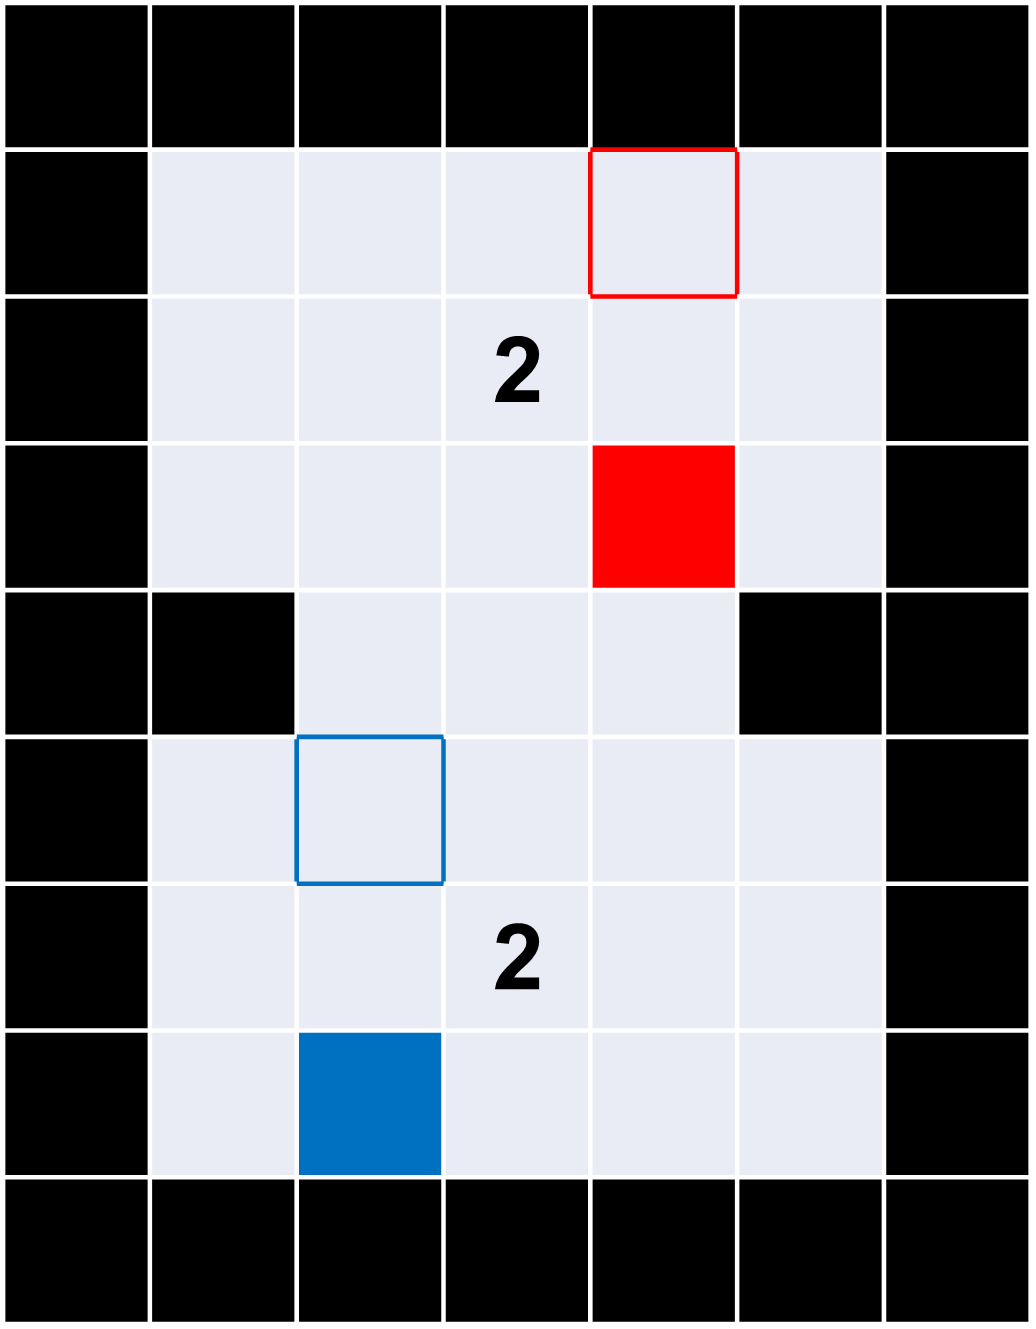
\includegraphics[width=0.1\textwidth]{Images/P1s.png}
%         \label{subfig:s1}} 
%     \subfigure[$S_2$]{
%         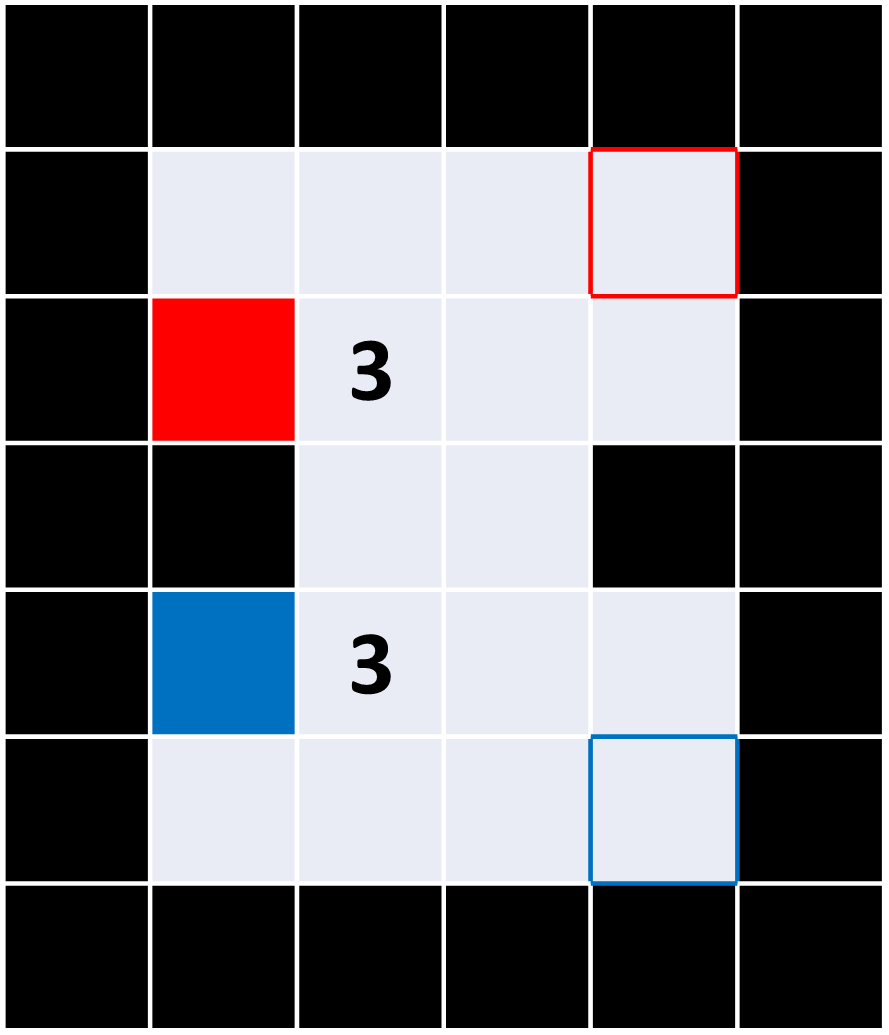
\includegraphics[width=0.11\textwidth]{Images/P2s.png}
%         \label{subfig:s2}} 
%     \subfigure[$S_3$]{
%         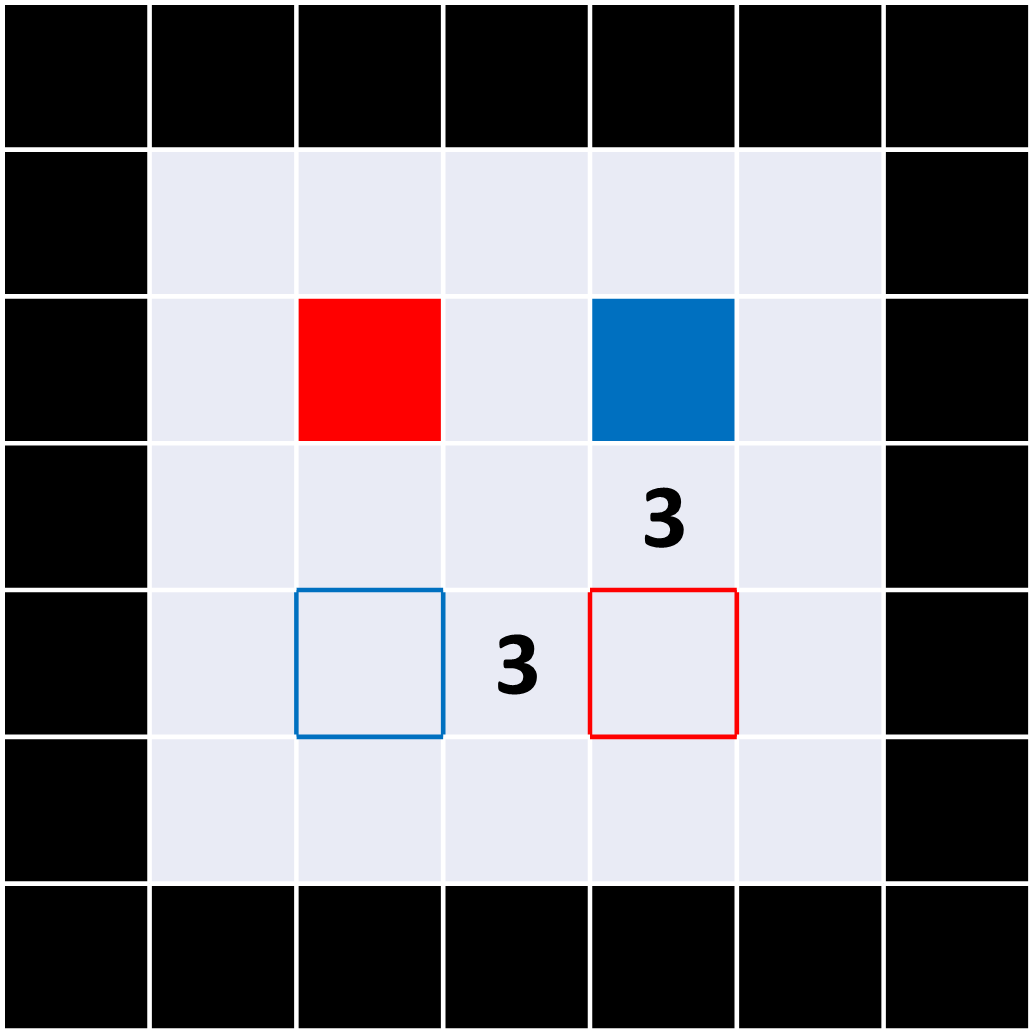
\includegraphics[width=0.13\textwidth]{Images/P3s.png}
%         \label{subfig:s3}}
%     \subfigure[$S_4$]{
%         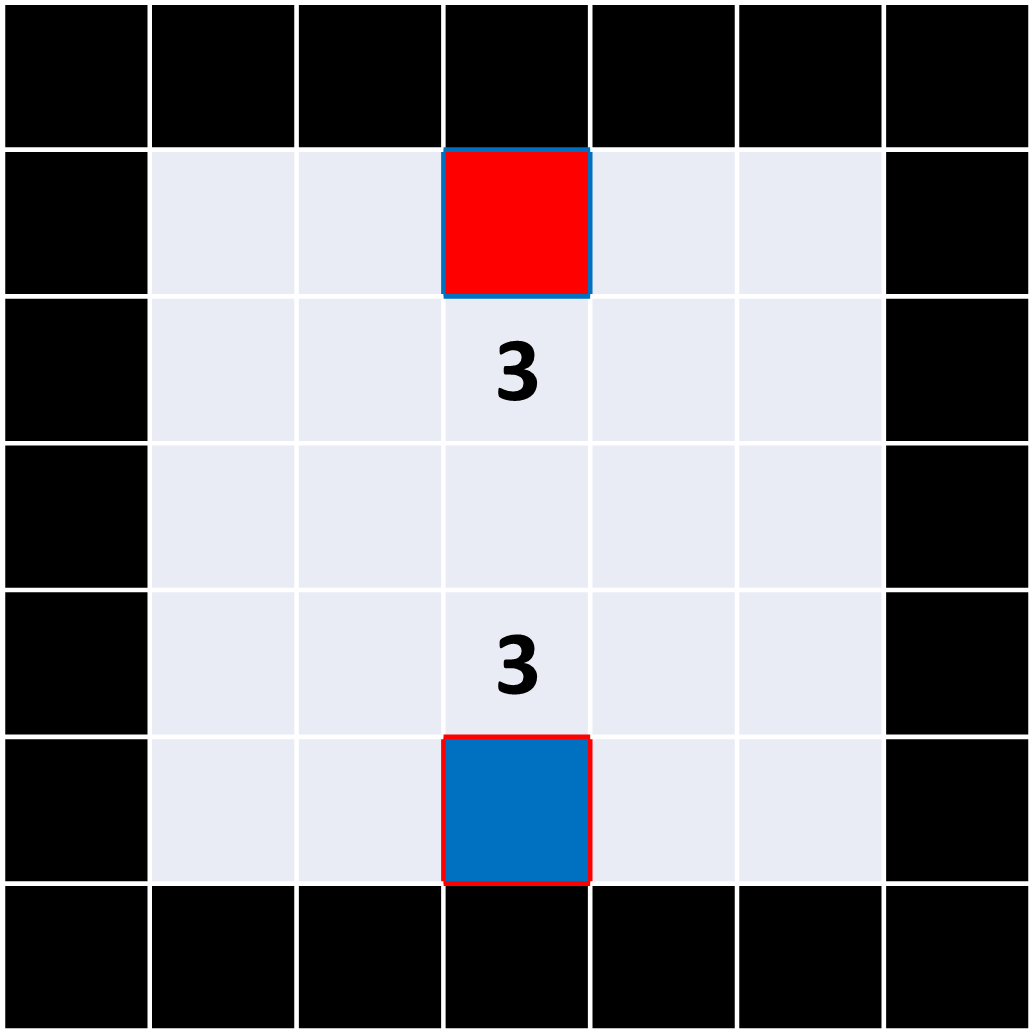
\includegraphics[width=0.13\textwidth]{Images/P4s.png}
%         \label{subfig:$S_4$}}
% %    \caption{2 agents' smaller benchmarks, used to compare our algorithm to a joint offline version.}
% %    \label{fig:small-problems}
% %\end{figure}
% % \begin{figure}[ht]
% \subfigure[$M_1$]{
%         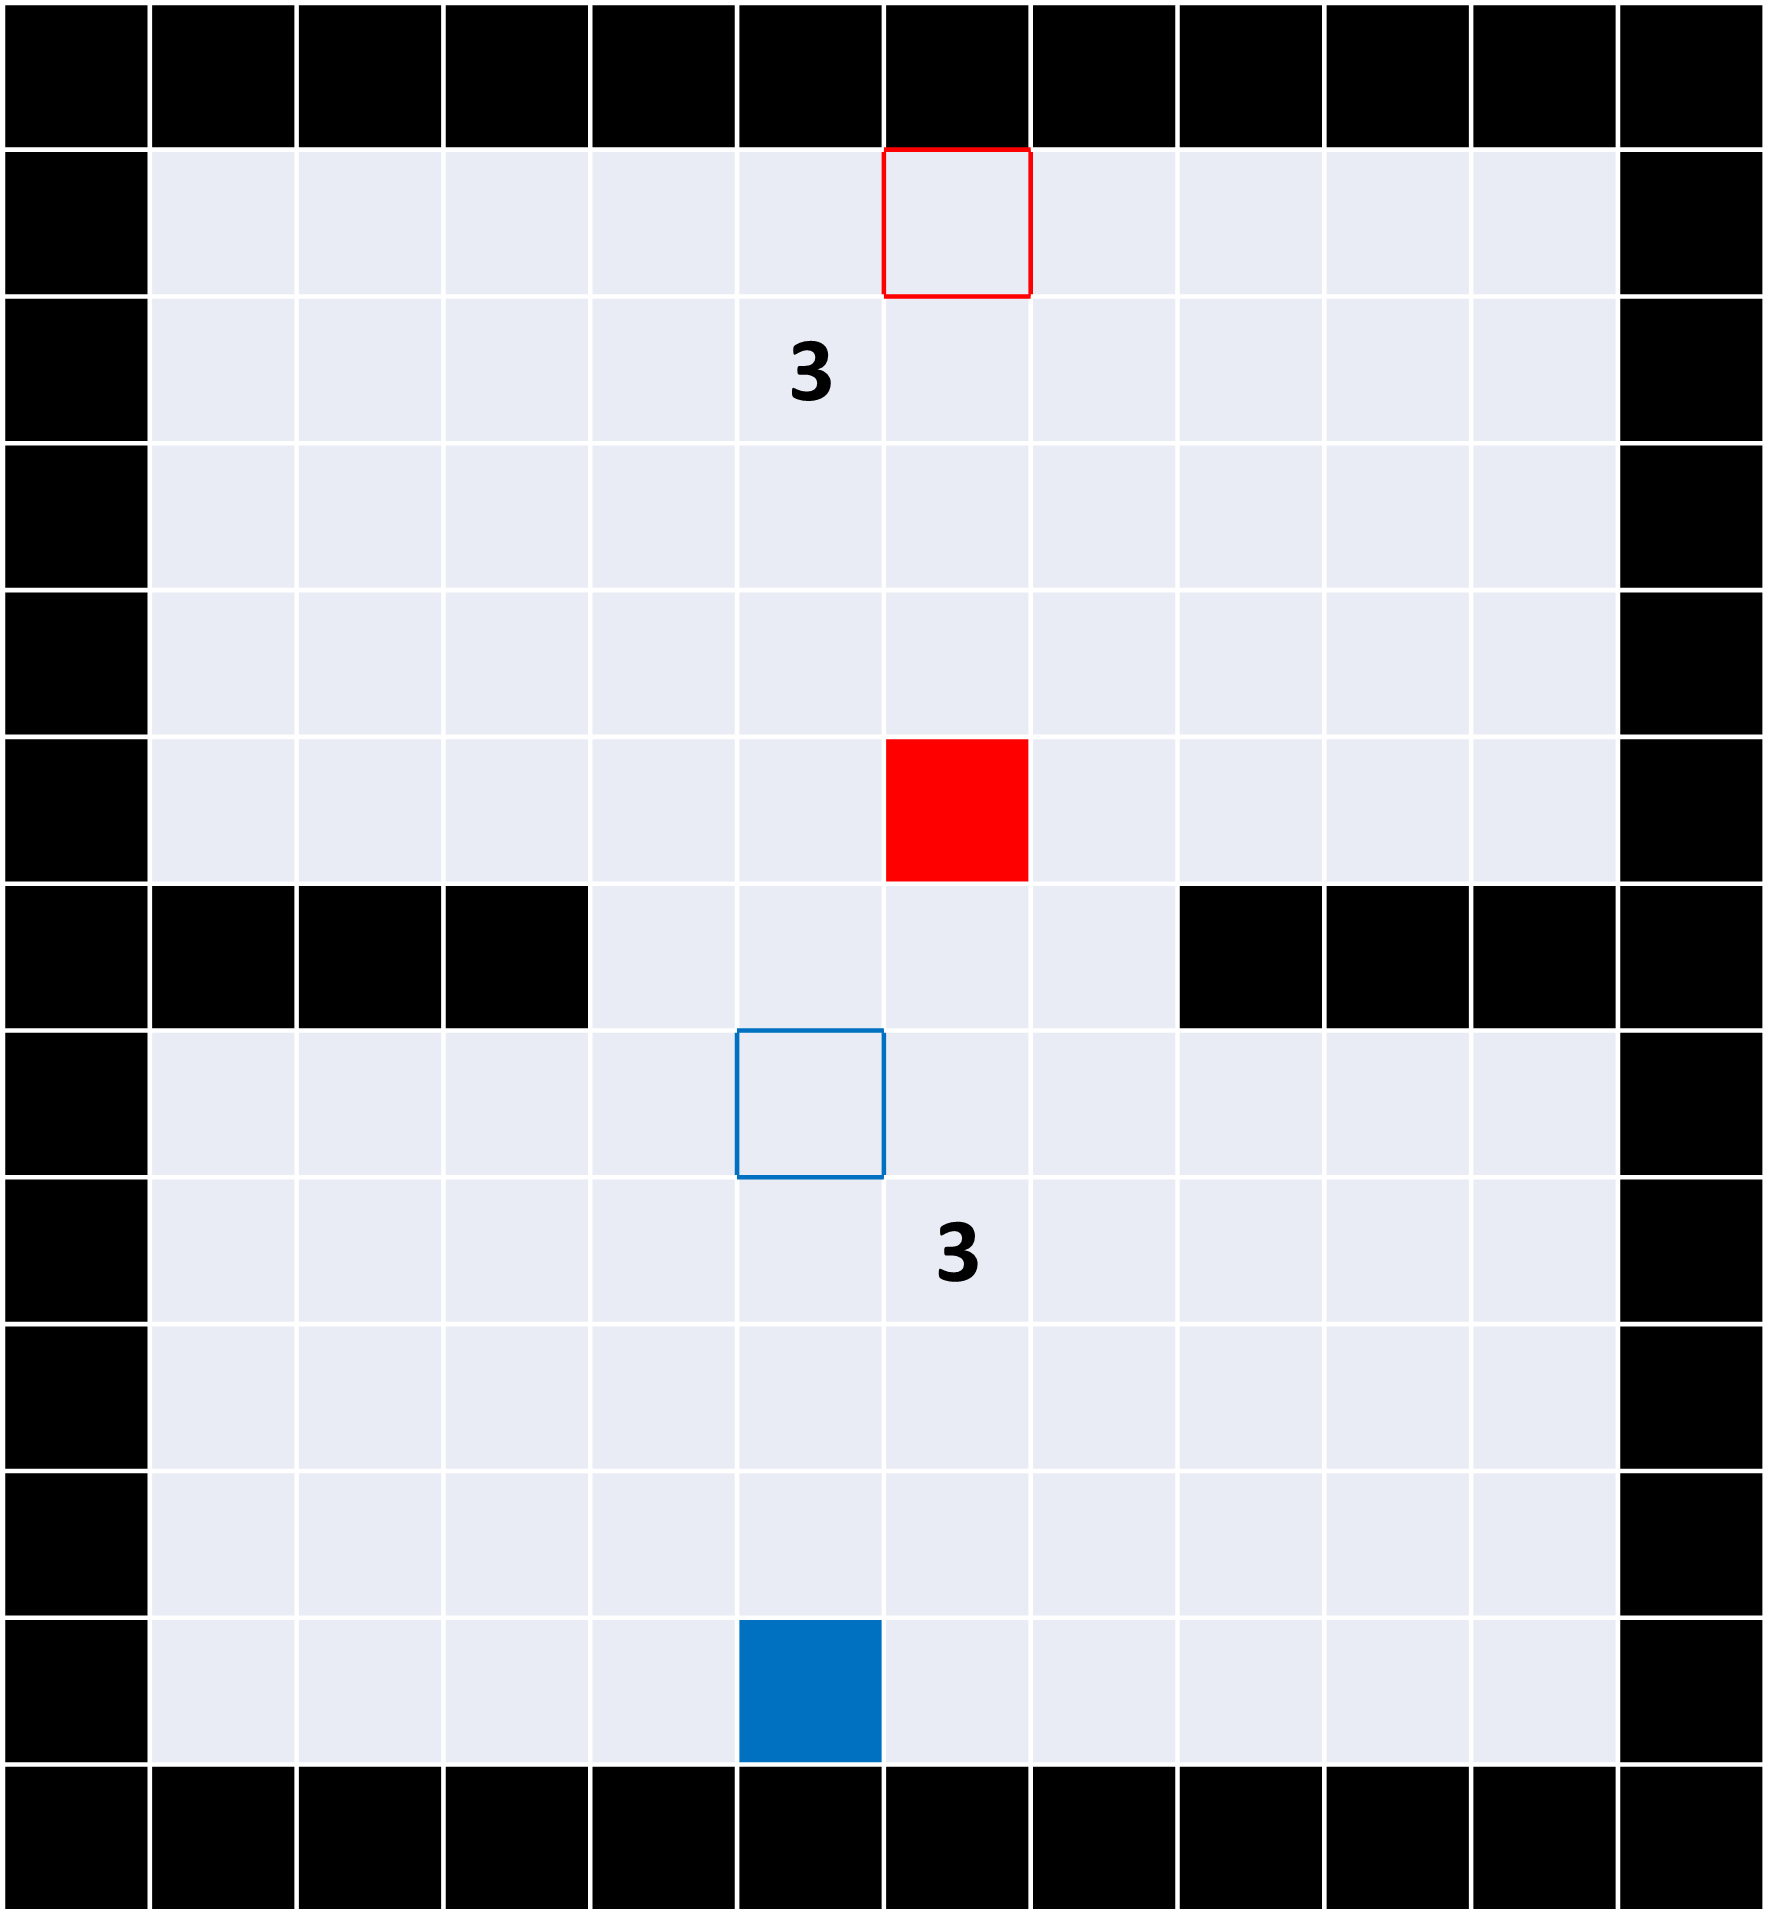
\includegraphics[width=0.12\textwidth]{Images/P1.png}
%         \label{subfig:m1}} 
%     \subfigure[$M_2$]{
%         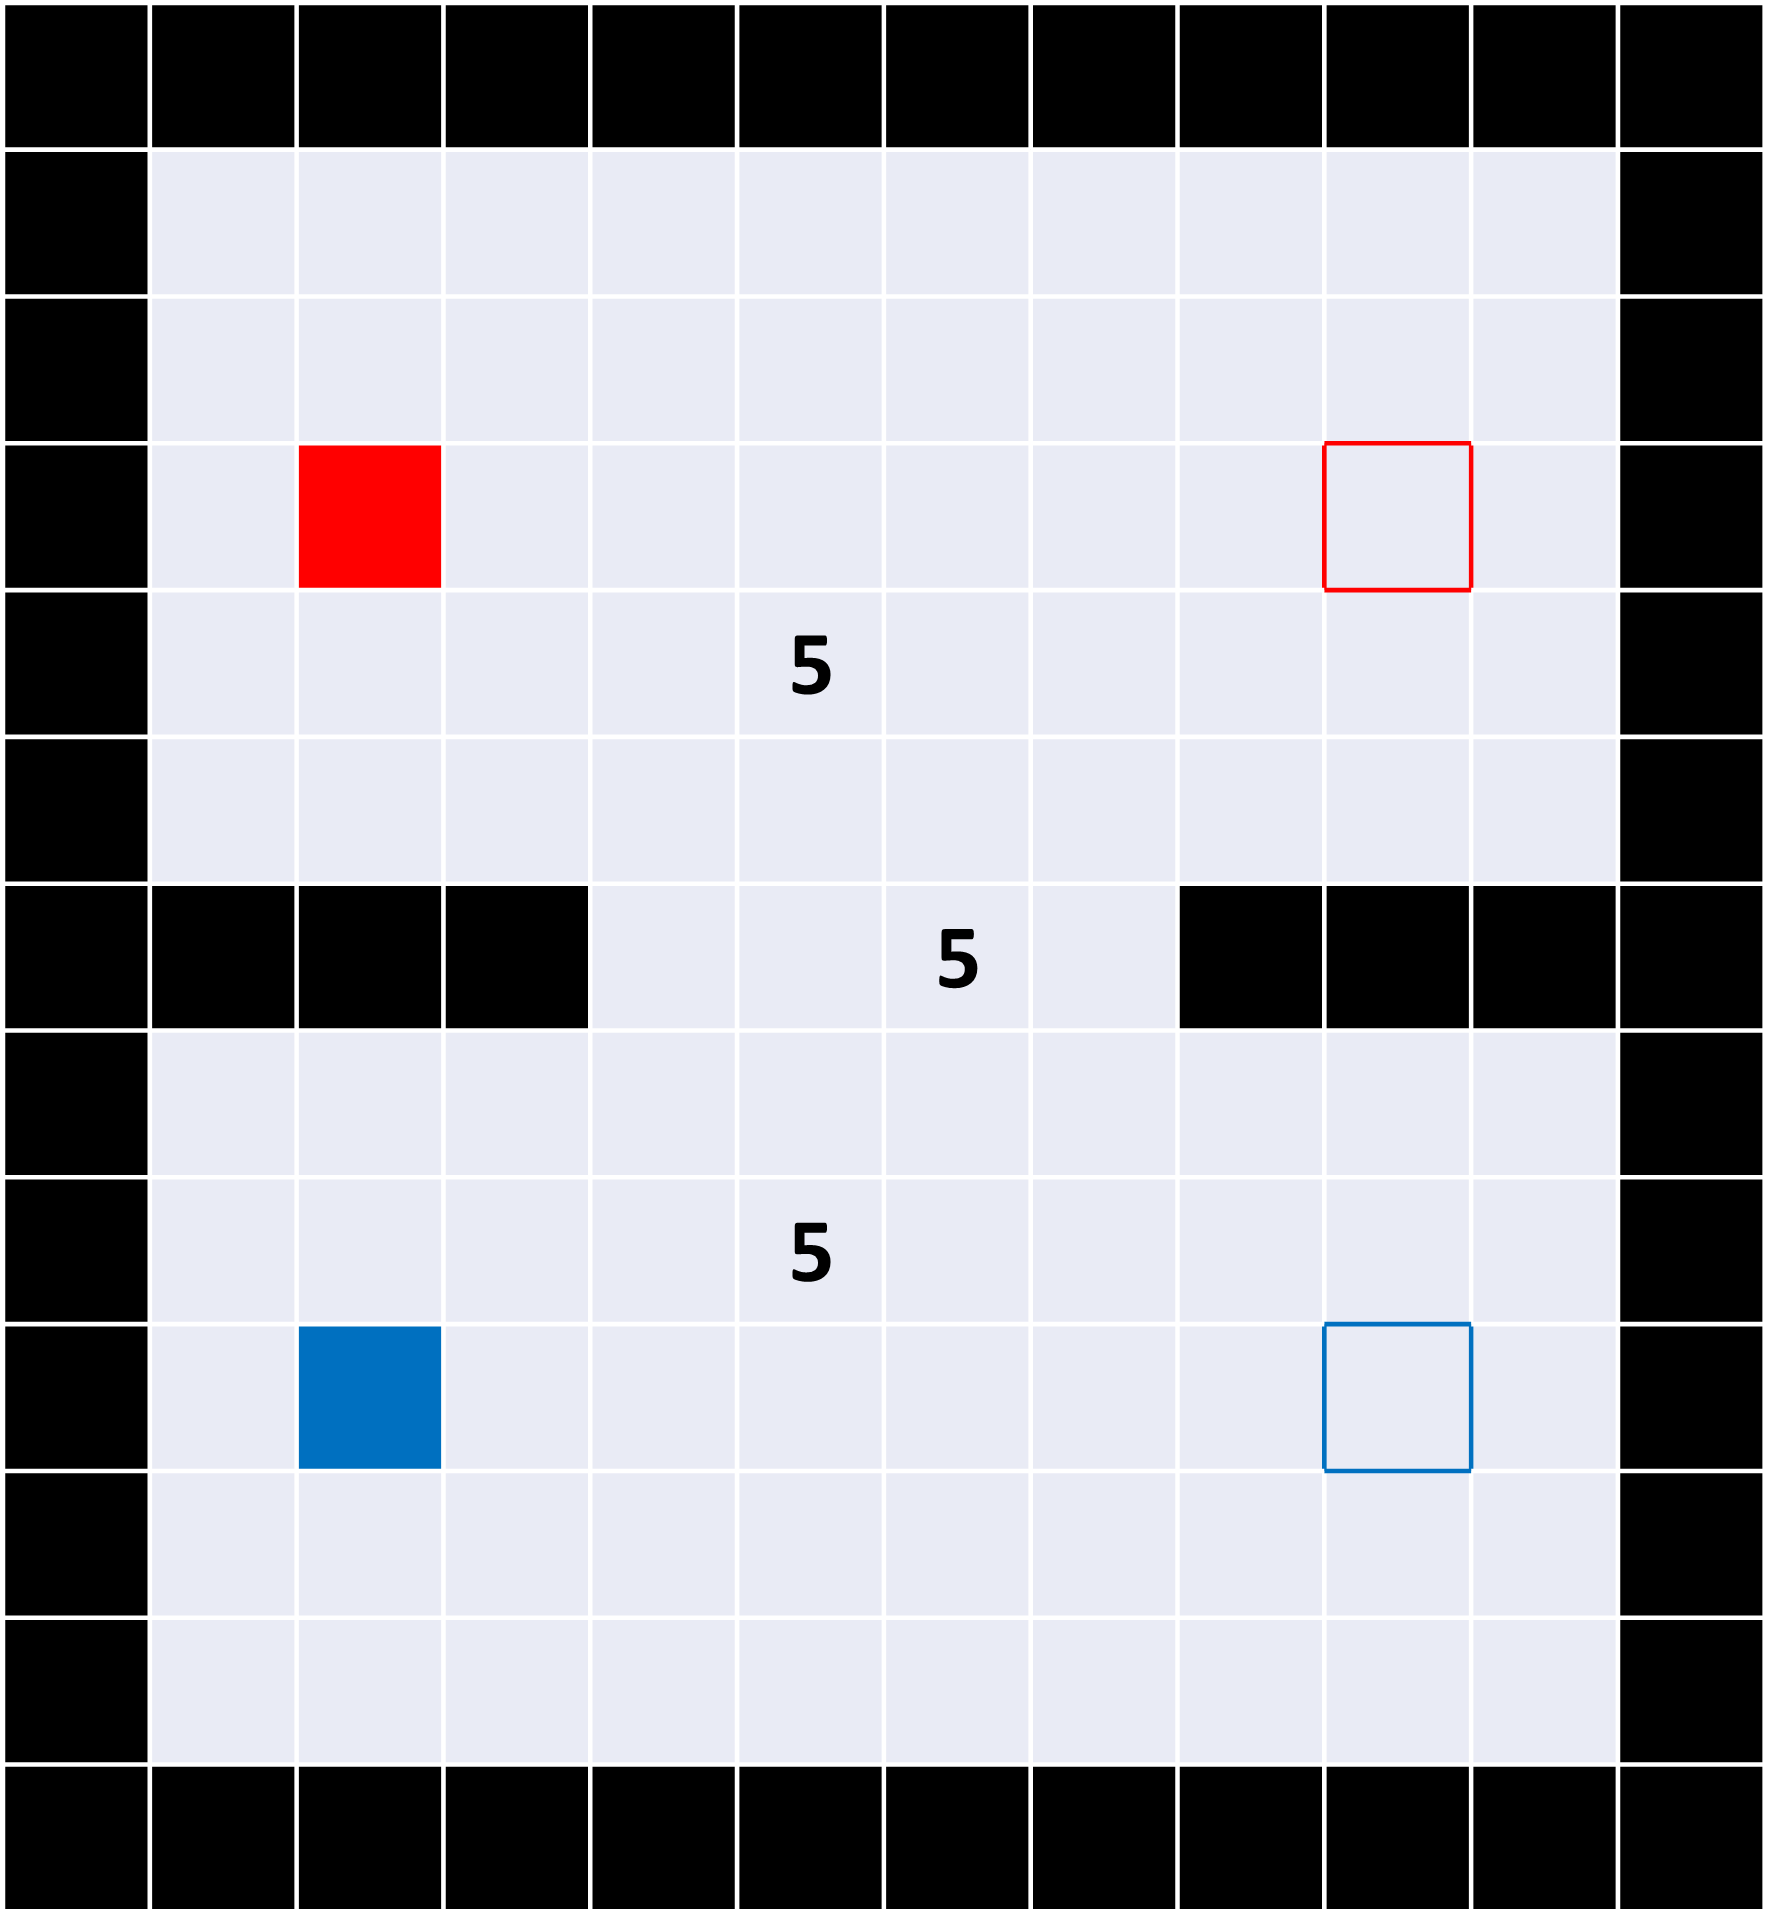
\includegraphics[width=0.12\textwidth]{Images/P2.png}
%         \label{subfig:m2}} 
%     \subfigure[$M_3$]{
%         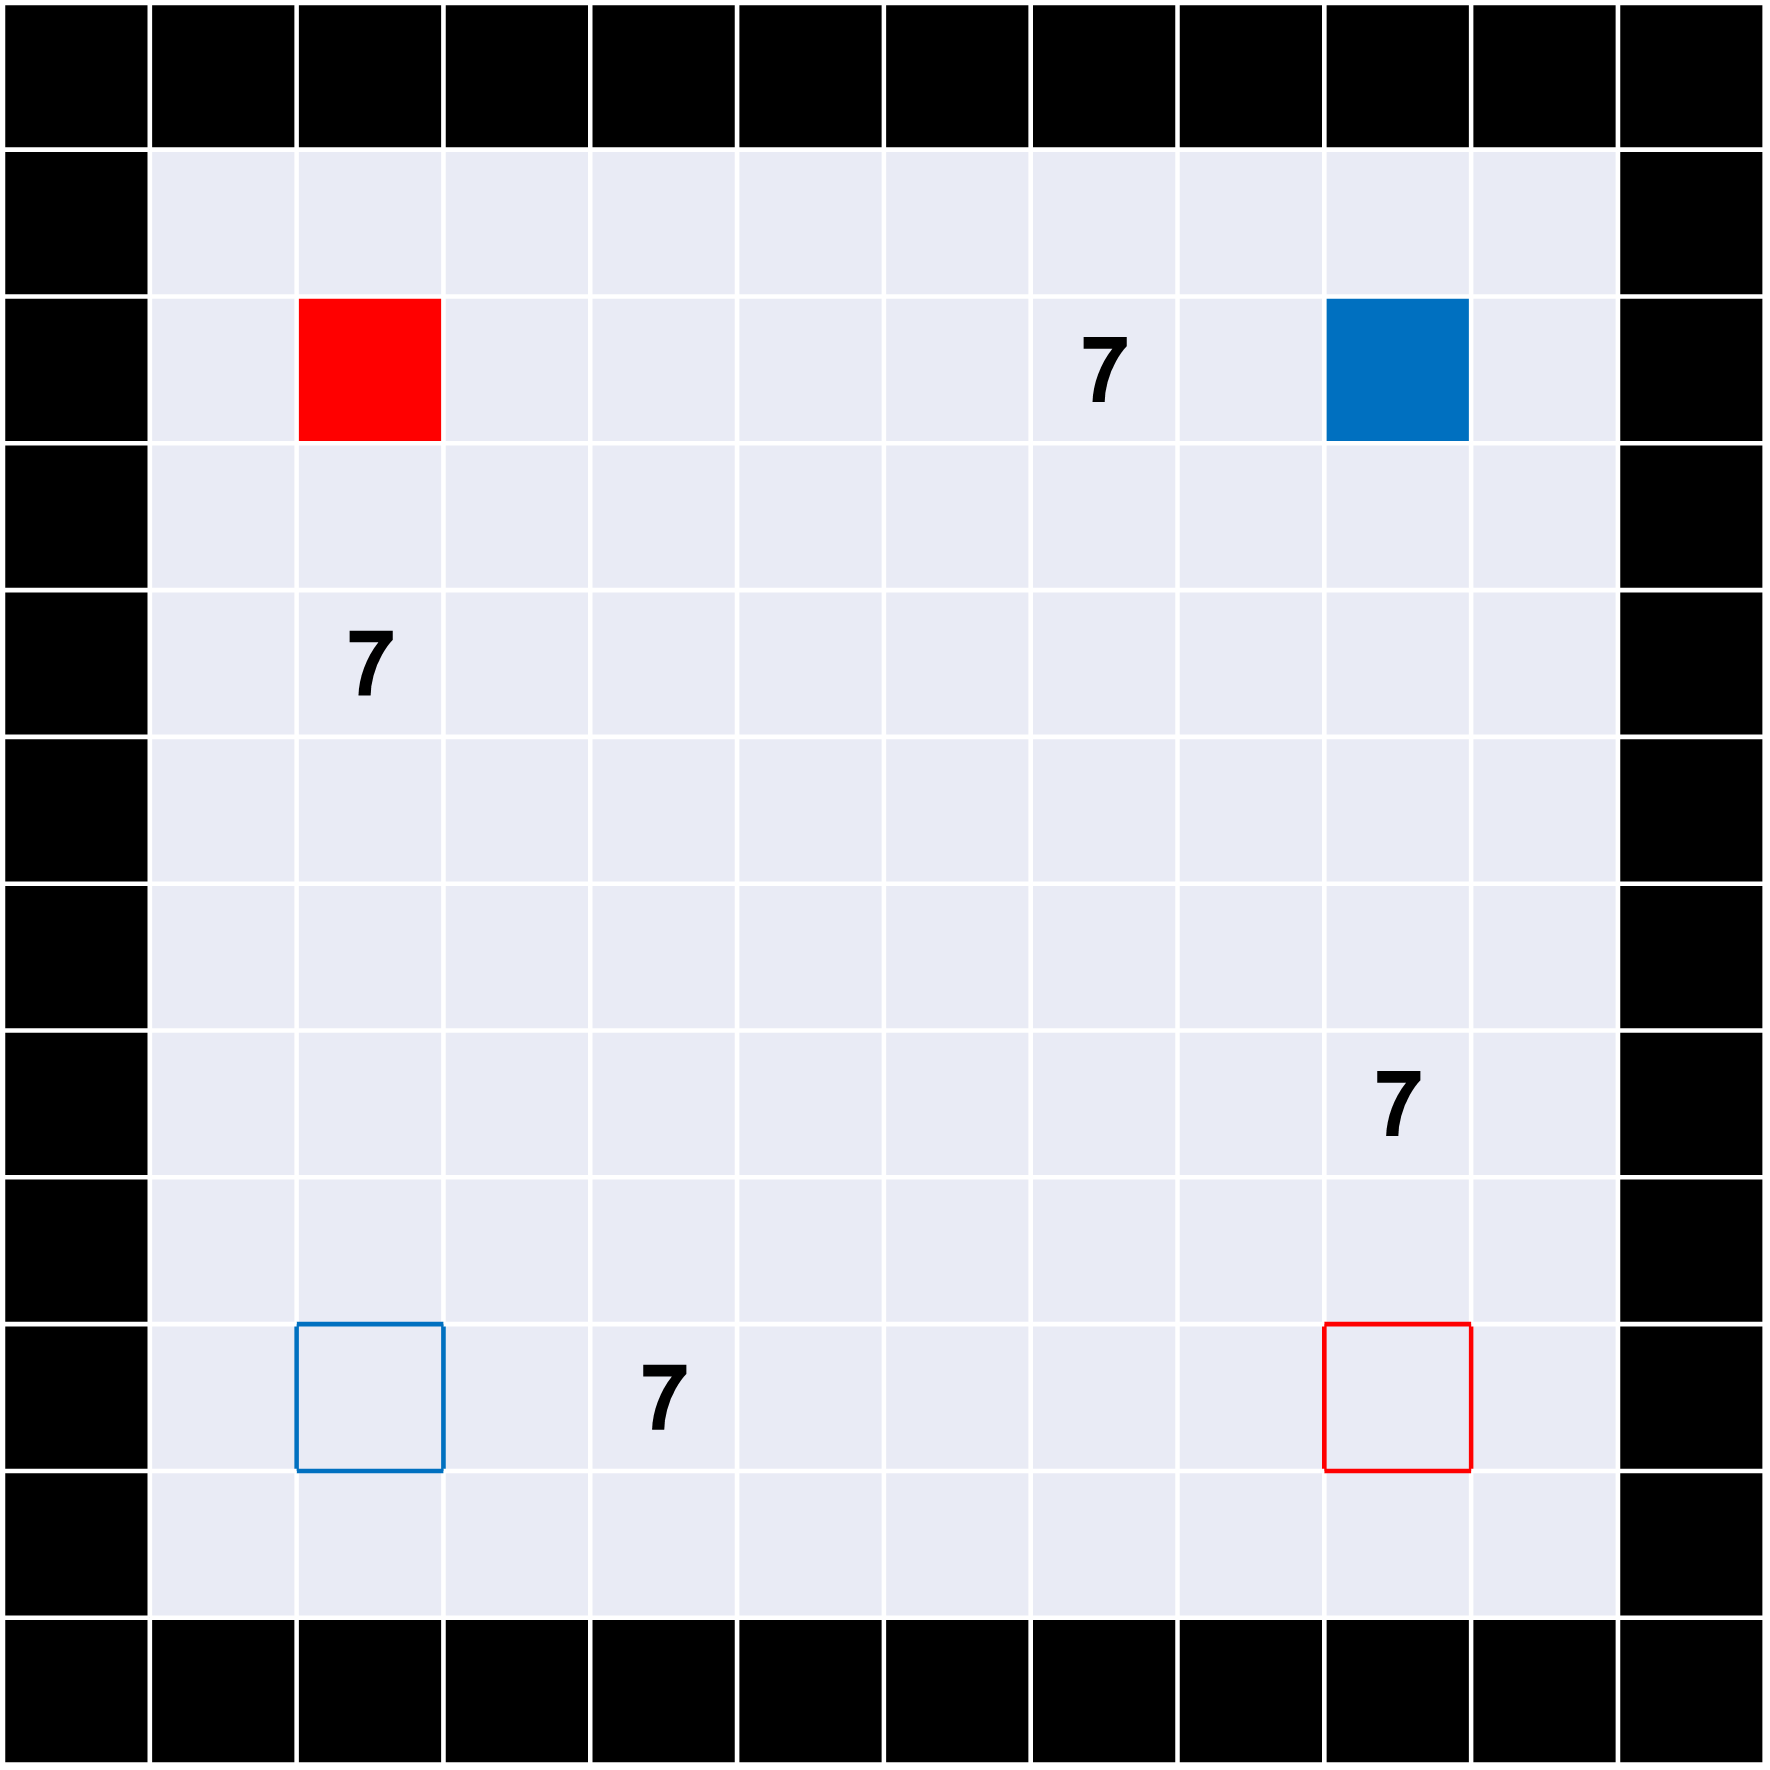
\includegraphics[width=0.13\textwidth]{Images/P3.png}
%         \label{subfig:m3}}
%     \subfigure[$M_4$]{
%         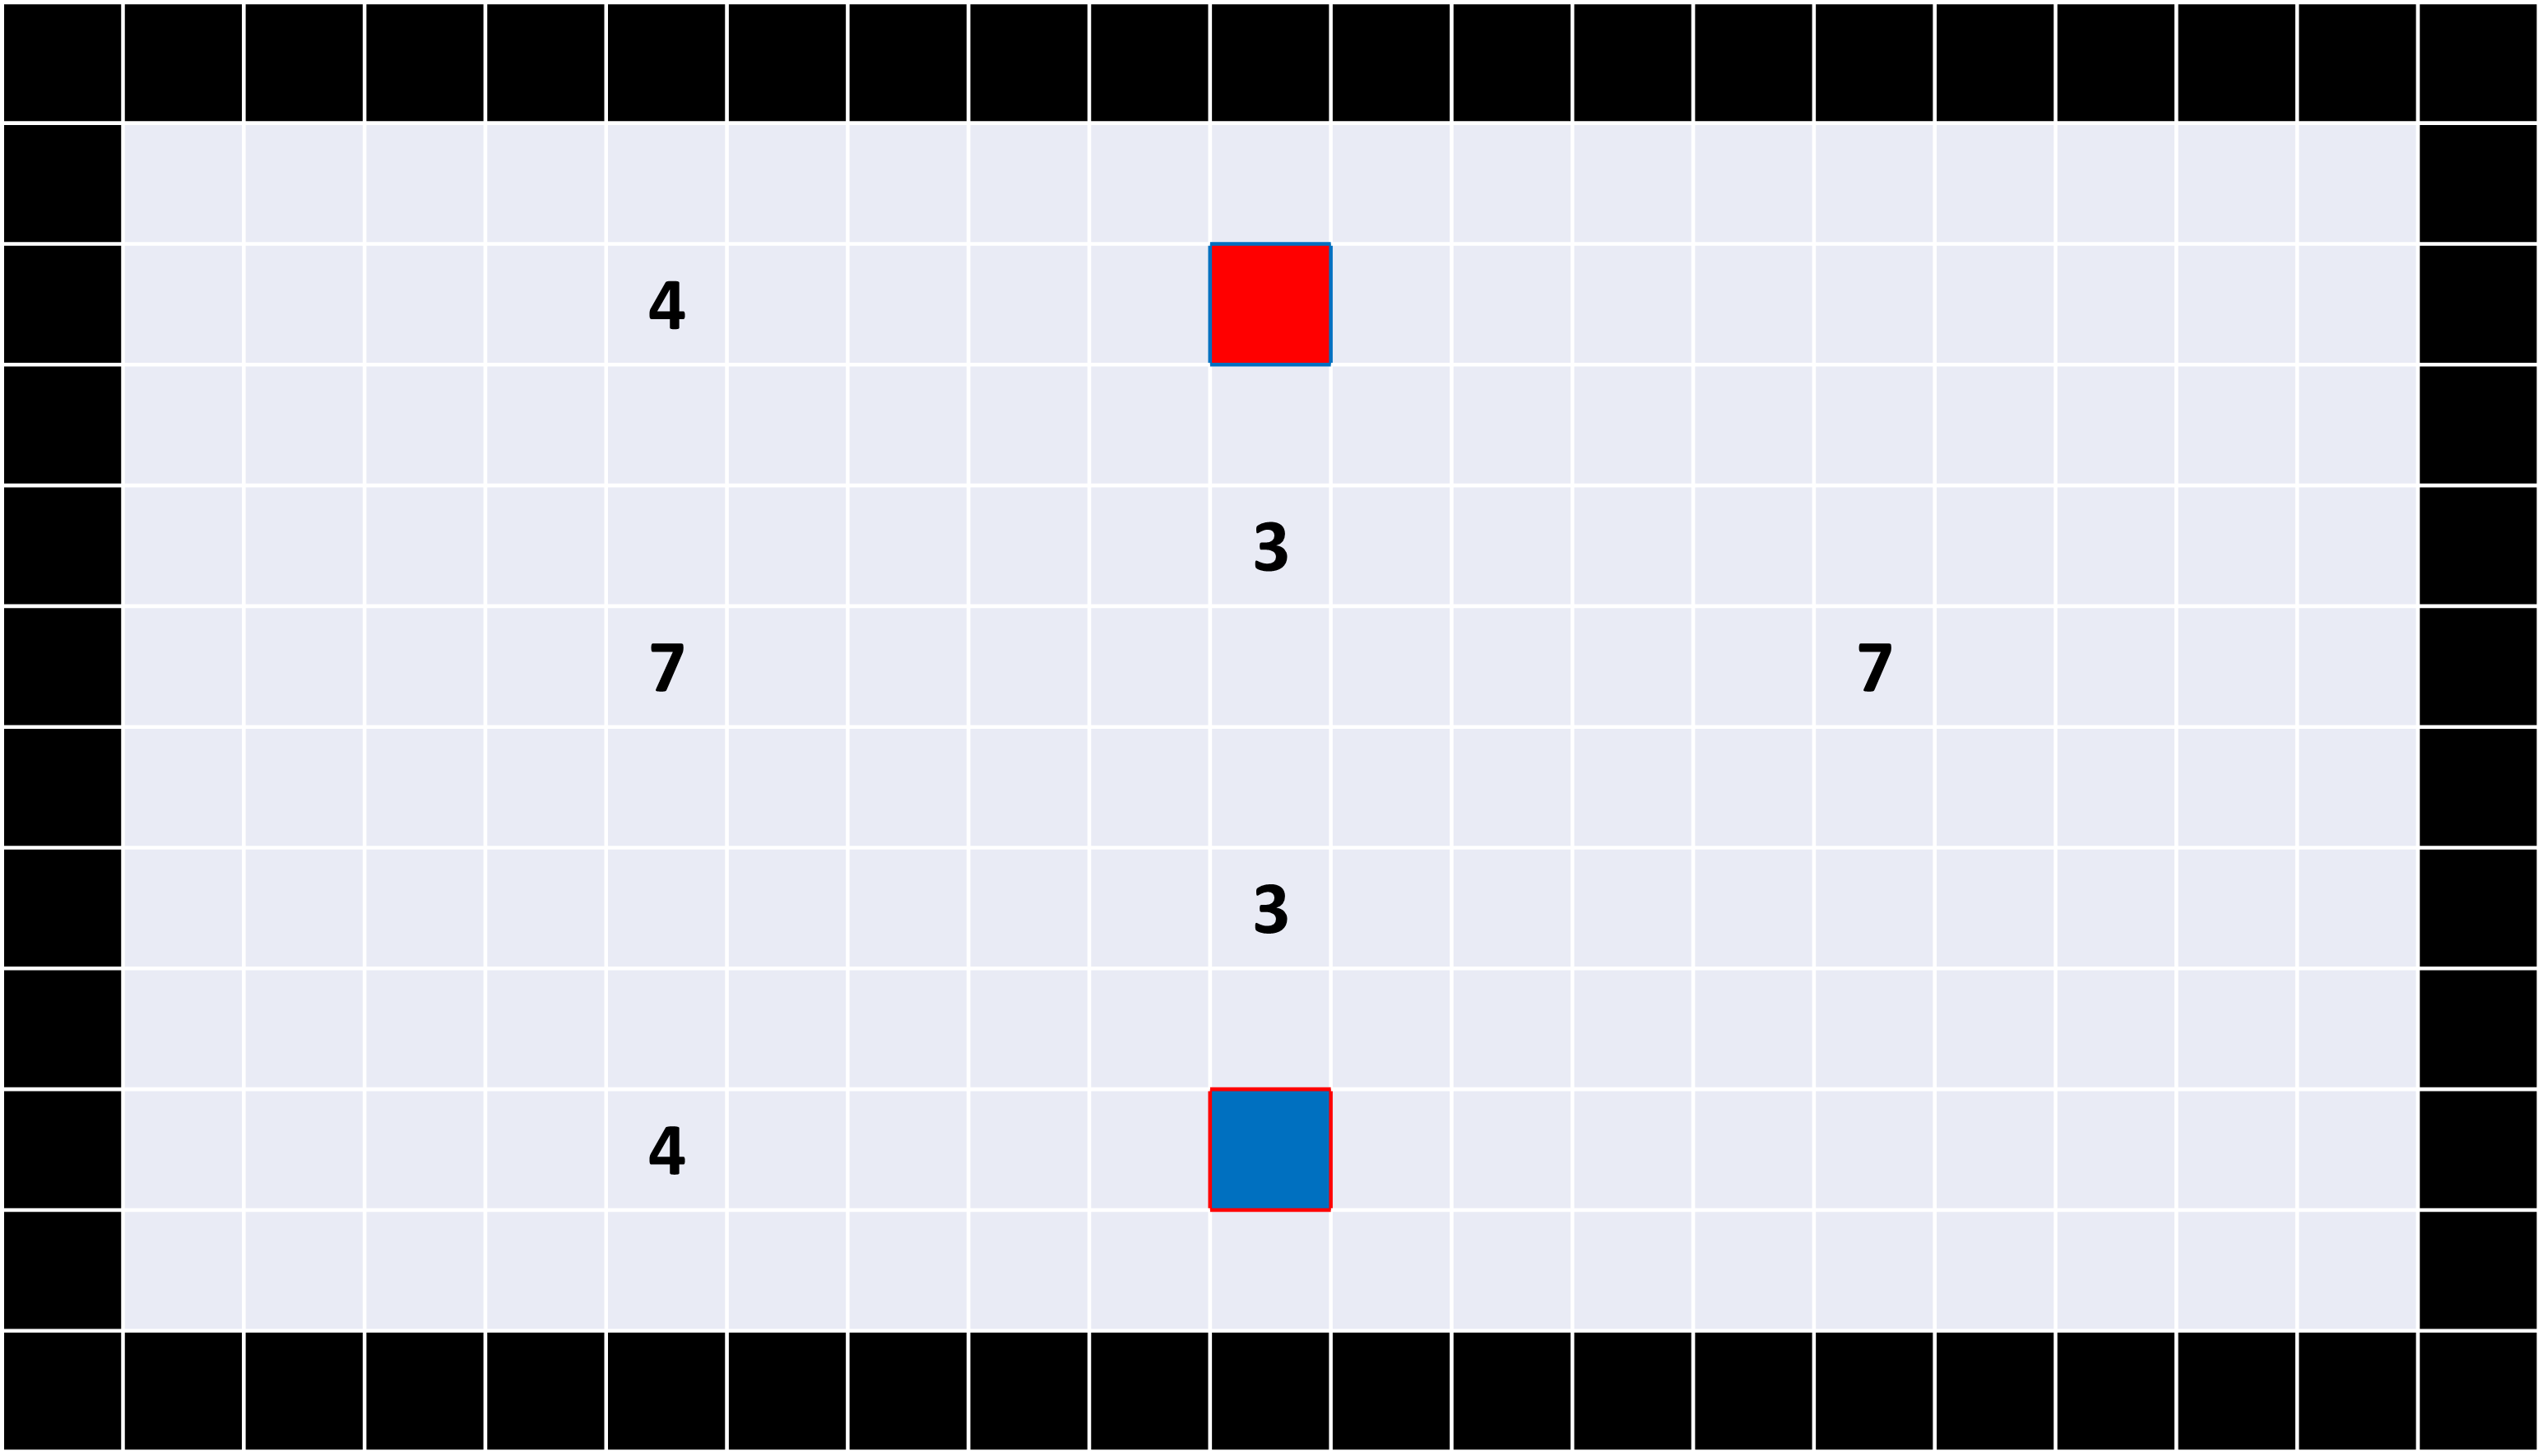
\includegraphics[width=0.245\textwidth]{Images/P4.png}
%         \label{subfig:m4}}
%     \subfigure[$M_5$]{
%         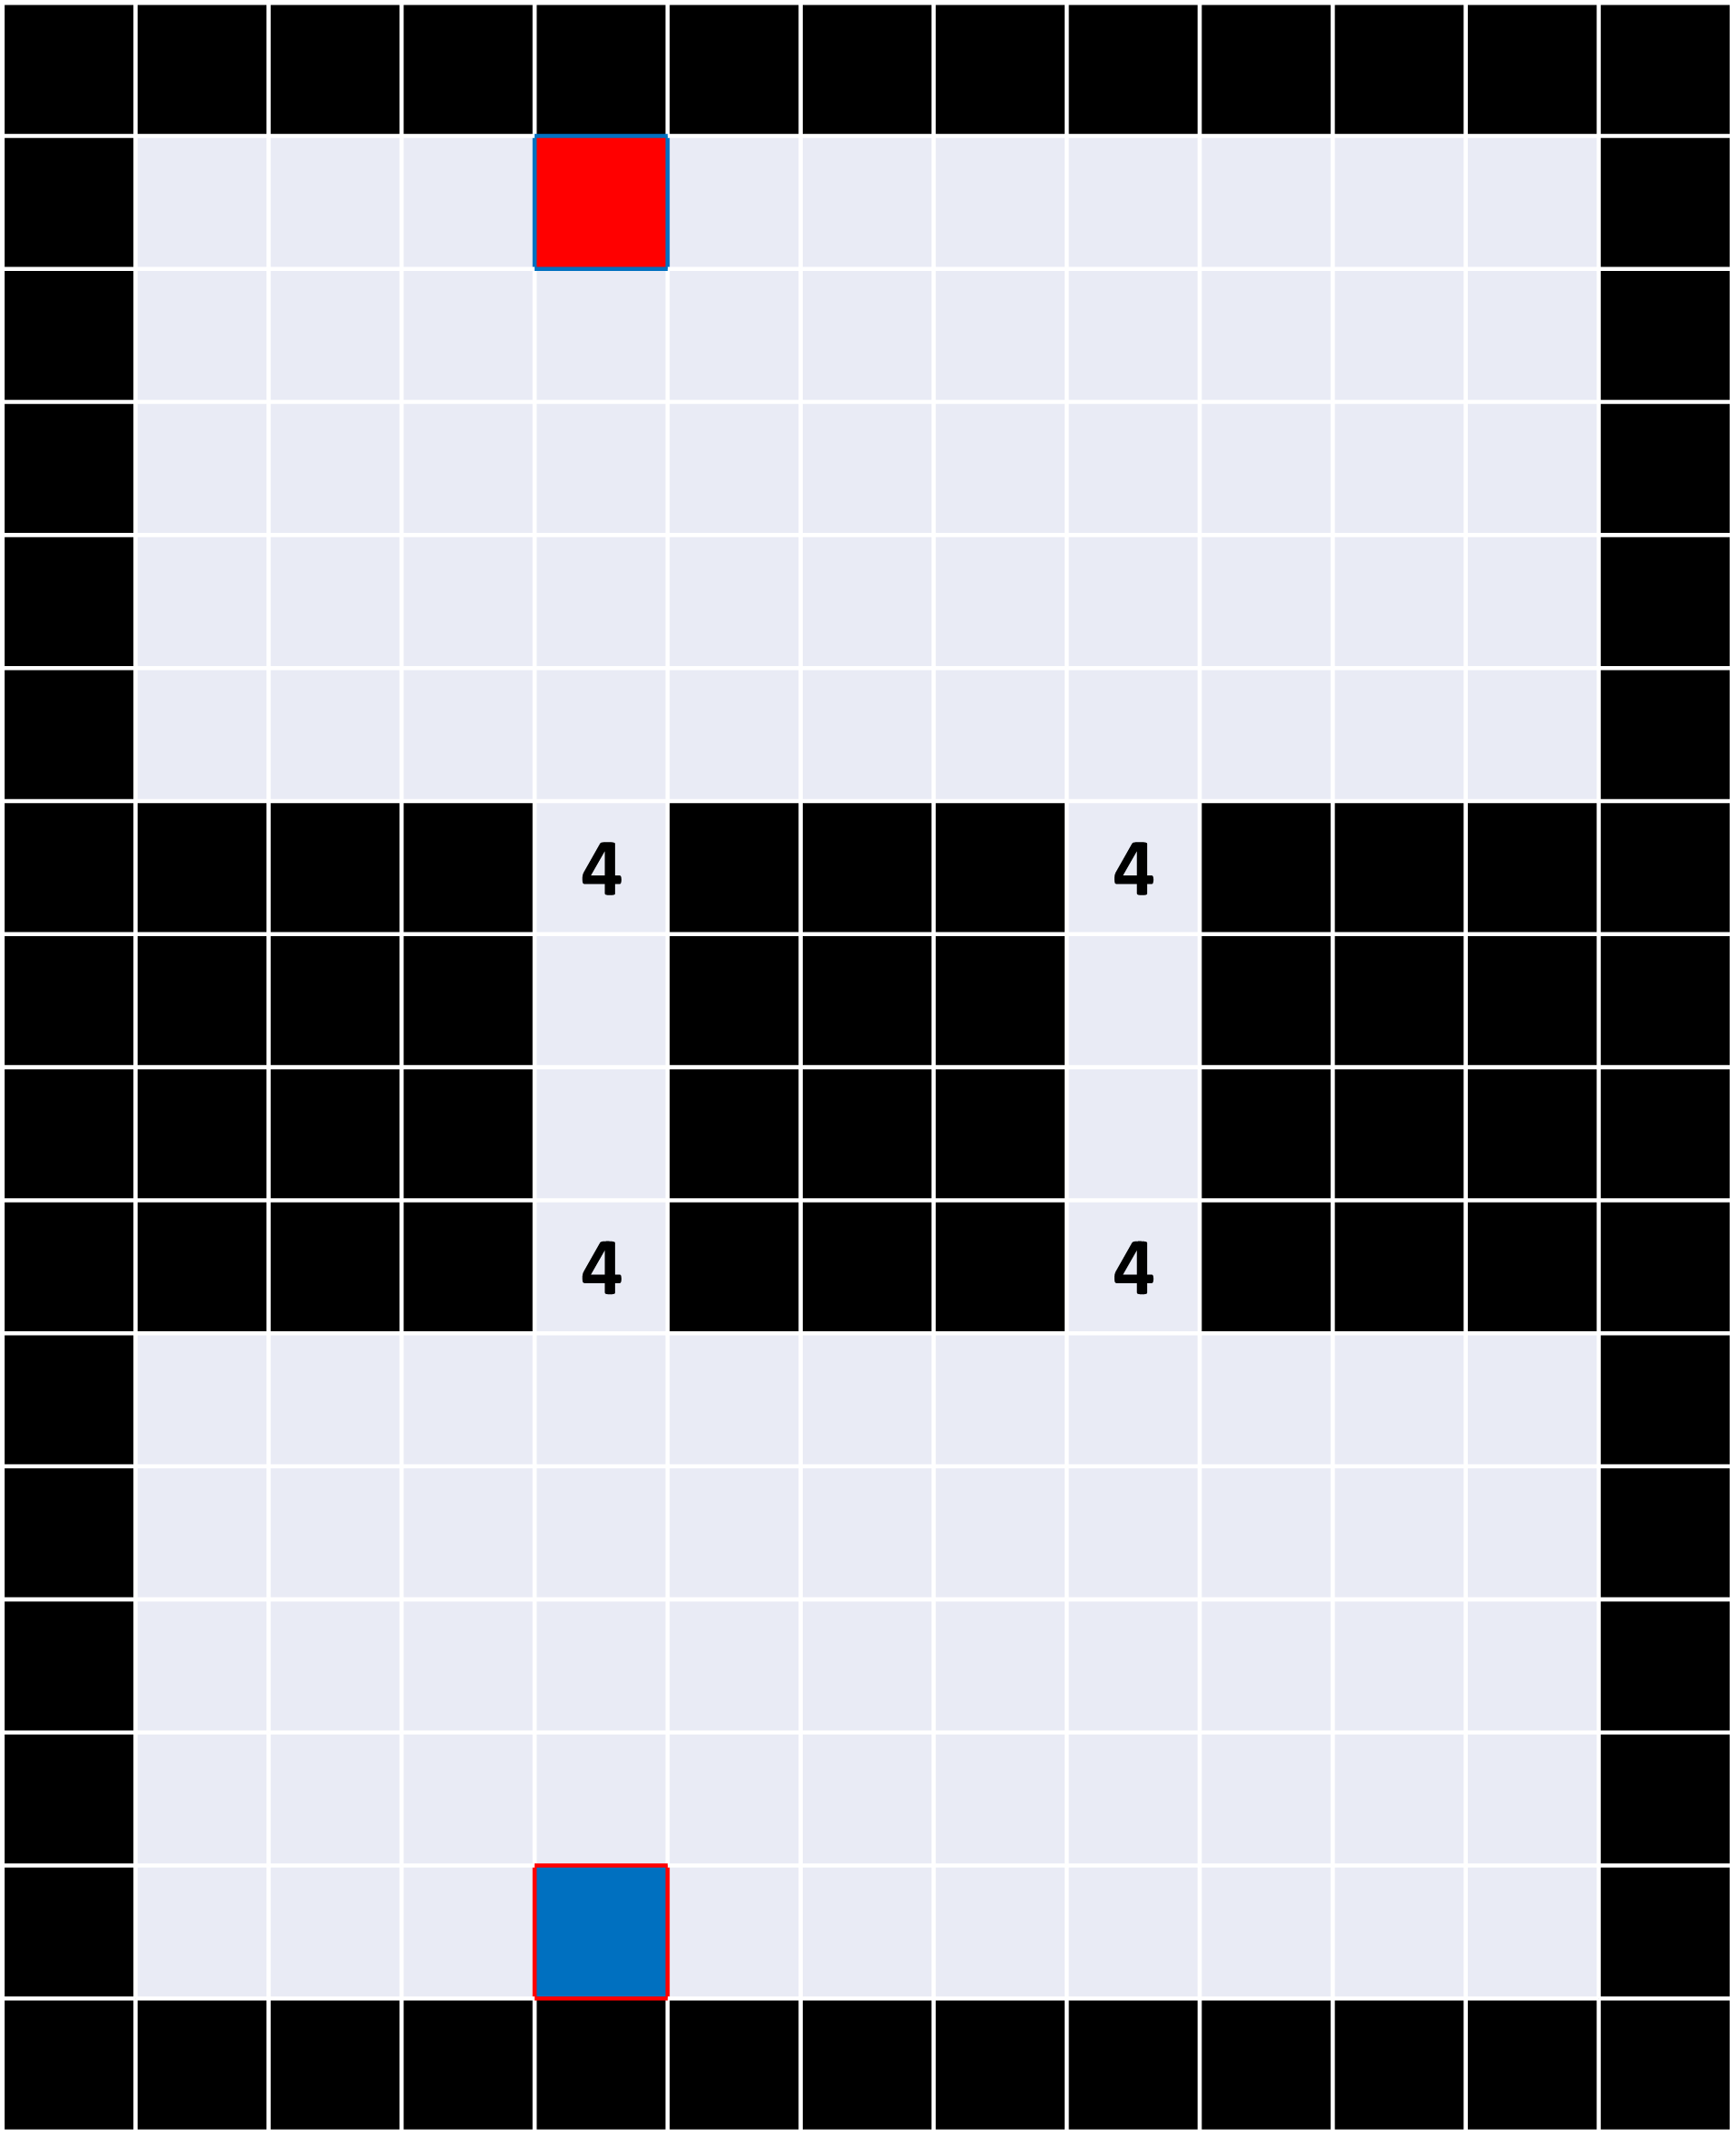
\includegraphics[width=0.115\textwidth]{Images/P5.png}
%         \label{subfig:m5}}
%     % \caption{2 agents' benchmarks used in the empirical evaluation. Each color represents an agent, where the filled cells are the agents' initial states and the bordered cells are the agents' goal states. Black cells are blocked. The numbers within cells represent beacons with respective influence range, located in those cells.}
%     % \label{fig:big-problems}
%      \subfigure[$L_1$]{
%         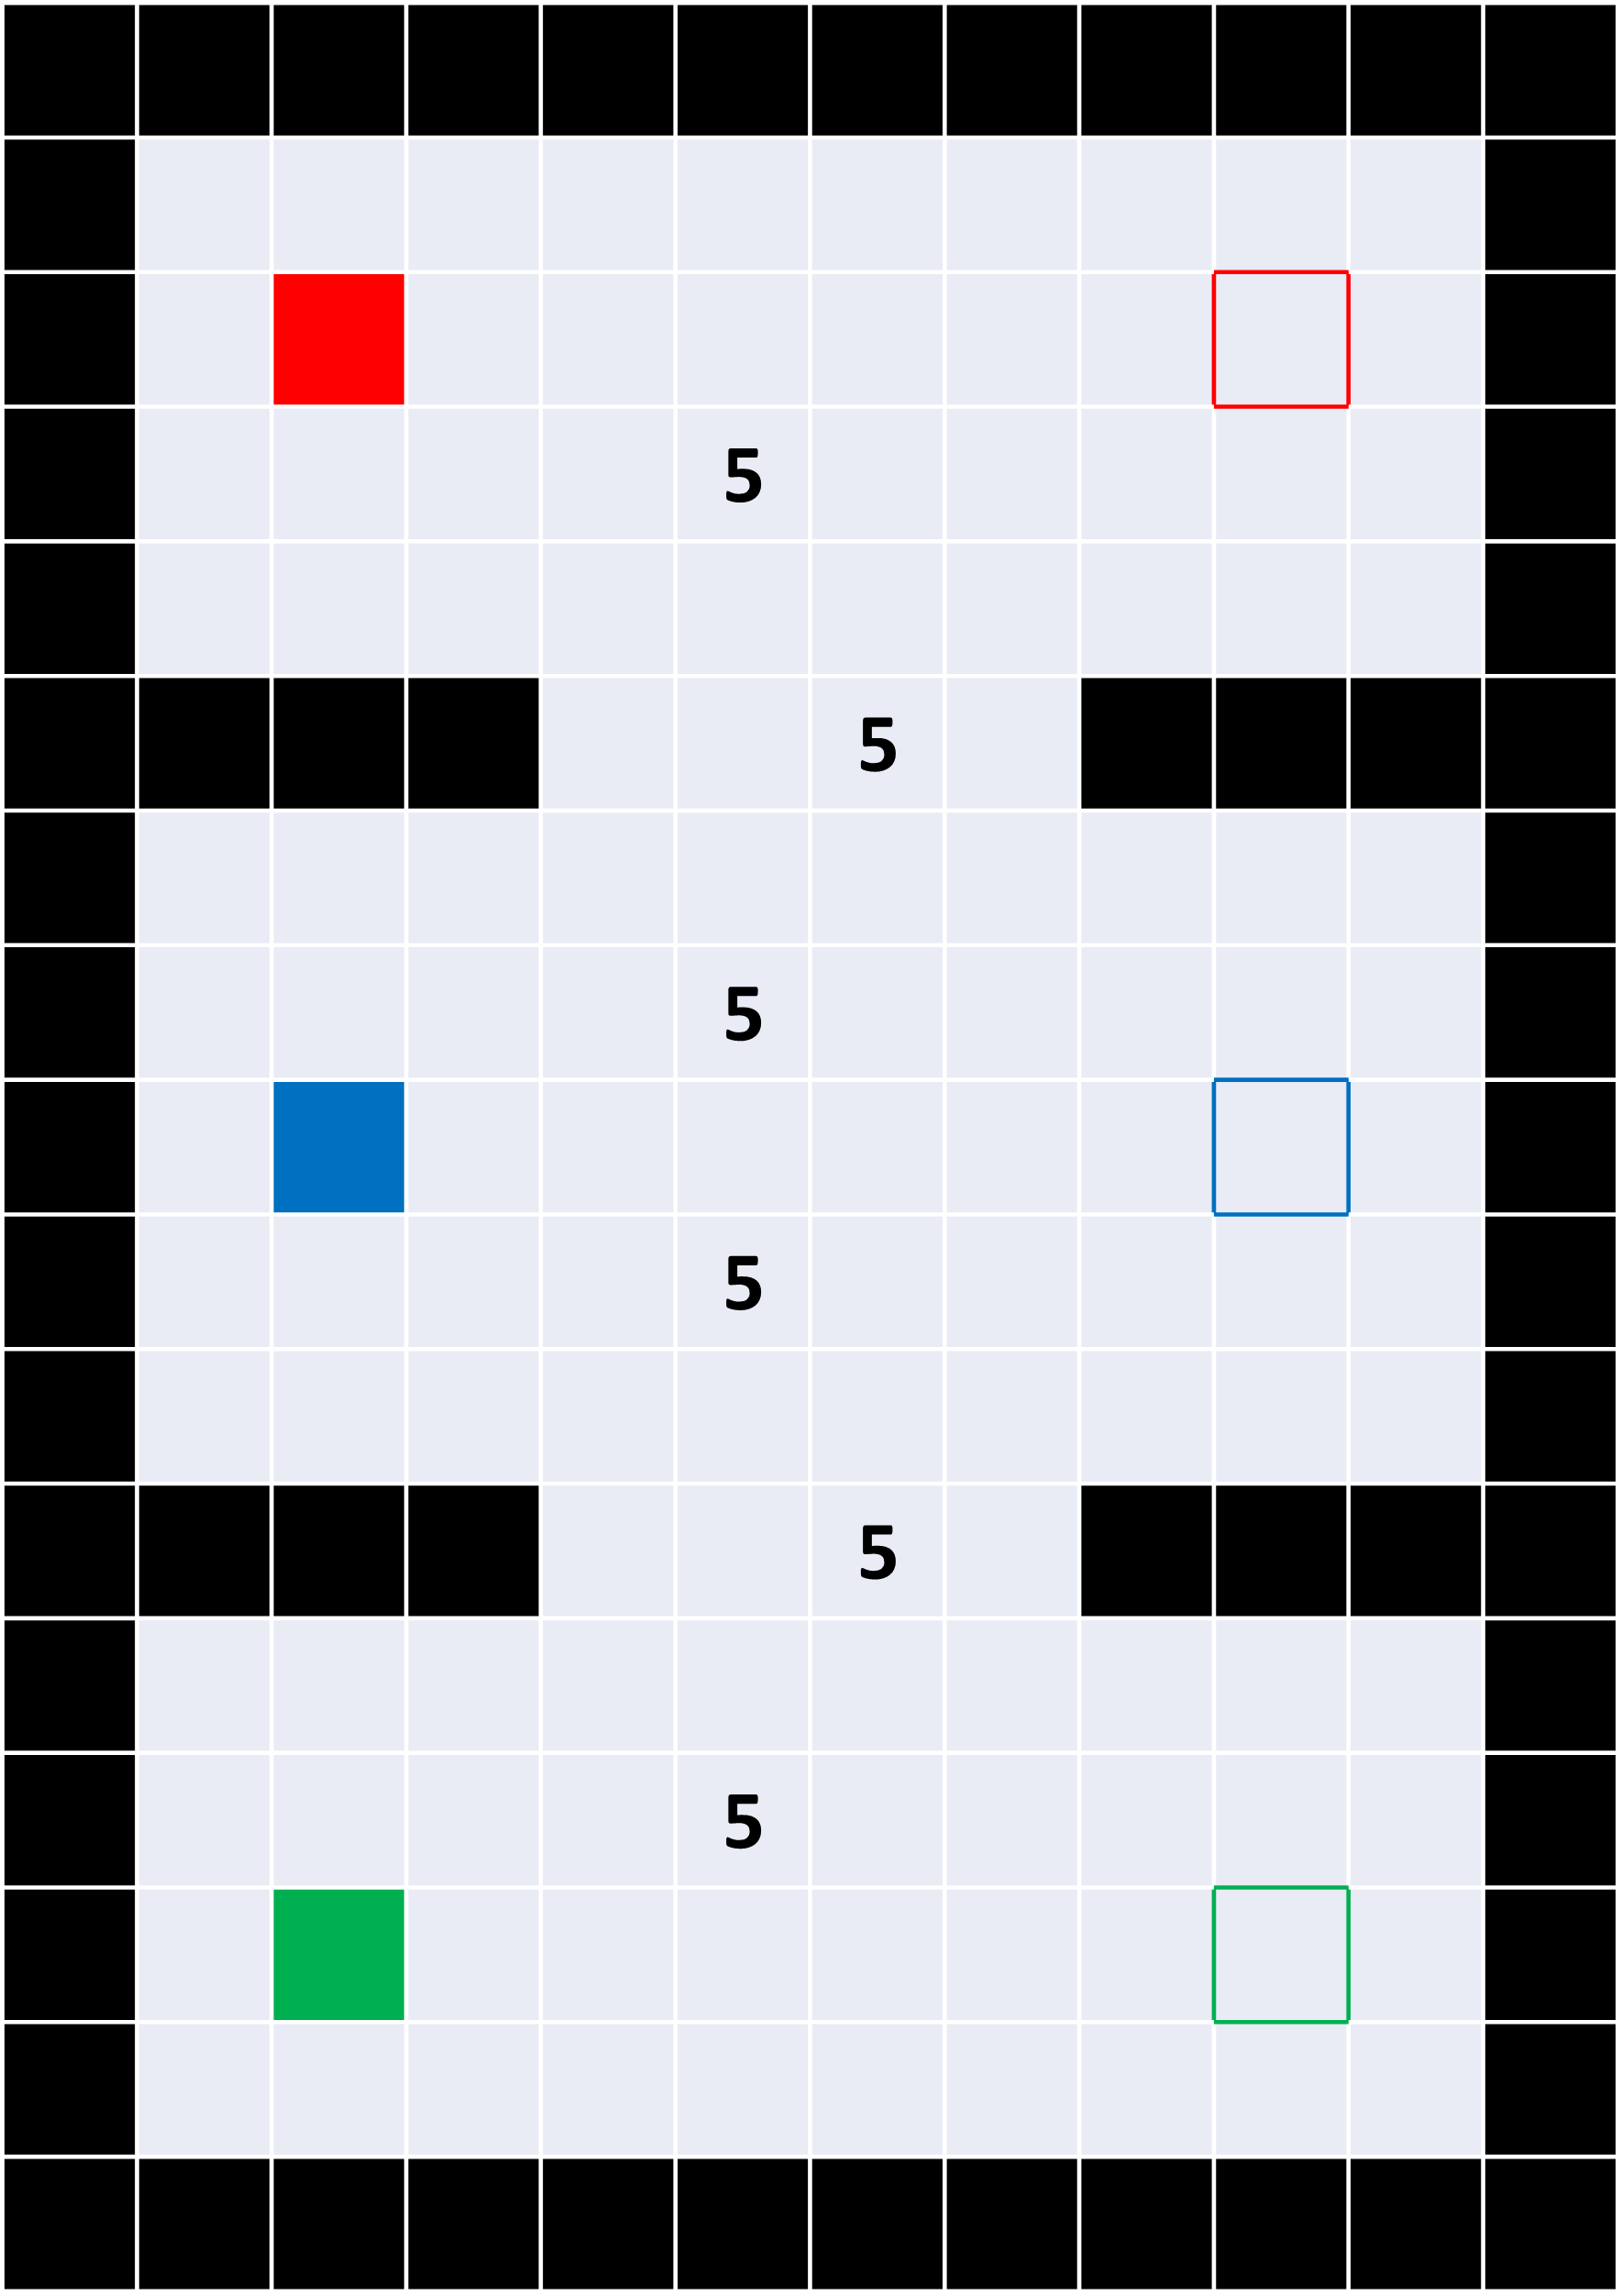
\includegraphics[width=0.1\textwidth]{Images/P2-3a.png}
%         \label{subfig:l1}}
%     \subfigure[$L_2$]{
%         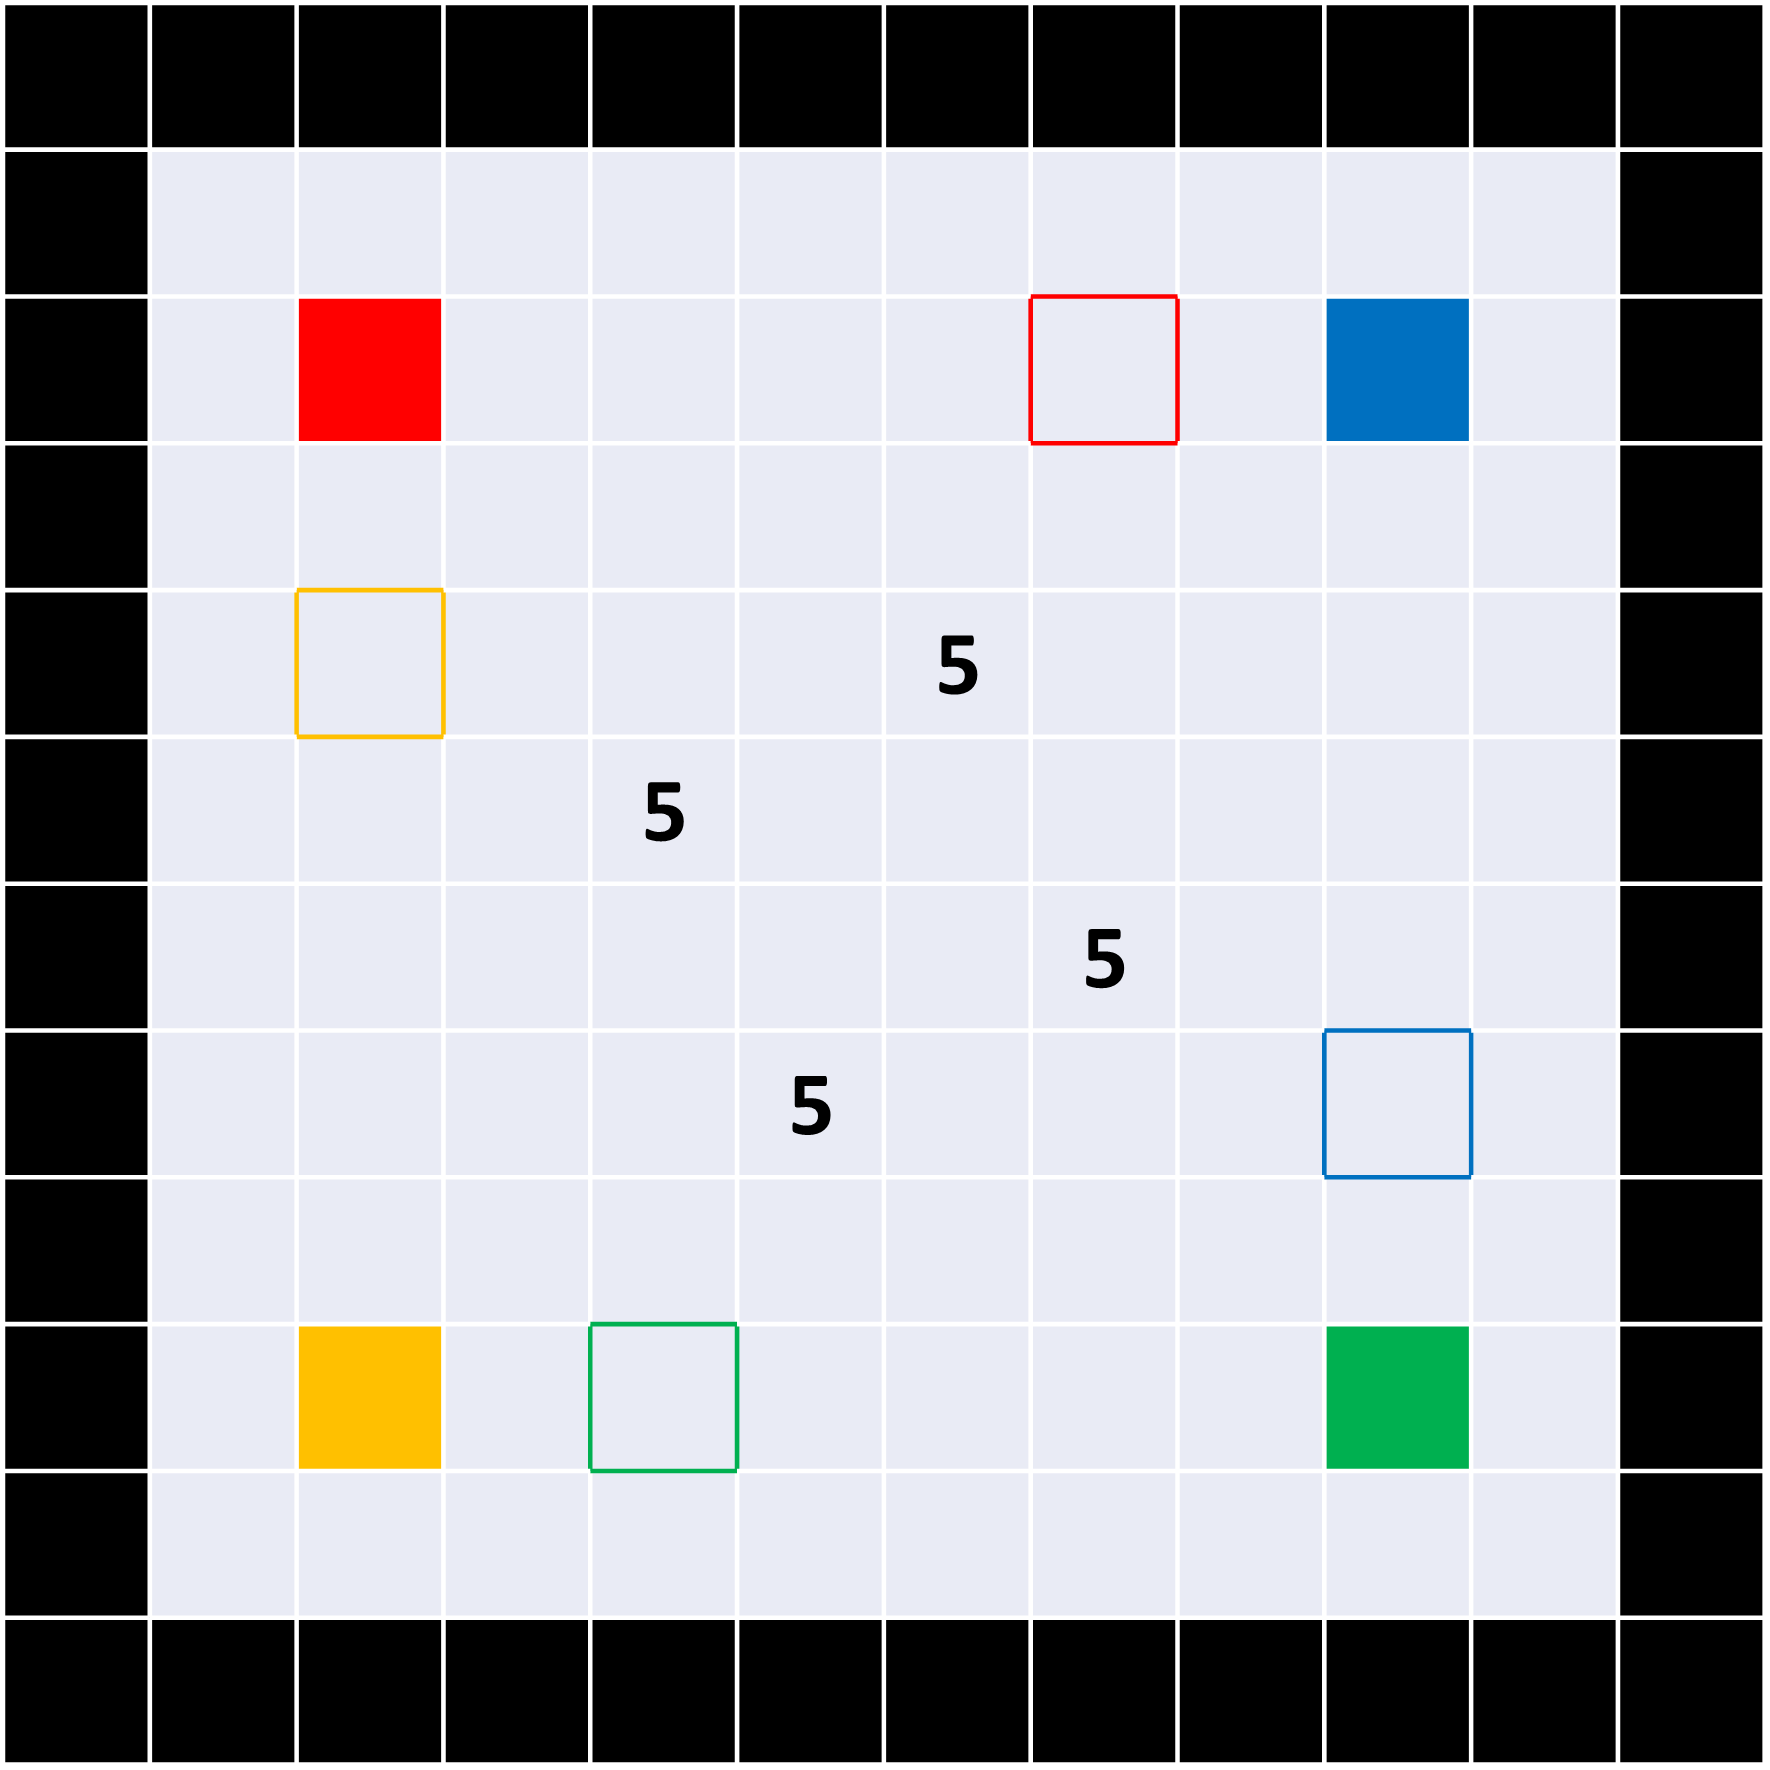
\includegraphics[width=0.1425\textwidth]{Images/P3-4a.png}
%         \label{subfig:l2}}
%     \subfigure[$L_3$]{
%         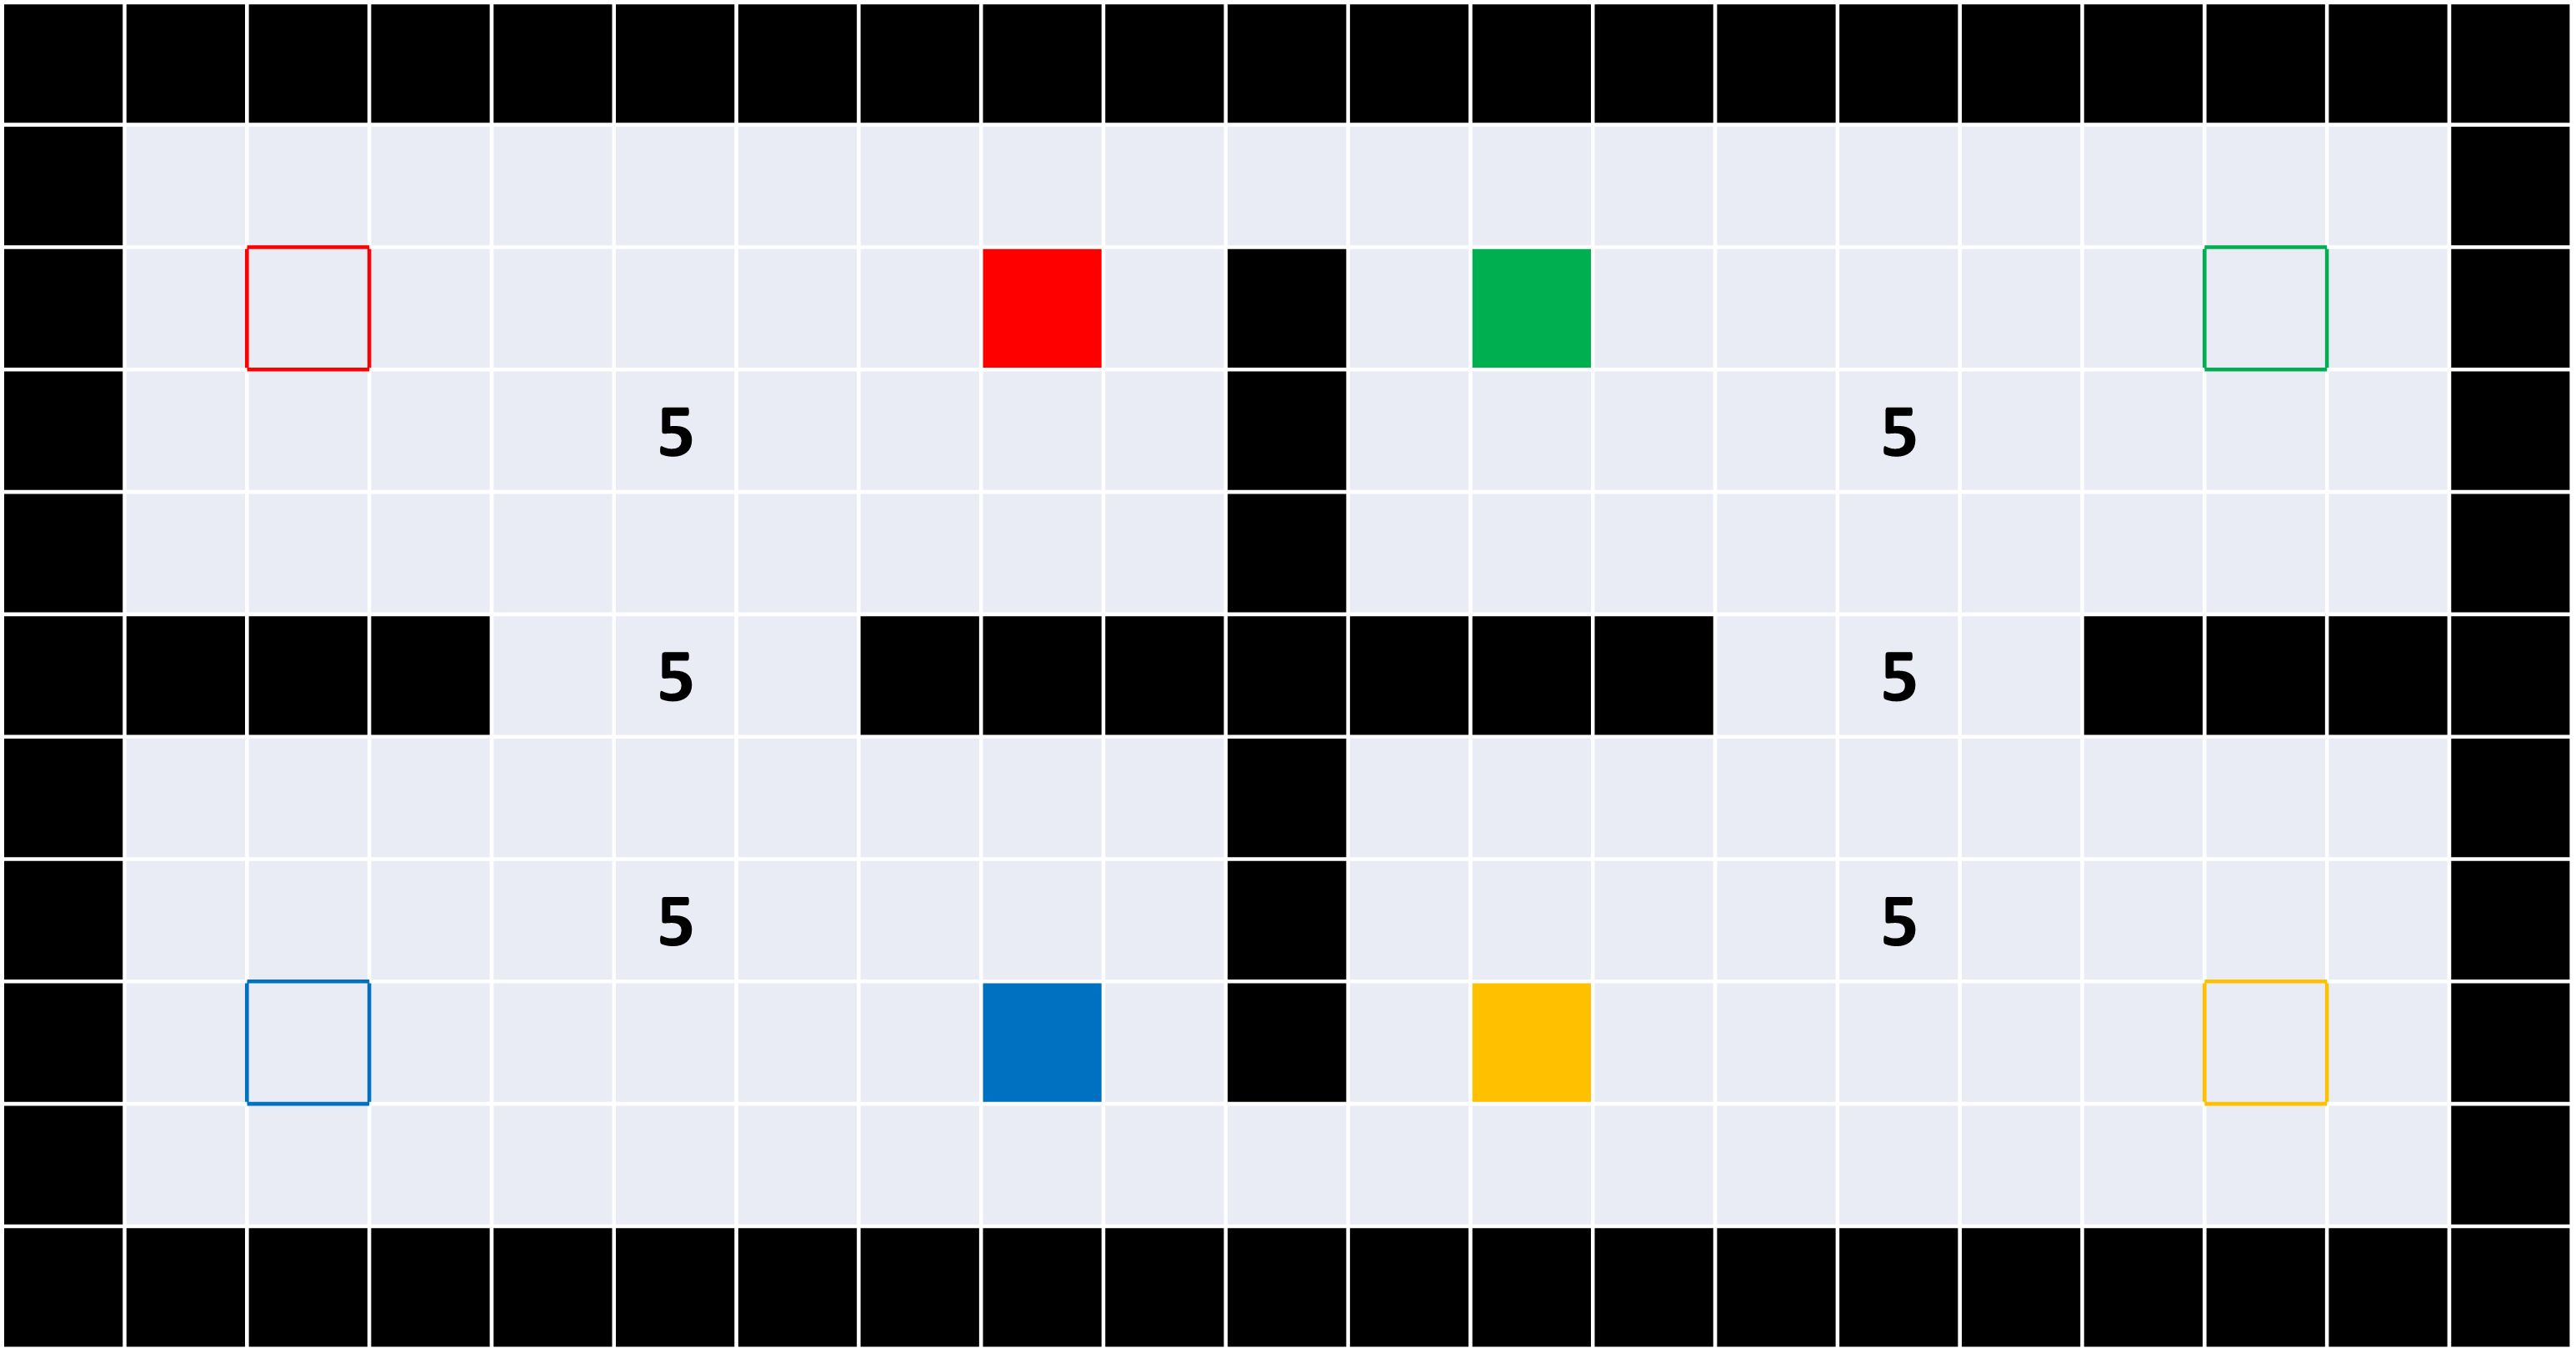
\includegraphics[width=0.27\textwidth]{Images/P2-4a.png}
%         \label{subfig:l3}} 
%     \caption{Grid SMAPF-PO benchmarks. Each color represents an agent. Initial positions are filled. Goal positions are bordered.}
%     \label{fig:multi-problems}
% \end{figure*}


\begin{figure}[t]
\centering
     \subfigure[$S_3$]{
        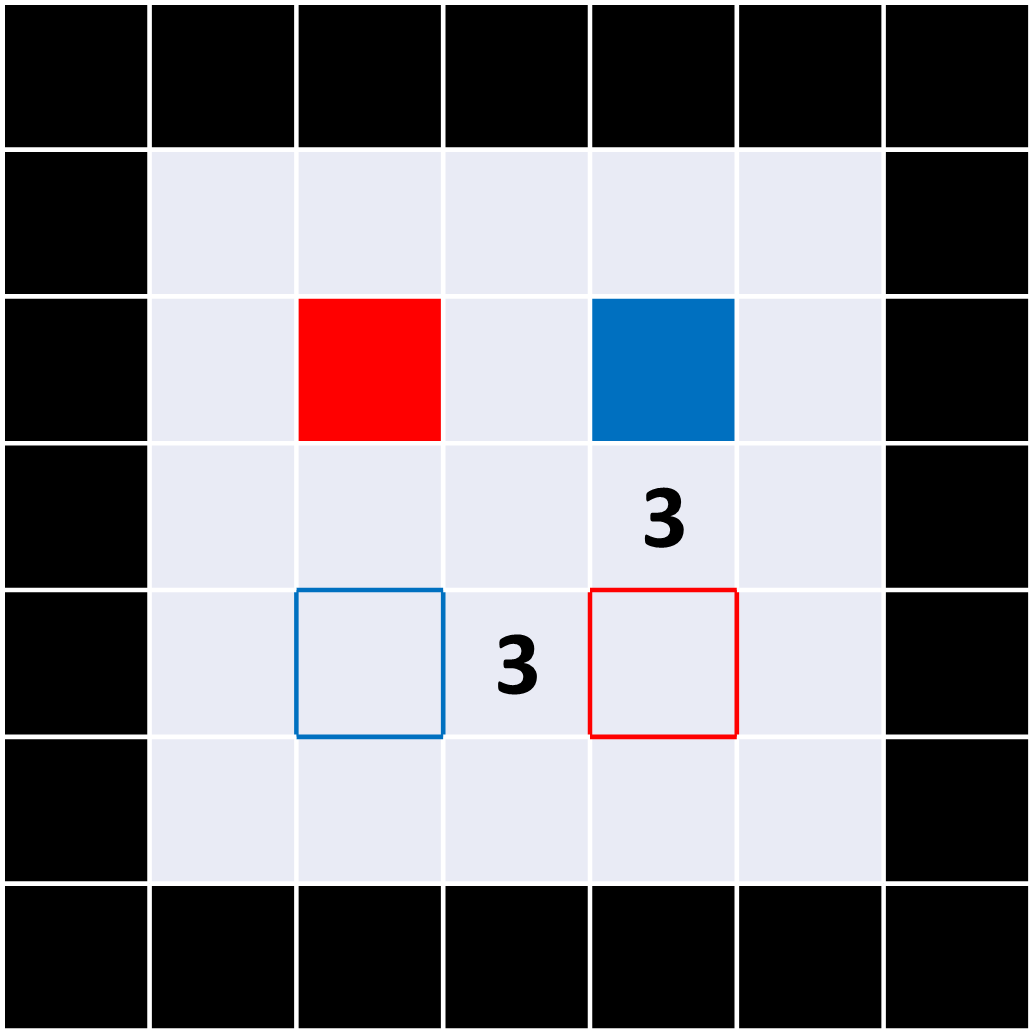
\includegraphics[width=0.15\columnwidth]{Images/P3s.png}
         \label{subfig:s3}}
     \subfigure[$M_3$]{
        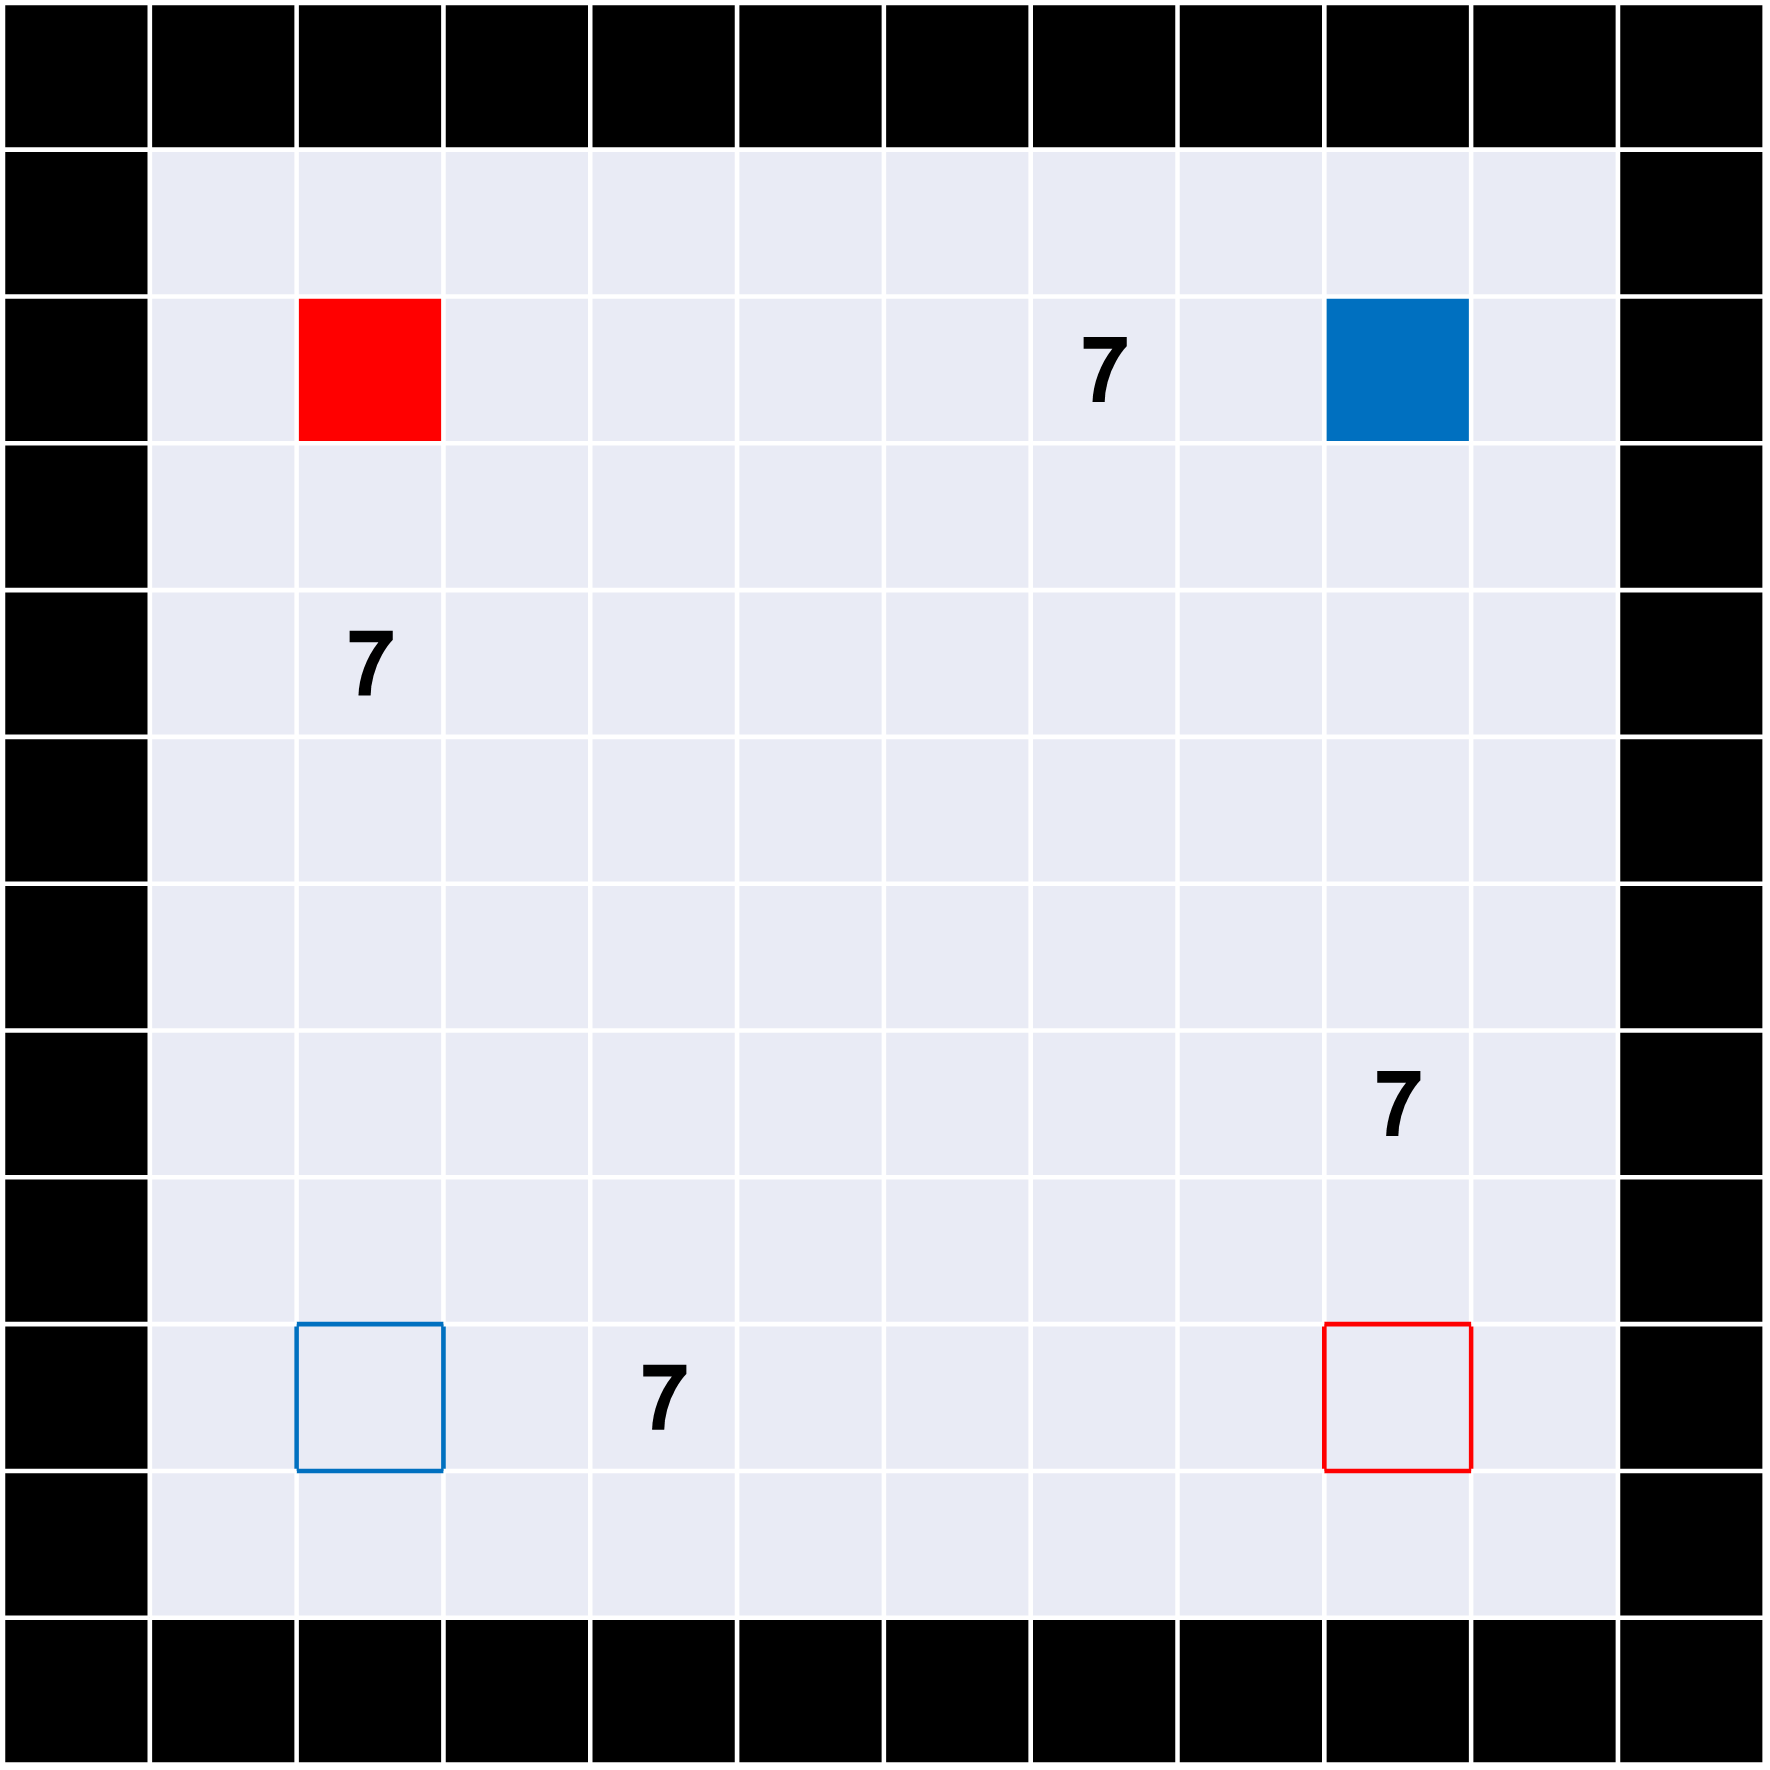
\includegraphics[width=0.25\columnwidth]{Images/P3.png}
         \label{subfig:m3}}
     \subfigure[$L_3$]{
         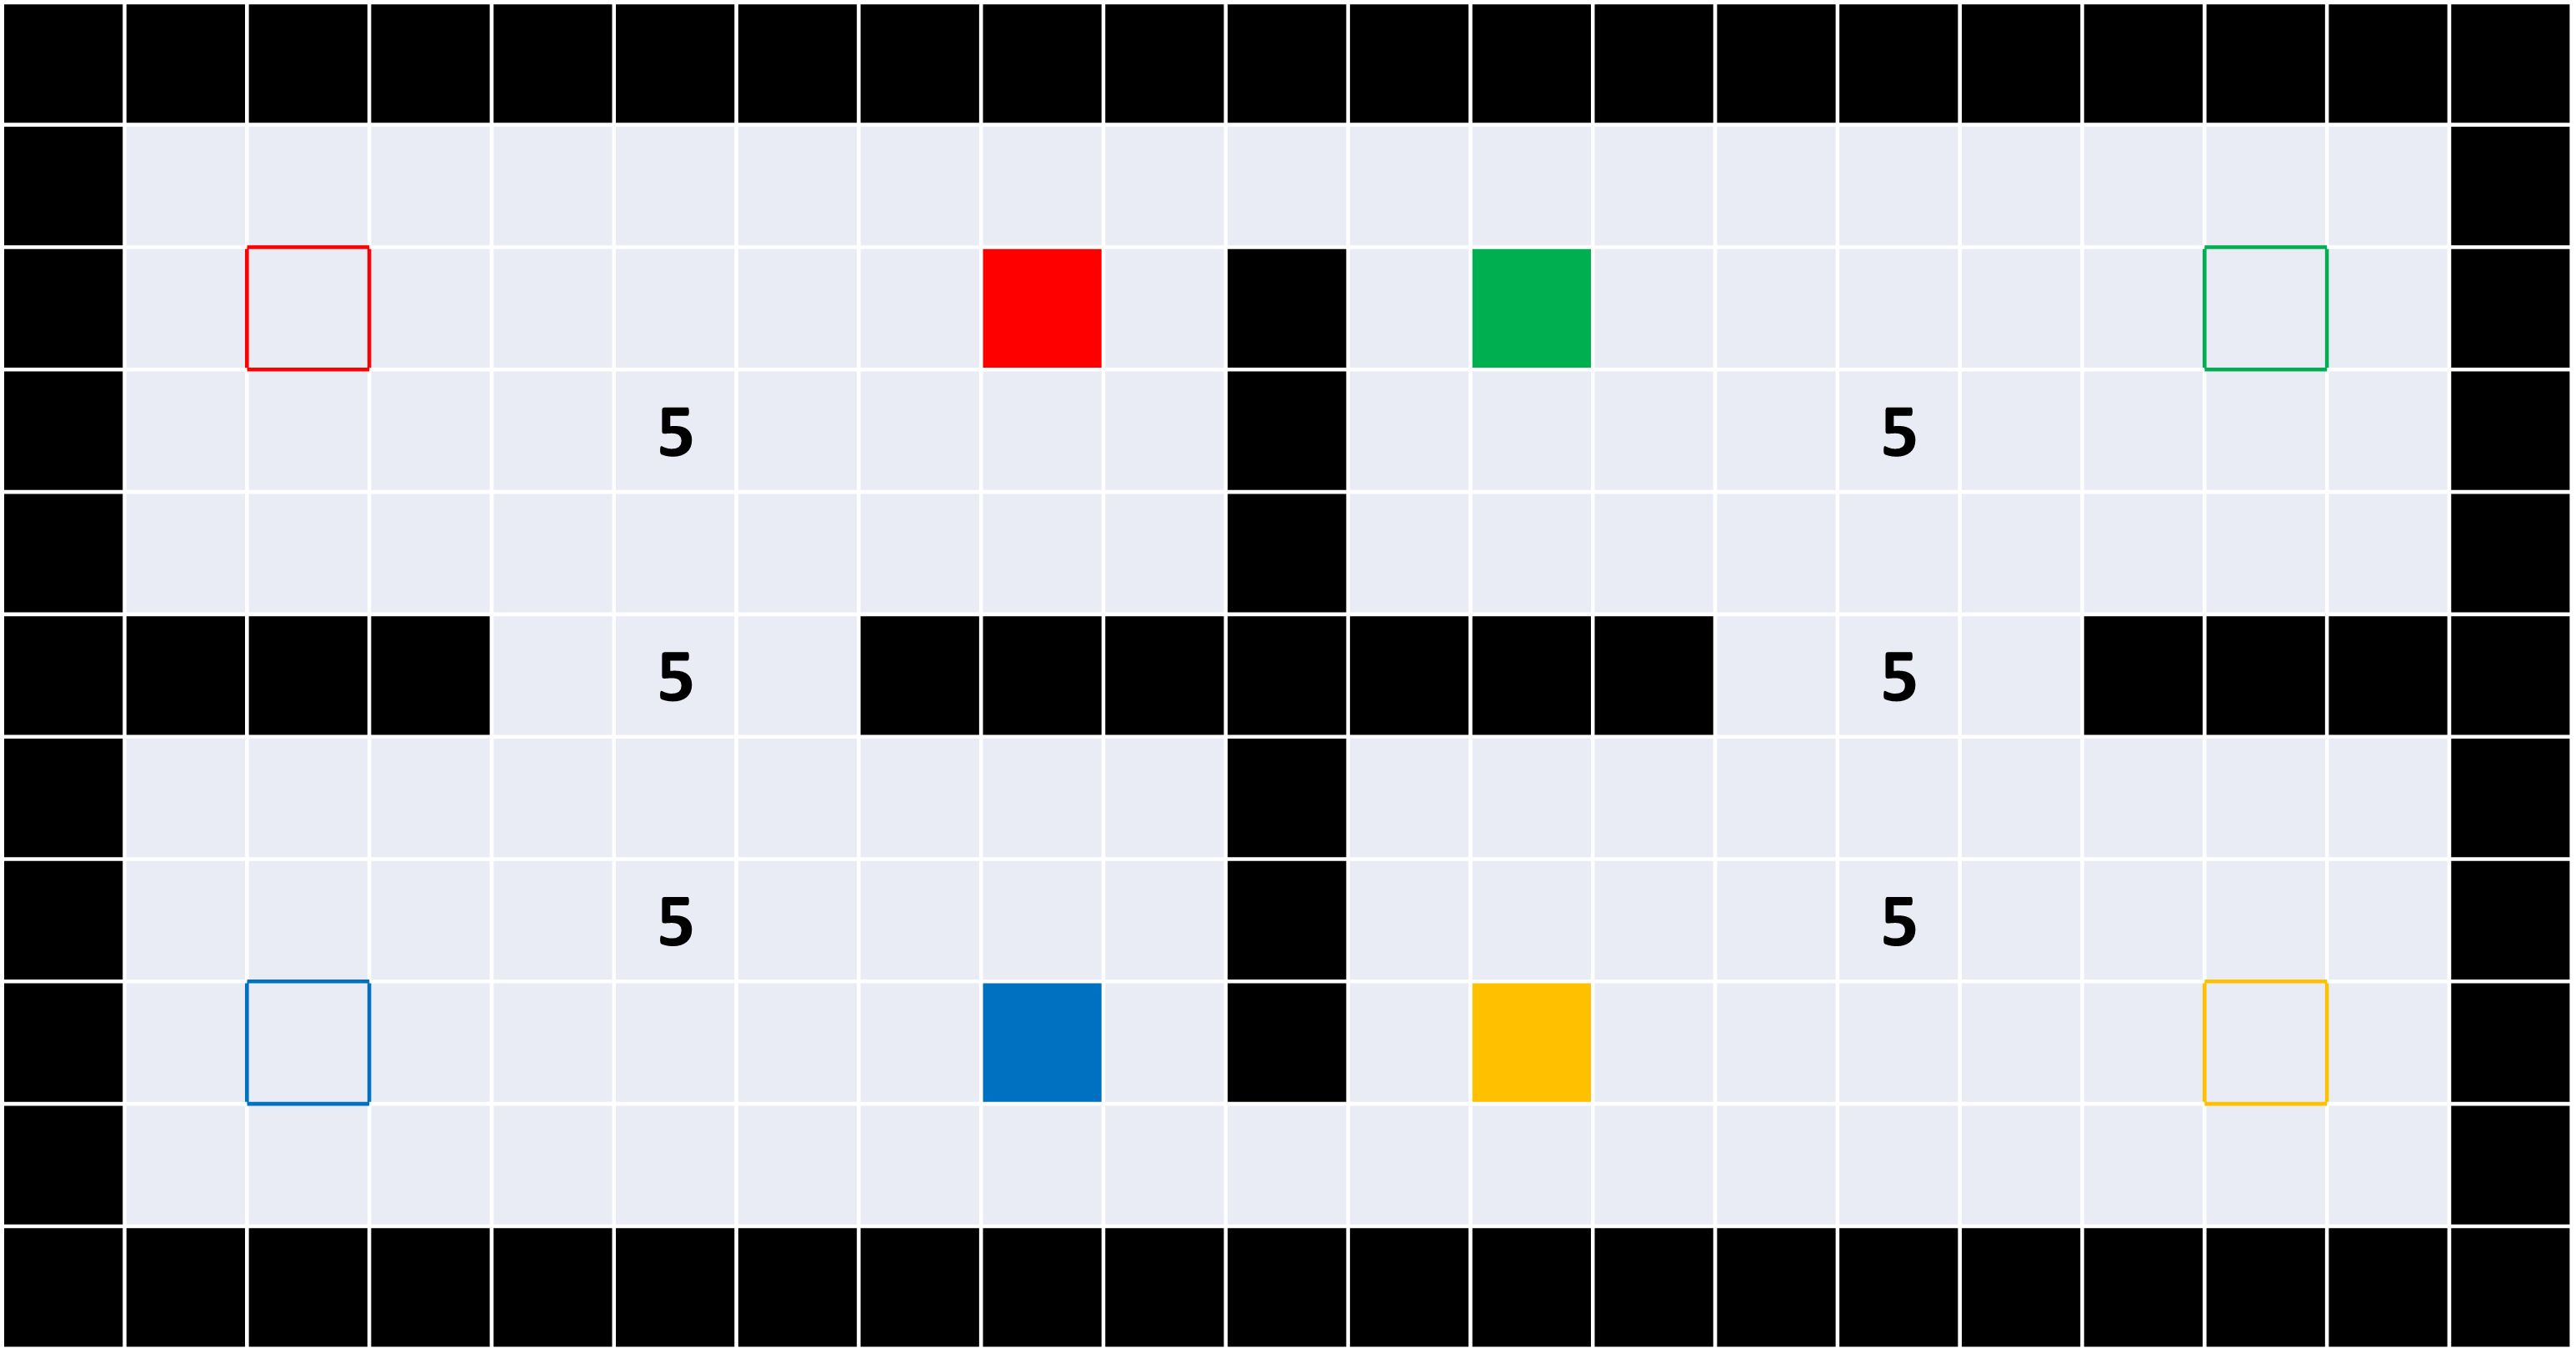
\includegraphics[width=0.45\columnwidth]{Images/P2-4a.png}
         \label{subfig:l3}} 
     \caption{Example grids. Each color represents an agent. Initial cells filled, goal cells bordered.}
     \label{fig:multi-problems}
\end{figure}

% Domains
\noindent\textbf{Benchmarks:}
Solving SMAPF-PO is much more difficult compared to classical MAPF, and none of our algorithms were able to scale to solve SMAPF-PO problems on standard MAPF benchmarks~\cite{stern2019mapf}. 
Instead, we create a suite of 12 SMAPF-PO problems of different sizes, configurations, and number of agents. 
Figure~\ref{fig:multi-problems} illustrates some of these problems visually and Table~\ref{tab:benchmark} provides additional information. 
The supplementary material contains a visualization of all problems in our benchmark. 


Agents' start and goal positions are filled and bordered cells, respectively, where each agent has a different color. Cells with beacons are marked with a number that specifies the beacon's maximal range.  
Our benchmark selection is designed to examine different interactions between the agents and different difficulty levels.
Most of these benchmarks are very difficult given noisy partial observability --- there are no beacons at the goal positions allowing the agent to know it has arrived at the goal. Goal positions are also not located in places that are easy to reach blindly, such as corners. As such, achieving near perfect success is highly unlikely.

As can be seen in Table~\ref{tab:benchmark}, the joint problem rapidly becomes unmanageable, due to the huge joint state space, but also due to the joint action and observation spaces. Each additional beacon adds another action, and the number of observations depends on the range of the beacons.


\noindent\textbf{Baselines:} An experimental comparison between OPP and classical MAPF algorithms is not possible, as the latter assume only one (deterministic) outcome for each action and perfect localization. 
The main contribution of our approach is the decoupling method, that allows use to solve smaller single agent problems, rather than tackle the complete joint problem. We hence compare methods that solve the joint problem to our decoupling approach. For the joint problem, we used both an offline solver, FSVI \cite{shani2013survey}, and an online solver, POMCP \cite{silver2010monte}, with a domain specific heuristic that moves towards the goal. We refer to the joint baselines as \em{Joint-FSVI}, and \em{Joint-POMDP}. %\guy{make sure that we maintain the naming conventions below below}

For our decoupled approach, we also use both FSVI and POMCP to solve the decoupled single agent problems. We denote the OPP POMCP version, which we ran with our forced localization method, as \emph{POMCP+FL}.
We also experiment with several variations of OPP with FSVI: (1) a vanilla method without forcing localizations and without our modified version of FSVI, denoted \emph{FSVI} (2) OPP with the modified FSVI, denoted \emph{FSVI+MF},  (3) OPP with regular FSVI and forced localization, denoted \emph{FSVI+FL}, and (4) OPP with the modified FSVI and forced locatization, denoted \emph{FSVI+MF+FL}. 
%We denote the FSVI variations as \emph{Online}, \emph{FSVI+MF}, and \emph{On.+FL}. The complete version of OPP is denoted by \emph{FSVI+MF+FL}.  
We use FSVI as preliminary experiments with other point-based approaches, namely, Persues and PBVI, did not work as well. That being said, any other offline or online solver can also be used.



%We have compared OPP to the reduction-based approach described above using an offline POMDP solver, namely FSVI~\cite{shani2007forward}. 
%We refer to this baseline as \emph{Offline}. In preliminary experiments we tried  other point-based algorithms\cite{shani2013survey}, such as Perseus and GapMin, but FSVI performed the best. Online POMDP solvers such as POMCP\cite{silver2010monte} usually require 
%strong problem-specific heuristic to work well. It is unclear if heuristics for single agent maze navigation can be easily extended to solve SMAPF-PO problem efficiently. Furthermore, previous attempts to adapt POMCP to multi-agent scenarios were not too successful \cite{badyal2021comparative,zhou2019centralized,chen2015multi}.  
%To better understand the importance of the various components of our method, 

The implementation is in Java. Experiments were run on an AMD\textsc{\textregistered} EPYC 7702P 64-Core with 32 GB of RAM.



\noindent\textbf{Experiment Design and Metrics:}
For every problem in our benchmark we run each of the evaluated algorithms 50 times. 
Every such run was terminated when either all agents have declared that their goal has been reached or when the overall number of steps exceeded 200. In the latter case, we forced all remaining agents to perform a declare action. 


The main performance metric we considered is the average sum of discounted rewards (ADR), which is a common solution quality measure in the POMDP literature. 
We also report the standard error of these averages, the average runtime in seconds, 
and the \emph{success rate}, which is the percentage of runs where all agents reach their respective goal states and performed the declare action appropriately. 
ADR is not directly correlated with the success rate: when one agent reaches the goal and the other does not, declaring done will produce a positive ADR will not be considered a success. This can be seen in our results, where some cases with 0\% success rate still have positive ADR. 
% We can see in the results below several cases where, even given a success rate of $0\%$, a positive ADR is obtained.

 





\paragraph{Results} 

The results for small problems are shown in Table~\ref{tab:2small-results} . 
Columns ``P'', ``RT'', and ``\%S'' specify the problem name, runtime in seconds, and the success rate, respectively. 
% To provide deeper insight into the algorithms' behaviors, 
We also report the number of potential collisions detected and the number of times an agent replanned, denoted as ``\#C'' and ``\#R'', respectively. 
$\#C$ and $\#R$ are always zero for \emph{Offline}, since its initial policy is conflict-free. %its policy 
% As \emph{Offline} generates a policy offline that avoids conflicts, it does not check for potential conflicts and never replans. So, $\#C$ and $\#R$ for Offline are always zero. % and is not reported. 

% As expected, the Joint-FSVI baseline could only solve in reasonable time the smaller 5x5 problems, $S_1$, $S_2$, $S_3$, and $S_4$. On the other hand, the Joint-FSVI managed in some problems to provide the best policy, both with respect to success rate, and with respect to ADR. This is expected, as an optimal POMDP solver on the joint problem, given enough runtime, can return an optimal policy. 
As expected, Joint-FSVI could only solve in reasonable time the smaller 5x5 problems, $S_1$, $S_2$, $S_3$, and $S_4$. On the other hand, Joint-FSVI managed in some problems to provide the best policy in terms of success rate and ADR. This is expected, as an optimal POMDP solver on the joint problem, given enough runtime, can return an optimal policy. Joint-POMCP could not scale beyond  the smallest problem, due to the large number of joint actions and observations.
% branching factor, given the amount of joint actions and observations.



The online algorithms perform well on $S_1$ and $S_2$, where the agents' shortest path to their goals do not conflict. 
However, they perform poorly in $S_3$ and $S_4$, which represent very difficult problems, where agents must move close together in a tight space. As such, the number of conflicts between the shortest paths is very high, many potential conflicts will be detected and the agents will replan very often. This is clearly observable in the ``\#C'' and ``\#R'' results, which are high and are inversely correlated with the ADR.

Another observation from these results is that when many conflicts are expected ($S_3$ and $S_4$), the modified FSVI technique is not beneficial, but the forced localization works better than the vanilla FSVI. 
This is because in such small grids localizing is very helpful, allowing agents to move at least one step without colliding, and then localizing again. 
Looking at the run time of the different algorithms, as expected, computing the joint policy is much more computationally demanding, requiring many orders of magnitude additional run time compared to the online algorithms. Indeed, the offline algorithm could not scale to any of the larger problems. 

The POMCP+FL is slower than all other online methods. This is because even the single agent problems have a relatively large number of actions (movements + pinging beacons), and many observations. Thus, the branching factor is difficult to handle. On the other hand, POMCP+FL creates in some cases good policies, and in $S_2$, even the best policies.





\begin{table}
    \centering
    \resizebox{0.8\columnwidth}{!}{
    \begin{tabular}{ |c|l|c|r|c|c|c| } 
    \hline
    P & Alg & ADR & RT & \% S & \#C & \#R \\
    % \hline\hline
    % \multicolumn{7}{|c|}{\ref{subfig:s1}} \\
    \hline
    \multirow{7}{*}{$S_1$}  
    & Joint-FSVI\itay{+} & 80 $\pm$ 4 & 671 & 85\% & - & - \\ 
    & Joint-POMCP\itay{+} & 56$\pm$6 & 78\itay{**} & 48\% & - & -\\
    %\hline
    & POMCP+FL\itay{+} & 55 $\pm$ 6 & 3 & 68\% & 0.04$\pm$0.03 & 0.04$\pm$0.03 \\ 
     & FSVI\itay{+} & 80 $\pm$ 4 & 3 & 88\% & 0.5$\pm$0.1 & 0.5$\pm$0.2 \\
   & FSVI+MF\itay{+} & 76 $\pm$ 4 & 2 & 80\% & 0.3$\pm$0.1 & 0.4$\pm$0.1 \\
    %\hline
    &FSVI+FL\itay{+} & \textbf{79 $\pm$ 4} & 3 & 88\% & 0.5$\pm$0.1 & 0.5$\pm$0.2\\ 
    %\hline
    & FSVI+MF+FL\itay{+} & 74 $\pm$ 5 & 5 & 76\% & 2$\pm$2 & 4$\pm$4 \\
    % \hline
    % \hline
    % \multicolumn{7}{|c|}{\ref{subfig:s2}} \\
    \hline
    \hline
    \multirow{5}{*}{$S_2$}  
    & Joint-FSVI\itay{+} & 62 $\pm$ 6 & 692 & 72\% & - & - \\
    & Joint-POMCP &&&&& \\
    & POMCP+FL\itay{new} & 63 $\pm$ 4 & 106 & 68\% & 130$\pm$28 & 131$\pm$28 \\
     & FSVI\itay{+} & 61 $\pm$ 5 & 11 & 64\% & 5$\pm$0.8 & 7$\pm$1 \\
   & FSVI+MF\itay{+} & 49 $\pm$ 5 & 23 & 40\% & 6$\pm$3 & 10$\pm$4 \\
    &FSVI+FL\itay{+} & 64 $\pm$ 6 & 41 & 80\% & 27$\pm$5 & 10$\pm$11 \\
    & FSVI+MF+FL\itay{+} & 48 $\pm$ 7 & 50 & 62\% & 41$\pm$6 & 80$\pm$13 \\ 
    % \hline
    % \hline
    % \multicolumn{7}{|c|}{\ref{subfig:s3}} \\
    \hline
    \hline
    \multirow{5}{*}{$S_3$} 
    & Joint-FSVI\itay{+} & 3 $\pm$ 4 & 3516 & 10\%  & - & - \\ 
    & Joint-POMCP &&&&& \\
    & POMCP+FL\itay{+} & 0 $\pm$ 4 & 331 & 12\% & 90$\pm$6 & 170$\pm$10 \\
    & FSVI\itay{+} & 21 $\pm$ 1 & 17 & 0\% & 2.7$\pm$0.1 & 4.3$\pm$0.2 \\
    & FSVI+MF\itay{+} & 17 $\pm$ 3 & 21 & 0\% & 2.4$\pm$0.1 & 3.9$\pm$0.2 \\
    &FSVI+FL\itay{+} & 11 $\pm$ 5 & 68 & 18\% & 66$\pm$7 & 128$\pm$13 \\
    & FSVI+MF+FL\itay{+} & 3 $\pm$ 4 & 93 & 10\% & 70$\pm$6 & 138$\pm$13 \\
    % \hline
    % \hline
    % \multicolumn{7}{|c|}{\ref{subfig:$S_4$}} \\
    \hline
    \hline
    \multirow{5}{*}{$S_4$} 
    & Joint-FSVI\itay{+} & 57 $\pm$ 6 & 4735 & 63\% &  - & - \\ 
    & Joint-POMCP &&&&& \\
    & FSVI\itay{+} & 22 $\pm$ 1 & 9 & 0\% & 2$\pm$0 & 3$\pm$0 \\
    & POMCP+FL\itay{+} & -12.2 $\pm$ 0 & 422 & 0\% & 99.7$\pm$0.06 & 199$\pm$0.1 \\
    & FSVI+MF\itay{+} & 22 $\pm$ 0.6 & 5 & 0\% &  2$\pm$0 & 3$\pm$0 \\
    &FSVI+FL\itay{+} & 21 $\pm$ 5 & 57 & 36\% & 58$\pm$6 & 112$\pm$13 \\
    & FSVI+MF+FL\itay{+} & -12 $\pm$ 0 & 203 & 0\% &  100$\pm$0 & 200$\pm$0 \\
    \hline
    \hline
     \end{tabular}
     }
    \caption{Results for small problems ($S_1$, $S_2$, $S_3$, and $S_4$).\itay{** Average run-time in 200 runs}}
    \label{tab:2small-results}
    \vspace{-0.3cm}
\end{table}




\noindent\textbf{Results on large problems}
Table~\ref{tab:large-results} lists the results for the larger problems ($M_1$, $M_2$, $M_3$, $M_4$, $M_5$, $L_1$, $L_2$, and $L_3$), where the joint problem is too difficult for FSVI and POMCP. 
In these problems, the benefit of the forced localization (FL) method are obvious. 
For example, without FL and MF the success rate of the vanilla FSVI was 0 for $M_3$, $M_4$, $M_5$, and $L_2$, while 
FSVI+FL and FSVI+MF+FL often succeed. This advantage is also shown in the ADR. 
For example, in $L_1$ using FL approximately doubled the ADR achieved. 


The benefit of modifying FSVI (MF) to include more pings, however, is less pronounced. Only in $M_1$ FSVI+MF provides better results than FSVI+FLm while in most cases, using only FSVI+MF in not as good as FSVI+FL. On the other hand, the combined FSVI+FL+MF provides additional leverage, at least in the largest problem, $L_3$.

POMCP-FL provided competetive results in some cases, but in most problems did not work as well as FSVI-FL. On the largest problems, POMCP-FL failed to provide strong policies, probably because the longer needed planning horizon requires deeper trees, which take a long time to construct.

In some sense, $M_5$ is the hardest of the large problems, as the single-agent path of each agent to its goal is conflicting in $M_5$, requiring much coordination for navigating the narrow corridors without collisions. 
Additional research is needed to develop methods that can better handle such problems that require strong synchronization. It may be that in such corridors, solving a small, short range joint problem is better.

\noindent\textbf{Summary} For very small problems, finding a solution to the joint problem provides the best policy, but takes a very long time. As such, only OPP was able to scale beyond very small problems, especially when using the FL method. This demonstrates that solving the naive joint MAPF POMDP problem is not practical, and hence, one would need to use some type of decoupling technique, creating single agent problems that allow for much better scaling up.

We also see here that domain specific techniques can help POMDP solvers in creating better policies, with respect to the synchronization of policies. Our localization additions were successful because, when considering a single agent, localization is less important, unless we are near the goal. However, when other agents are nearby, localization can reduce significantly the possibility for collisions, and hence, the need to replan, and the constraints during replanning.




\section{Related Work}

MAPF with unexpected delays has been studied in different forms~\cite{atzmon2020probabilistic,shahar2021safe,atzmon2020robust,ma2017multiAgent}. Yet limiting stochastic effects to delays simplifies the problem compared to SMAPF-PO, and these works all assumed perfect observability. 
$UM^*$~\cite{wagner2017path} does support uncertainty over agents' locations but it allows agents to risk conflicts as long as their probability of occurring is beneath a given threshold. Similarly, prior work on multi-robot navigation assigned cost to collision and aim to minimize it. 
%$UM^*$~\cite{wagner2017path} is a complete MAPF algorithm designed for stochastic delays and uncertainty over agents' locations. However, it allows agents to risk conflicts as long as their probability of occurring is beneath a given threshold. Similarly, prior work on multi-robot navigation assigned cost to collision and aim to minimize it. 
The SMAPF-PO is fundamentally different since we require avoiding any chance for having a conflict. % at all cost. 
Recent work~\cite{davydov2021q} on MAPF with partial observability differs from SMAPF-PO in that they assumed control is not centralized and agents' visibility is based on line of sight. The latter assumption is different from our beacons-based observation model, precluding empirical comparison.


% Relation to MMDP
MAPF under movement uncertainty is a special case of Multi-Agent MDP (MMDP)~\cite{boutilier1996planning}. 
General-purpose MMDP solvers~\cite{de2021constrained} do not exploit the specific structure of the SMAPF-PO problem, such as the limited interactions between agents. Similarly, online approaches for solving large MDPs, such as FF-Replan\cite{yoon2007ff}, are not expected to be effective in our domain and do not deal with partial observability. 
% Relation to POMDP and DecPOMDP
Dec-POMDP~\cite{oliehoek2012decentralized} is often used to model multi-agent problems under partial observability, where agents plan jointly, but execute their policies independently.
This is different from our setting, where agents are controlled in a centralized manner and share their observations. 
Also, Dec-POMDP algorithms tend to scale poorly unless the interactions between the agents are limited to small predefined areas in the state space~\cite{melo2009learning}. 
Multiagent POMDP~\cite{oliehoek2017madp}, where both planning and control are centralized, is an appropriate model for SMAPF-PO.  \citet{amato2015scalable} suggest an algorithm based on POMCP which exploits the locality of agent interactions. 
% They construct search trees for disjoint sets of highly coupled agents independently. 
Their algorithm given singleton sets is similar to our POMCP, which does not scale as well as FSVI. 
% Our approach overcomes the necessity to consider several agents jointly by using PP, and hence can scale better. 
Our approach can be viewed as a particular implementation of FT-POMCP leveraging the structure of the SMAPF-PO problem for factorization, and using prioritized planning to ensure independence.

Factorizing the decision-making process in POMDPs has long roots \cite[e.g.]{shani2008efficient,veiga2014point}, and is particularly useful given several independent tasks. 
% , a factored representation can be highly useful. 
Factorization is less effective, however, when the coupling between the tasks increases, as happens in our problem where agents may collide. In tasks with high uncertainty concerning the current state, such coupling is common, and useful factoring is difficult. 
We used FSVI and POMCP but other alternatives for offline and online POMDP solvers exist \cite[e.g.]{walraven2019point,kurniawati2016online,ye2017despot}. Our contribution  is not in an adaptation of a particular POMDP solver to SMAPF-PO, but in our factoring and prioritization schemes. Replacing POMCP with, e.g., ABT, is likely to scale up only slightly, while improvements to the factorization can make a huge difference.


% MAPF with unexpected delays have been studied in different forms~\cite{atzmon2020probabilistic,shahar2021safe,atzmon2020robust,ma2017multiAgent}. Yet limiting stochastic effects to delays simplifies the problem compared to SMAPF-PO, and these works all assumed perfect observability. 
% $UM^*$~\cite{wagner2017path} is a complete MAPF algorithm designed for stochastic delays and uncertainty over agents' locations. However, it allows agents to risk conflicts as long as their probability of occurring is beneath a given threshold. 
% Similarly, prior work on multi-robot navigation assign cost to collision and aim to minimize it. 
% These works are fundamentally different from our problem since we require avoiding any chance for having a conflict at all cost. 
% Recent work~\cite{davydov2021q} on MAPF with partial observability differs from SMAPF-PO in that they assumed control is not centralized and agents' visibility is based on line of sight. The latter assumption is different from our beacons-based observation model, which precludes experimental comparison with their algorithm. 
% applied a Multi-Agent Reinforcement Learning (MARL) technique, specifically the QMIX algorithm~\cite{rashid2018qmix}. MARL techniques do not exploit knowledge the world's model. In addition, their MAPF setting was fundamentally different --- control was not centralized and agents visibility was based on line of sight. 

% $UM^*$~\cite{wagner2017path} is designed for stochastic effects in the forms of unexpected delays, and uncertainty over agents' locations. 
% They allow agents to risk conflicts as long as their probability of occurring is beneath a given threshold, which is fundamentally different from our requirement to avoid all conflicts. 
% Similarly, 
% Prior work on multi-robot navigation assign cost to collision and aim to minimize it. 
% Similarly, $UM^*$~\cite{wagner2017path}, which is designed for MAPF stochastic delays and allows and uncertainty over agents' locations, allows agents to risk conflicts as long as their probability of occurring is beneath a given threshold. 
% These works are fundamentally different from our problem since we require avoiding any chance for having a conflict at all cost. 





\begin{table}
    \centering
    \resizebox{0.8\columnwidth}{!}{
    \begin{tabular}{ |c|l|c|r|c|c|c| } 
    \hline
    P & Alg & ADR & RT & \% S & \#C & \#R \\
    % \hline\hline
    % \multicolumn{7}{|c|}{\ref{subfig:s1}} \\
    \hline
    % \multicolumn{7}{|c|}{\ref{subfig:m1}} \\
    \hline
    \multirow{4}{*}{$M_1$}      
    & FSVI\itay{+} & 69 $\pm$ 4 & 21 & 74\% & 0.3$\pm$0.1 & 0.4$\pm$0.2 \\
    & POMCP+FL\itay{+} & 52 $\pm$ 5 & 33 & 62\% & 15$\pm$12 & 16$\pm$13 \\
    & FSVI+MF\itay{+} & 70 $\pm$ 4 & 19 & 78\% & 0.4$\pm$0.2 & 0.6$\pm$0.2 \\
    &FSVI+FL\itay{+} & 61 $\pm$ 5 & 22 & 66\% & 0.2$\pm$0.1 & 0.3$\pm$0.2 \\ 
    & FSVI+MF+FL\itay{+} & 70 $\pm$ 4 & 18 & 78\% &  0.4$\pm$0.2 & 0.6$\pm$0.2 \\
    \hline
    % \multicolumn{7}{|c|}{\ref{subfig:m2}} \\
    \hline
    \multirow{4}{*}{$M_2$}      
    & FSVI\itay{+} & 41 $\pm$ 5 & 146 & 46\% & 4$\pm$0.4 & 7$\pm$0.6 \\
    & POMCP+FL\itay{+} & 28 $\pm$ 5 & 946 & 46\% & 300$\pm$20 & 300$\pm$20 \\
    & FSVI+MF\itay{+} & 28 $\pm$ 4 & 230 & 30\% & 5$\pm$0.3 & 7$\pm$0.4 \\
    &FSVI+FL\itay{+} & 48 $\pm$ 5 & 191 & 64\% & 6$\pm$0.5 & 9$\pm$0.6 \\
    & FSVI+MF+FL\itay{+} & 55 $\pm$ 4 & 200 & 76\% & 5$\pm$0.4 & 8$\pm$0.5 \\ 
    \hline\hline
    % \multicolumn{7}{|c|}{\ref{subfig:m3}} \\
    % \hline
    \multirow{4}{*}{$M_3$}      
    & FSVI\itay{+} & 17.8 $\pm$ 0.4 & 253 & 0\% & 1$\pm$0 & 2$\pm$0 \\
    & POMCP+FL\itay{+} & 57 $\pm$ 3 & 202 & 84\% & 79$\pm$15 & 83$\pm$15 \\
    & FSVI+MF\itay{+} & 17.6 $\pm$ 0.3 & 418 & 0\% & 1$\pm$0 & 2$\pm$0 \\
    &FSVI+FL\itay{+} & 56 $\pm$ 3 & 402 & 92\% & 10$\pm$1 & 16$\pm$3 \\
    & FSVI+MF+FL\itay{+} & 48 $\pm$ 4 & 535 & 72\% & 10$\pm$2 & 18$\pm$3 \\
    \hline\hline
    % \multicolumn{7}{|c|}{\ref{subfig:m4}} \\
    % \hline
    \multirow{4}{*}{$M_4$}      
    & FSVI\itay{+} & 30 $\pm$ 3 & 133 & 10\% & 1$\pm$0 & 2$\pm$0 \\
    & POMCP+FL\itay{+} & 73 $\pm$ 2 & 208 & 94\% & 63$\pm$16 & 63$\pm$16 \\
    & FSVI+MF\itay{+} & 36 $\pm$ 4 & 91 & 20\% & 1$\pm$0 & 2$\pm$0 \\
    &FSVI+FL\itay{+} & 77 $\pm$ 7 & 245 & 96 \% & 2$\pm$0.3 & 4$\pm$0.4 \\
    & FSVI+MF+FL\itay{+} & 75 $\pm$ 3 & 125 & 94\% & 3$\pm$0.7 & 5$\pm$1 \\
    \hline\hline
    % \multicolumn{7}{|c|}{\ref{subfig:m5}} \\
    % \hline
    \multirow{4}{*}{$M_5$}      
    & FSVI\itay{+} & -6 $\pm$ 3 & 381 & 0\% & 2.1$\pm$0.2 & 3.4$\pm$0.2 \\
    & POMCP+FL\itay{+} & -11.6 $\pm$ 0.6 & 275 & 2\% & 55$\pm$5 & 101$\pm$3 \\
    & FSVI+MF\itay{+} & 5 $\pm$ 2 & 217 & 0\% & 2.0$\pm$0.1 & 3.3$\pm$0.2 \\
    &FSVI+FL\itay{+} & -6 $\pm$ 2 & 896 & 8\% & 29$\pm$3 & 55$\pm$6 \\
    & FSVI+MF+FL\itay{+} & 0 $\pm$ 2 & 671 & 2\% & 20$\pm$3 & 37$\pm$5 \\
    \hline\hline
    % \multicolumn{7}{|c|}{\ref{subfig:l1}} \\
    \multirow{4}{*}{$L_1$}
    & FSVI\itay{+} & 37 $\pm$ 6 & 254 & 8\% &  7.2$\pm$0.5 & 10.9$\pm$0.8 \\
    & POMCP+FL\itay{+} & 64 $\pm$ 5 & 1954 & 64\% &  372$\pm$21 & 376$\pm$21 \\
    & FSVI+MF\itay{+} & 29 $\pm$ 6 & 433 & 6\% &  6.8$\pm$0.5 & 10.5$\pm$0.6 \\
    &FSVI+FL\itay{+} & 97 $\pm$ 3 & 222 & 78\% &  8$\pm$0.5 & 12$\pm$0.7 \\ 
    & FSVI+MF+FL\itay{+} & 97 $\pm$ 4 & 386 & 74\% &  10$\pm$3 & 15$\pm$4 \\
    \hline\hline
    % \multicolumn{7}{|c|}{\ref{subfig:l2}} \\
    \multirow{4}{*}{$L_2$}
    & FSVI\itay{+} & -11 $\pm$ 2 & 80 & 0\% &  2.96$\pm$0.02 & 8.8$\pm$0.1 \\
    & POMCP+FL\itay{-} & 69 $\pm$ 12 & 1950 & 26\% &  - & - \\
    & FSVI+MF\itay{+} & -15.1 $\pm$ 0.3 & 57 & 0\% &  3$\pm$0 & 8.9$\pm$0.1 \\
    &FSVI+FL\itay{+} & 67 $\pm$ 12 & 182 & 36\% &  25$\pm$3 & 50$\pm$6 \\
    & FSVI+MF+FL\itay{+} & 73 $\pm$ 11 & 212 & 30\% & 20$\pm$3 & 40$\pm$6 \\
    \hline \hline
    % \multicolumn{7}{|c|}{\ref{subfig:l3}} \\
    % \hline
    \multirow{4}{*}{$L_3$}
    & FSVI\itay{+} & 67 $\pm$ 6 & 202 & 8\% & 8$\pm$0.6 & 12$\pm$0.8 \\
    & POMCP+FL\itay{+} & 35 $\pm$ 7 & 1663 & 12\% & 328$\pm$23 & 326$\pm$22 \\
    & FSVI+MF\itay{+} & 59 $\pm$ 7 & 353 & 8\% & 9$\pm$1 & 13$\pm$1 \\
    &FSVI+FL\itay{+} & 112 $\pm$ 5 & 183 & 62\% & 10$\pm$1 & 14$\pm$1 \\
    & FSVI+MF+FL\itay{+} & 117 $\pm$ 6 & 423 & 68\% & 12$\pm$1 & 18$\pm$2 \\ 
    \hline
    \end{tabular}
    }
    \caption{Results for medium and large problems.}% ($M_1$, $M_2$, $M_3$, $M_4$, $M_5$, $L_1$, $L_2$, and $L_3$).}
    \vspace{-0.3cm}
    \label{tab:large-results}
\end{table}





 
\section{Conclusion}

We studied the Stochastic MAPF with Partial Observability (SMAPF-PO) problem, which is a generalization of MAPF in which actions have stochastic outcomes and agents do not have perfect observability of the current state. We focused on a centralized control setup. While SMAPF-PO can be modeled as a single-agent POMDP problem, solving this POMDP is intractable even for small problems.
We introduced the OPP approach, an online adaptation of Prioritized Planning. OPP has several non-trivial components which we describe, and we also propose two extensions that encourage the agents to actively localize. The results showed that OPP solves larger problems than an offline baseline. 
Yet, solving larger problems is still an open challenge for future work. 





%\ack We would like to thank the referees for their comments, which helped improve this paper considerably

\bibliography{ecai}
\end{document}
%%%%%%%%%%%%%%%%%%%%%%%%%%%%%%%%%%%%%%%%%%%%%%%%%%%%%%%%%%%%%%%%%%%%%%
